% https://github.com/uio-latex/phduio-article-based
% localdefs

\newcommand{\ctext}[3][RGB]{%
  \begingroup
  \definecolor{hlcolor}{#1}{#2}\sethlcolor{hlcolor}%
  \hl{#3}%
  \endgroup
}


%end local defs

% Add [final] to remove marginal notes,
% remove [colophon] for a blank colophon page:
\documentclass[colophon, english]{phduio}

\usepackage{phdstyle}   % Custom style
\usepackage{kantlipsum} % Dummy text


%\makeglossaries
%\newacronym{AMQ}{AMQ}{Approximate Memmbership Query}
%\newacronym{API}{API}{Application Programming Interface}
%\newacronym{BQF}{BQF}{Backpack Quotient Filter}
%\newacronym{cAMQ}{cAMQ}{counting Approximate Memmbership Query}
%\newacronym{CBF}{CBF}{Counting Bloom Filter}
%\newacronym{cli}{cli}{Command Line Interface}
%\newacronym{CNV}{CNV}{Copy Number Variant}
%\newacronym{CQF}{CQF}{Counting Quotient Filter}
%\newacronym{DNA}{DNA}{Deoxyribonucleic acid }
%\newacronym{ENA}{ENA}{European Nucleotide Archive}
%\newacronym{GWAS}{GWAS}{Genome Wide Association Study}
%\newacronym{HiFi}{HiFi}{High Fidelity}
%\newacronym{HPRC}{HPRC}{Human Pangenome Reference Consortium}
%\newacronym{kff}{kff}{\kmer file format}
%\newacronym{MPHF}{MPHF}{Minimal Perfect Hash Functions}
%\newacronym{MSA}{MSA}{Multiple Sequence Alignment}
%\newacronym{NGS}{NGS}{Next Generation Sequencing}
%\newacronym{PCR}{PCR}{Polymerase Chain Reaction}
%\newacronym{QC}{QC}{Quality Control}
%\newacronym{QF}{QF}{Quotient Filter}
%\newacronym{RNA}{RNA}{Ribonucleic acid}
%\newacronym{RSQF}{RSQF}{Rank Select Quotient Filter}
%\newacronym{SIMD}{SIMD}{Single Instruction Multiple Data}
%\newacronym{SNP}{SNP}}{Single Nucleotide Polymorphism}
%\newacronym{SNV}{SNV}}{Single Nucleotide Variant}
%\newacronym{SRA}{SRA}{Sequence Read Archive}
%\newacronym{SV}{SV}{Structural Variation}
%\newacronym{TGS}{TGS}{Third Generation Sequencing}
%\newacronym{T2T}{T2T}{Telomere to Telomere consortium}

%HbS,DARC,STARR-seq, ATAC-seq, ChIP-seq, RNA-seq


\author{Francesco Andreace}
\title{Can I decide it or should I put the official one?}
\subtitle{Analysis of human pangenome graphs using k-mer-based applications}
\department{Department of Computational Biology}
\faculty{Insitut Pasteur Paris, Universite' de Paris Cite}
\affiliation
{
    Edite doctoral school, Sorbonne Université
}
\ISSN{1234-5678}           
\dissertationseries{1234}  


\includeonly
{
    sections/dedication,
    sections/preface,
    sections/abstract-en,
    sections/abstract-fr,
    sections/papers,
    sections/introduction,
    sections/background,
    %sections/cqf,
    %sections/paperI,
    %sections/paperII,
    %sections/paperIII,
    %sections/appendixA,
    %sections/appendixB,
    sections/perspectives,
    sections/pushing_the_limit,
    sections/reducing_complexity,
    sections/explorations
    sections/conclusions,
}


\begin{document}

    \frontmatter        % Folios in Roman numerals, unnumbered chapters.

    \maintitle

    \thispagestyle{empty}
\vspace*{\stretch{1}}
\begin{flushright}
    \emph{A qualche persona}
    %To those born and living in lands where poverty and conflict have robbed them of their fundamental right to education.
\end{flushright}

\vspace*{\stretch{3}}
    % \chapter{\abstractname}

All PhD theses must have two scientific summaries/abstracts:
One in Norwegian and one in English (it can be the same text).
The summaries/abstracts should be up to two pages (600--1200 words) and must be included in the thesis at the time of submission.
If you need assistance for the Norwegian summary, contact your supervisor/research group.
As a last resort, you could use Semantix Translations (\url{www.semantix.no}).
Please contact Semantix in order to get a quote.

Automatic \enquote{quotation marks} and cross-references are handled correctly for the specified language.

\todo[inline]{Add new section about results in \cref{sec:fourth}.}
    % \begin{otherlanguage}{norsk}
\chapter{\abstractname}

Alle avhandlinger skal ha to vitenskapelig sammendrag:
Ett norsk og ett engelsk (det kan være samme tekst).
Sammendragene skal være på inntil to sider (600--1200 ord).
Sammendragene skal være inkludert i avhandlingen på innleveringtidspunktet.
Dersom du trenger hjelp med sammendraget på norsk, ta kontakt med din veileder/forskningsgruppe.
I siste instans kan du ta kontakt med Semantix Translation Norway (\url{www.semantix.no}) for å få et tilbud.

Automatiske \enquote{anførselstegn} og kryssreferanser håndteres riktig for det gjeldende språket.

\todo[inline]{Legg til ny seksjon om resultatene i \cref{sec:fourth}.}

\end{otherlanguage}
    \chapter{Preface}


This thesis is submitted in partial fulfillment of the requirements
for the degree of \emph{Philosophiae Doctor} at \sorbonne.
The research presented here was conducted at the \pasteur,
under the supervision of Doc. Rayan Chikhi and Doc. Yoann Dufresne.
This work was supported by the European Union’s Horizon 2020 research and innovation program under the Marie Skłodowska-Curie grant agreement No \num{956229} (+Pasteur + INCEPTION).

The thesis is a collection of the published paper I am first author of, novel elaboration of the work I did for other papers where I am not first author and presentation of work that has or will be submitted to revision and is then not yet published.  
The common theme to them is the development \kmer-based methods and the use of such for (meta/pan/-)genomics.
The paper is preceded by an introductory chapter that provides background information and motivation for the work and is succeded by considerations and perspectives.

\section*{Acknowledgements}

Thanks for your consideration.


\vskip\onelineskip
\begin{flushleft}
    \sffamily
    \textbf{\theauthor}
    \\
    Paris,\MONTH\the\year
\end{flushleft}

    \cleartorecto
    \microtypesetup{protrusion = false}
    \tableofcontents    % Or \tableofcontents*
    \cleartorecto
    \listoffigures      % Or \listoffigures*
    \cleartorecto
    \listoftables       % Or \listoftables*
    \microtypesetup{protrusion = true}

    \mainmatter         % Folios in Arabic numerals, numbered chapters.

   % \chapter{Introduction}
\label{sec:intro}

As sequencing is every day more accessible in terms of cost and better in terms of accuracy, increasingly more high quality assemblies are being produced for organisms of the same species. This is also coming at lower processing time: the Human Genome Project took 13 years to produce its result in 2003, while now genomes of similar quality are being produced by the hundreds in a few years time. In addition to this, Project like the UK BioBank, which sequenced the genome of 100 thousands people, pose the challenge of how to efficiently analyze jointly all the genetic data of a relatively similar population.
Genomics software has been developed under the assumption that only one or few top grade sequences of a single species were available as reference to help analyzing relatively limited amount of new data. This means the new publicly available information is currently not used to improve the quality of present studies. Moreover, the velocity and heterogeneity of new sequences deposited in public databases, like ENA or SRA, makes current algorithms unfit to jointly analyze rapidly the population data that can be inferred from them. 
For this reason, a new transformative approach is emerging beyond the single reference genome: \pangenomics.
Its aim is to reduce the observational bias of current genomic analyses by capturing the entire genetic diversity within a single population, species or group of similar ones, into a complex representation called \pangenome.
To do so, novel computational methods are therefore needed to process up to thousands large and complex genomes. As the research field of computational \pangenomics is relatively new, at the present moment there is no one-fit-all solution that satisfies the requirements and enable straightforward downstream analysis for all genomics applications. In fact, different models are being used to tackle the various problem of representing, indexing, compressing and 
The model that is currently more researched is an improvement of a sequence graph, called variation graph, in which relationship between shared parts and differences in genomes are modeled by nodes and edges.
Alternately, one known way of efficiently represent genomic data is to decompose sequences of variable length, known as reads, into tokens of fixed size, called \kmers. This name comes from the use of an arbitrary value, namely \emph{k}, that is the fixed length of such tokens. The \kmer model has proven its effectiveness in many bioinformatics techniques and particularly for assembling genomes from reads of a particular species. More recently they are gaining success by enabling superior processing of complex data such as ancient DNA or metagenomes from marine samples compared to other methods. Many data structures have been proposed to represent sequencing data into sets of \kmers, each of them with its strengths and limitations.
In this dissertation I present my work on analyzing, developing and applying computational methods, mostly \kmer based, for \pangenomics. 


%publicly available genomic data has already grown past the peta-base scale.
%New tools are being developed to process such extraordinary wealth of information to efficiently store it and to enable practical analysis and exploration of it.
%One of the most promising way of representing it is to decompose the produced sequences of variable length, known as reads, into tokens of fixed size, called \kmers. This name comes from the use of an arbitrary value, namely \emph{k}, that is the fixed length of such tokens. The \kmer model has proven its effectiveness in many bioinformatics techniques and particularly for assembling genomes from reads of a particular species. More recently they are gaining success by enabling superior processing of complex data such as ancient DNA or metagenomes from marine samples compared to other methods. Many data structures have been proposed to represent sequencing data into sets of \kmers, both coming from one or multiple samples, together with useful metadata like occurrence counts or the sample of provenience. Each of them has its strengths and limitations. At the present moment there is still no one-fits-all solution that is able to represent perfect lossless information from the input data while being extremely efficient computationally and primed for ease of use on downstream applications. In this dissertation I present my work on analysing, developing and using \kmer based methods to represent complex datasets containing multiple samples or individuals. These methods are of use in a novel genomics area called pangenomics, that considers multiple sequences together to infer a more comprehensive picture of the genetic diveristy and richness of a species.
%They also help efficient information retrieval for very complex environmental samples, in which the the challenge is to correctly pull apart the collapsed sequencing information to reconstruct and differentiate the genetic information of the wide variety of organisms present in it.
    \section{Sequencing data}
\subsection{Next-generation and third generation sequencing}
\subsection{Reads}

\section{\kmers and how to store them}

\section{Pangenomics and pangenome graphs}
\label{sec:background_pangenomics}
Since the beginning of genomics, all analysis based on sequencing data depended upon the use of a single linear reference genome, i.e. the best assembled genome available for a species, to extract useful information from the DNA. We now know that this approach is suboptimal in a wide range of applications as a lot of genetic material of the species cannot be present in a single linear refererence: this is valid for eukariotes and even more for bacteria.  
This limitation at the beginning was not solvable due to the scarcity of high quality assembled genomes as the technologies of sequencing and computational tools were not mature enough. For example, the Human Genome Project took 13 years to produce its result~\cite{humangenomeproject} and the absence of long reads with decent error rate made it impossible to automatically resolve repetitive regions like telomeres and centromeres~\cite{human-pangenomics-era}, producing a reference only $92\%$ complete~\cite{t2t}. This problem was only solved in 2022~\cite{t2t}. \\
Right now we are witnessing a real revolution in the sequencing. As the price is significantly lowering, also thanks to competition of new companies entering the market, new scientific discoveries and technological advances are leading to a remarkable increase of quality, in term of per-base error rate, and throughput. This means than right now we dispose of a rich wealth of high quality sequencing information to produce hundreds or thousands of new first grade assemblies.
This progress lead to a shift in paradigm with increasing effort from the scientific community to propose new methods to analyse one or multiple genomes: not anymore by comparing it against a single reference sequence but against a comprehensive representation of the species. \\
This novel way to overcome the limits of "linear genomic" and consider all the variation in a single species is called pangenomics. \\
Various efforts are being made on producing reference pangenomes of yeasts, bacterias, plants and animals, including humans. In order to do so, new tools to construct and then analyse and use such representations are being developed. 
It is important here to notice, as it will be stressed in the next sections and chapters, that construction is just the first step and that is very important to understand and work on which are the operations that can be succesfully performed by these representations. \\

\section{Graphs}

\subsection{De Bruijn Graphs}
\subsubsection{Colored and Compacted De Bruijn Graphs}
\subsection{Variation Graphs}


    %\chapter{Pushing the limit of pan-genome construction methods}
\chapter{Pushing the limit of pan-genome construction methods}
\label{sec:pushing}
In this first chapter I present and discuss two projects in which I have pushed the current limit of \pangenome construction methods to provide useful insight of their features, of their relative advantages and of the improved capabilities compared to current genomic approaches.\\ In the first one I have analyzed the current state of the art methods available at the moment and stress-tested them by also generating what was, to the best of my knowledge, the largest human \pangenome produced at the time.\\ The second one is the generation of a yeast \pangenome reference for the species \emph{Lodderomyces elongisporus}, with some of the tools used in the aforementioned work, to demonstrate how pan-genomes are a superior representation to investigate cross-chromosomal rearrangements compared to the linear reference used by commonly used genomic tools. In order to best capture this large rearrangement between three chromosomes, I had to modify and customize one of the most used variation graph pangenome construction pipeline and compared to other two graphs. Here I present the challenges faced, discuss which data structure to use to achieve biological correctness, genome variation resolution, scalability or downstream application usability and show how a \pangenome enables improved analysis of inter-chromosome rearrangements.

\subsection*{Motivation}
The paper that follows this section originates from a discussion early in my PhD journey on which were the best tools suited for large cohort \pangenome construction, specifically for large 
Eukaryote genomes, like primates. As pointed out in the introduction, there is no one-fits-all solution and most of the tools, at the time of the analysis, were freshly released or distributed under development. It was therefore important for the community of developers and users of such new tools and models to understand the limitations and the potential of the new pan-genomic methods.\\
In order to perform a thorough assessment of the best available methods, we tried to mimic the conditions that they could face in the near future. We therefore decided to test on the largest collection of high quality human data as it is paramount to understand how pangenomes can be used and adapted to be the platform of future large genomic studies.\\
As introduced in section~\ref{sec:background_pangenomics}, there are multiple ways of representing a group of genomes to be analyzed or used jointly. One that took traction in the last few years has been graphs. Graphs can represent the sequences as labels of nodes, relationship between them (adjacency or overlap) as edges and infer difference in the genomes as different set of nodes in them.\\
We specifically focused our attention on the most used graph models: variation graphs and De Bruijn Graphs. In variation graph edges represent adjacencies, i.e the genome is spelled by a walk on nodes connected by an edge. In De Bruijn Graphs they represent overlaps, i.e. the suffix of a node is the prefix of the next node connected to it: this implies that edges can exist between nodes that are not adjacent in the genome. As discussed in the next sessions, this distinction implies several differences in how these graphs can be used for downstream analysis. \\ 
In this article, we surveyed the the methods and tools that build such graphs, then tested them on different dataset sizes and permutations, and finally analyzed the resulting representation's features. The outcome is a small guide on which are the best applications for each of these tools and an analysis of how they represent variations in genomes. \\
%The work we performed was intended for publication, but, to the best of my knowledge, the manuscript has never been put in production.
\newpage
\author
{
	Francesco Andreace
	\and
	Pierre Lechat
	\and
	Yoann Dufresne
	\and
	Rayan Chikhi
}
\title{Comparing methods for constructing and representing human pangenome graphs}

\metadata
{
	Published in \emph{Genome Biology},
	November~2023,
	volume~24,
	issue~1,
	article number 274.
	\doi{10.1186/s13059-023-03098-2}.
}
\maketitle
%\startcontents[chapters]
%\printcontents[chapters]{}{1}{}
\label{pap:first}

\begin{abstract}
	\textbf{Background:} As a single reference genome cannot possibly represent all the variation present across human individuals, pangenome graphs have been introduced to incorporate population diversity within a wide range of genomic analyses. Several data structures have been proposed for representing collections of genomes as pangenomes, in particular graphs. \\
	\noindent \textbf{Results:} In this work we collect all publicly available high-quality human haplotypes and construct the largest human pangenome graphs to date, incorporating 52 individuals in addition to two synthetic references (CHM13 and GRCh38). We build variation graphs and de Bruijn graphs of this collection using five of the state-of-the-art tools: \bifrost, \mdbg, \minigraph, \mcactus and \pggb. We examine differences in the way each of these tools represents variations between input sequences, both in terms of overall graph structure and representation of specific genetic loci. \\
	\noindent \textbf{Conclusion:} This work sheds light on key differences between pangenome graph representations, informing end-users on how to select the most appropriate graph type for their application.
\end{abstract}

%\startcontents[chapters]
%\printcontents[chapters]{}{1}{\section*{\contentsname}}

\subsection{Introduction}
In recent years, the majority of studies on human genetics have been conducted on the basis of comparing new samples against a single, standard reference sequence. This reference sequence is a linear succession of nucleotides that acts as a blueprint of the human genome. It is routinely used to align raw sequencing data to it in order to find variations between genomes, e.g. single-nucleotide polymorphisms (SNPs), insertions or deletions (indels). It also is the backbone of the UCSC Genome Browser~\cite{ucsc} which enables inspection of genomic and epigenomic features. Despite updates that have improved the quality of the human reference sequence in the last two decades, its linear form severely limits the ability to capture population genetic diversity. For instance the locations of frequently observed structural variations cannot be easily integrated into a linear reference. To see this, consider the difficulty of designing a suitable coordinate system in the presence of (possibly nested) structural variants. Having a single genome as reference sequence also introduces an observational bias towards the chosen alleles that were integrated into that sequence, negatively impacting many primary analyses such as reads mapping, variant calling, genotyping and haplotype phasing. As a result our ability to precisely characterize structural variants, SNPs and small indels is limited \cite{vg,computational_pangenomics,giraffe}. The GRCh38 human reference genome is estimated to miss up to 10\% of our species genetic information \mbox{\cite{human-pangenomics-era}}.
Improvements in sequencing data quality and length, as well as  genome assembly methods, are providing a fast expanding collection of haplotype-resolved human genome assemblies. If adequately combined together, these high-quality individual genomes may offer an powerful alternative to the linear reference. There now is an active line of research on pangenomes, i.e. data structures that represent a collection of genomic sequences to be analyzed jointly or to form a reference \cite{computational_pangenomics,hpp}. 
Pangenome-based approaches have been shown to improve biological analyses. Pangenomes are at the basis of bioinformatics tools that perform high-quality short read mapping \mbox{\cite{giraffe}}, genotyping of SNPs, indels and SVs \mbox{\cite{pangenie}}, RNA-seq mapping \mbox{\cite{hdpr}}; de novo variant calling \mbox{\cite{vg}}; to store, compress and retrieve high quality genomes \mbox{\cite{gbz}}; to condensate all the information from a high number of genomes to then visualize specific regions or perform ad-hoc analysis, particularly on complex loci, SVs and tandem repeats \mbox{\cite{hdpr}}.
These results pave the way for new applications, e.g. genome-wide association studies, where more precise identification of variants can improve the scope of genetic studies in aging, human diseases, and cancer~\cite{computational_pangenomics, hpp}.
Several pangenomic data structures have been proposed: multiple sequence alignments, de Bruijn graphs, cyclic and acyclic variation graphs, and haplotype-centric models that use the Burrows-Wheeler transform ~\cite{computational_pangenomics}. Each of these approaches aim to represent a collection of genomic sequences in an efficient way, to store, visualize, and retrieve differences of interest between the considered genomes. 
Graph-based pangenome data structures, such as the de Bruijn graph and the variation graph, appear so far to be the most advanced in their ability to handle large amounts of input data. They are capable of representing tens to hundreds of human haplotypes simultaneously. Variations graphs use a sequence graph and a list of paths to store input haplotypes, while de Bruijn graphs store all haplotype \kmers annotated by their haplotype(s) of origin. 
Scaling pangenome graph data structures to store hundreds of genomes is a challenge that requires significant computational resources and engineering efforts. Many software tools have been created, here we briefly describe major ones.
Pantools~\cite{pantools} and Bifrost~\cite{bifrost} are two methods that have been developed to generate pangenomes for analysis on large collections of genomes, mostly for applications in phylogenetics and bacterial genomics. The PanGenome Graph Builder (\pggb)~\cite{pggb}, \mcactus and \twopaco~\cite{twopaco} are methods for building general-purpose pangenome graphs. \minigraph~\cite{minigraph} builds a particular type of pangenome graph by aligning sequences in an iterative way to a reference template. Minimizer-space de Bruijn graphs (\mdbg)~\cite{mdbg} are variants of de Bruijn graphs that can efficiently represent very large collections of bacterial pangenomes (e.g. 600,000 bacteria).  \mbox{\vg}~\mbox{\cite{vg}} builds variation graphs from a reference sequence and a variant calling file (vcf) that contains a list of variations from it.
Many human pangenomes have been generated, e.g. using Pantools~\cite{pantools} (7 genomes),  \minigraph~\cite{minigraph} (94 haplotypes), \mcactus~\cite{cactus,mcactus} and \pggb~\cite{hdpr} (94 single chromosomes), and \twopaco~\cite{twopaco} (100 simulated genomes). Lastly, a draft version of a human reference pangenome constructed using \pggb\ and the \mcactus pipeline has appeared in a very recent article from the Human Pangenome Reference Consortium~\cite{hdpr}.
These pangenomes are still limited by some factors: at the present moment, the number of high-quality haplotype assemblies is still low, even if it is expected to grow in the future; the vcf files containing variation are limited in term of bias, type of variation or number of samples; the population representation, even if opened up in recent years to more ethnicities, is still affected by sampling bias.

\subsection{Results}
In this article we provide a comprehensive view of whole-genome human pangenomics through the lens of five methods that each implement a different graph data structure: \mbox{\bifrost}, \mbox{\mdbg}, \mbox{\minigraph}, \mbox{\mcactus} and \mbox{\pggb}. We examine several features of pangenome graphs, in particular their scalability and how they represent genetic diversity. To this end we collected all publicly available high-quality human haplotypes and attempted to construct pangenomes of various complexity with each selected tool.
Although \mbox{\vg} has been widely used at the basis of relevant pangenome-based discoveries, for example on fast and accurate short read mapping \mbox{\cite{giraffe}}, we decided to not consider it in our analysis for two main reasons: the bias introduced by the reference sequence that is used as the backbone of the graph (and associated to the vcf) together with the limited capacity of this method to integrate structural variations from many genomes. We believe both aspects are drivers of the use of pangenome graphs.
\begin{figure}[htp]
	\centering
	\includegraphics[width=0.95\textwidth]{figures/paperI/scheme.jpg}
	\caption[The complete human pangenome construction scheme and visualization.]{\textbf{The complete pangenome construction scheme and visualization.} \textbf{A}, The overall workflow, using 5 different tools on 3 different datasets; \textbf{B}, complete 104 haplotypes variation graph built by \minigraph; \textbf{C}, focus on part of HLA (MHC) region in chromosome 6 from panel B; \textbf{D}, focus on DRB1-5 locus of HLA from panel C; \textbf{E}, complete 10 haplotypes variation graph built with \pggb; \textbf{F}, 10 haplotypes variation graph built with \mcactus; \textbf{G}, 104 haplotypes pangenome \mdbg; \textbf{H}, 10 haplotypes \bifrost \dbg. All graphs except those produced by \minigraph have been simplified using gfatools and rendered using \bandage. VG is for variation graph.}
	\label{fig:figure1}
\end{figure}


\subsubsection*{\textbf{Scalability and characteristics of pangenome graph construction tools \label{sec:results}}}
\label{sec:scalablility}
We ran the above five tools on three datasets consisting of 2, 10, and 104 human haplotypes respectively (Table~\mbox{\ref{tab:datasets}}). We compared the computational performance of construction algorithms as well as characteristics of the produced pangenome graphs.
The goal is to assess the ability of each method to scale to data available in the near future, i.e. thousands or even millions of human genomes~\cite{human-pangenomics-era}. \\
The performance of each tool is evaluated in terms of running time, peak memory, disk space required by the output data structure (graph and annotations). We also compared the number of nodes, edges and connected components as indicators of the complexity of the graph. Results are displayed in Table \ref{tab:computational_metrics}. 

In terms of running time, \mdbg is two orders of magnitude faster than other tools on all considered datasets, taking around two minutes on the H2 dataset and half an hour on H104.
\bifrost is the second fastest on H104 (18 hours), and \minigraph is the second fastest on H2 (8 minutes). \mcactus takes one order of magnitude more time than \minigraph. We could not obtain graphs for \pggb and \mcactus on H104 as for the first execution did not finish after 2 weeks and the second returns an error. 

In terms of memory usage, \mdbg consistently uses less than half the memory of other tools (31 GB on H104), followed by \minigraph (61 GB on H104). On H2 all tools used between 8 and 66 GB of memory.

All tools used reasonable disk space to store the resulting graph, $\leq 12$ GB for H10 and $\leq 38$ GB for H104. Although \mcactus and \pggb retain all variations and are the only two tools able to reconstruct the input haplotypes directly from the graph, they are the second and third most efficient in term of disk space (for \mcactus, 3.6 GB on H2 and 7 GB on H10). 
While \bifrost and \minigraph perform all computation in memory, \pggb, \mcactus, and \mdbg store intermediate files on disk, taking comparable space to the input size (up to 3x for \mcactus).  \\

\subsubsection*{\textbf{Different tools yield different pangenome graphs topologies}}
Graph metrics such as the number of nodes, edges and connected components provide useful insights on the level of detail of the represented variations and on the complexity and accessibility of the information inside the pangenome.

The number of graph nodes varies between 17,000 and 11 millions for the H2 dataset across all tools. In all cases, the number of nodes is at least 3 orders of magnitude smaller than the number of bases in the haplotypes, indicating that pangenome graphs are effective at compressing linear parts of the haplotypes.
Tools which discard variations (\minigraph and \mdbg) yield in the order of $10^4$--$10^5$ nodes across all datasets, while tools which retain all variation (\bifrost, \mcactus and \pggb) yield in the order of $10^6$--$10^7$ nodes. In all cases going from the H10 dataset to the H104 dataset increases the number of nodes by 5x, indicating that graph complexity grows sublinearly with the number of added haplotypes.

The number of connected components varies between 2 and 1402 across all methods and datasets, and the number of large components (i.e. those with more than 1\% of total base pairs) varies between 1 and 30. 
If chromosomes were separated perfectly, pangenome graphs should contain exactly 24 connected components (one per nuclear chromosome, excluding mitochondria). \minigraph produces 24 large connected components as the number of chromosomes in the reference CHM13 v2.0 (25 including mitochondria).
\bifrost and \mcactus yield graphs with less than 25 connected components  while \mdbg and \pggb have more than 25.
In the \bifrost \dbg, the vast majority of sequences ($>$99.99\%) are in a single giant component, as chromosomes are joined because they share common \kmers. In \mdbg such joining does not occur on dataset H2, which has 24 large enough components (each containing $>$ 1\% of bases), possibly due to the absence of long and similar enough regions between chromosomes. 
\minigraph does not map any mitochondrial sequence from the input haplotypes to the reference, while they do get included into \mcactus graphs.

Even if it is common practice to analyze pangenomes chromosome by chromosome~\cite{hdpr,mcactus}, in this analysis we purposely used entire genomes as input instead. This was done for two reasons: i) to highlight the scalability of the tools, and ii) because separating chromosomes prevents the identification of inter-chromosomal inversions, translocations, and transposable elements, even if most of the generated inter-chromosomal events are probably alignment artifacts.
The effects of this choice can be seen in the \pggb and the \mcactus H10 variation graphs of Figure~\ref{fig:figure1}. In the \pggb graph 19 chromosomes are linked into a single giant component, while chromosomes 17, 18, 20, X, and Y are in other large components. This giant component consists of 25 M nodes that contain  83\% of the total basepairs. The remaining 859 components represent only 4.7\% of the total bases due to small sequences in the input haplotypes. 
In the \mcactus graph all chromosomes are linked into a single giant component except chromosome 18 that is in a separate component, and the sexual chromosomes (X and Y) that are connected together into another component.

\begin{table}
	\centering
	\caption[Computational metrics comparison between pangenome building tools.]{Time, memory, final disk space, nodes, edges, total connected components and connected components with more than 1\% of base pairs comparison of \bifrost, \mdbg, \pggb, \minigraph and \mcactus for different number of haplotypes in input. \mcactus times include the \minigraph graph construction step. \pggb was not able to complete its execution on the largest dataset in more than 2 weeks thus it is not considered. \mcactus failed to compute the 104 HAP dataset.}
	\resizebox{\textwidth}{!}{
		\begin{tabular}{|c c c c c c c|} 
			\hline
			Haplotypes & Metric &    \bifrost & \pggb & \minigraph & \mcactus & \mdbg\\
			\hline \hline
			\multirow{7}{*}{2}  &  time  (hh:mm:ss)  & 1:21:25  & 15:45:30 & 00:08:33 & 3:11:59 & 00:02:38\\
			\cline{2-7}
			& memory (GB)  & 53 & 24 & 38 & 66 & 8 \\
			\cline{2-7}
			& disk space (GB) &  4.8 & 4.3 & 2.9 & 3.6 & 4.4\\
			\cline{2-7}
			& nodes   & 9,482 k   &  8,492 k & 34 k & 10,851 k & 17 k\\
			\cline{2-7}
			& edges   & 13,108 k  & 11,503 k &  48 k & 14,702 k & 23 k\\
			\cline{2-7}
			& conn comp  & 2 & 1402 & 25 & 4 & 174\\
			\cline{2-7}
			& conn comp $>$ 1\% bp & 1 & 30 & 24 & 4 & 24\\
			
			\hline\hline
			\multirow{7}{*}{10}  & time (hh:mm:ss) &   2:27:29  &  117:08:09 & 2:03:29  & 15:57:05 & 00:05:46\\
			\cline{2-7}
			& memory (GB) & 102  & 71 & 49 & 154 & 18\\
			\cline{2-7}
			& disk space (GB) &  12  & 7.6 &  2.9 & 7 & 9.7\\
			\cline{2-7}
			&  nodes   & 27,468 k   & 29,315 k &  133 k & 37,767 k & 67 k\\
			\cline{2-7}
			&  edges  & 37,584 k  & 40,282 k &  190 k & 51,595 k & 93 k\\
			\cline{2-7}
			& conn comp   &  3   & 864 & 25 & 3 & 40\\
			\cline{2-7}
			& conn comp $>$ 1\% bp &   1   & 5 &  24 & 3 & 1\\
			
			\hline\hline
			\multirow{7}{*}{104}  & time (hh:mm:ss)  &  18:38:28   &  ---  & 46:22:00  & --- & 00:31:38\\
			\cline{2-7}
			& memory (GB) & 122 &  ---  &  61 & --- & 39\\
			\cline{2-7}
			& disk space (GB)  &  29.4  & ---  &  3.2 & --- & 38\\
			\cline{2-7}
			&  nodes  & 106,339 k  &  ---  & 632 k & --- & 270 k\\
			\cline{2-7}
			&  edges  & 293,839 k  &  ---    & 912 k & --- & 396 k\\
			\cline{2-7}
			& conn comp   &  17  &   ---  & 25  & --- & 1097\\
			\cline{2-7}
			& conn comp $>$ 1\% bp &  1   & --- & 24 & --- & 1\\
			
			\hline
	\end{tabular}}
	\label{tab:computational_metrics}
\end{table}

\subsubsection*{\textbf{Interpretation of variation in pangenome graphs: focus on two HLA loci}}
\label{sec:loci}
The ability to detect and annotate variations among input haplotypes defines the scope of each pangenome graph construction method. Previous work~\cite{chin} recommends to build graphs on a specific loci rather than the entire genome for the purpose of i) identifying genomic diversity and ii) mapping raw reads to divergent regions, specifically difficult-to-map repeats. Here we evaluate how pangenomes built from entire haplotypes represent specific biologically relevant loci.

\paragraph{\textbf{\textup{Extraction of HLA-E and a complex HLA region from complete pangenome graphs}}}
We extracted from complete pangenomes the regions corresponding to two loci of the Human Leukocyte Antigen complex, also known as HLA. These regions are highly medically relevant  as they contain many disease-associated variants~\cite{HLA-nature}.
The first locus is the HLA-E gene, that is part of the nonclassical class I region genes, spanning 4,8 kbp and is relatively conserved across populations.
It has been shown to have significant association with hospitalization and ICU admission as a result of COVID-19 infection \cite{hla-e-covid}.
The second is an HLA complex region comprising the HLA-A gene, part of the classical, highly polymorphic class I region. It is around 58 kbp long and contains the HLA-U, HLA-K, HLA-H, and HCG4B genes. 
We extracted these two regions from  pangenome graphs using a custom script that yields a subgraph corresponding to a given set of sequences and their variation. The script uses a different recommended method %method for each of the five types of pangenome graphs as it uses recommended tools 
for each of the pangenome graph types. In a nutshell, we extracted regions using exact coordinates when possible, and resorted to sequence-to-graph alignment otherwise (see Appendix Section "Loci extraction method" for details). 
While on variation graphs and mDBGs nearby nodes of an aligned region correspond to variations of the locus, this is not always true for standard \dbgs. Extracting accurate and complete loci representation is an unsolved challenge for \dbgs. \\

\paragraph{\textbf{\textup{HLA-E: a low complexity region}}}
Figure \ref{fig:HLA-E} shows how the different tools represent HLA-E over datasets H2, H10 and H104. As expected, \minigraph does not detect any variation, since the SNPs that characterize the region are too small to be considered in the construction steps of their algorithm. \pggb, on the contrary, has 2 SNPs in H2 and 3 in H10. \bifrost detects the same SNPs as \pggb in H2 and H10. Both of them represent the exact same variations and render the same haplotypes paths. \mbox{\mdbg} captures the heterozygosity of a large region containing the HLA-E locus as the number of samples grows. As the \mbox{\mdbg} graph is built in minimizer space, nodes represent long genomic segments (in the order of hundreds of thousand of base-pairs). In H10 and H104, the minimizer-space representations of the haplotypes are identical; however, differences in flanking regions of the graph create variations that are captured in extra nodes that are also extracted in this region. On H2, \mcactus detects 3 variations as the dataset used is different, containing the CHM13 reference and just one haplotype of HG006 (as in \minigraph), as discussed in Section "Datasets and haplotypes collection". 

Figure \ref{fig:HLA-E} also illustrates how pangenome complexity grows with the number of genomes: the \bifrost H104 subgraph has the most variation across all methods, highlighting that dBGs represent variations exhaustively in large graphs. On the other hand, \pggb has the most straightforward method for extracting subgraphs, and also represents variants exhaustively in datasets H2 and H10, but could not scale to the H104 dataset.

\begin{figure}[htp]
	\centering
	\includegraphics[width=0.95\textwidth]{figures/paperI/hla-e_corrected.pdf}
	\caption[Representations of the HLA-E locus on large human pangenomes.]{Representations of the HLA-E locus by five graph construction methods over three increasing large human pangenomes. Nodes highlighted in red contain part of the locus sequence. The numbers of nodes and edges displayed below each graph concerns the whole subgraph (both red and grey nodes). %, i.e. nodes and edges directly or indirectly attributed to the sequences that represent the locus. 
		\minigraph, on H2, H10 and H104, and \mdbg, on H2, have only a portion of one node highlighted since the 4.8k bp region is contained inside a single, long node.} 
	\label{fig:HLA-E}
\end{figure}

\paragraph{\textbf{\textup{HLA complex locus: high complexity region}}}

Figure \ref{fig:HLA-A} is the counterpart of Figure~\ref{fig:HLA-E} for the complex locus part. In this case the overall interpretability of the region is more challenging, as the number and the structure of the variations is different than in HLA-E. It is also more difficult to compare across tools. Base-level variations, e.g. SNPs, are not visually recognizable in Figure~\ref{fig:HLA-A} in the methods that retain them (i.e. \pggb, \mcactus and \bifrost) due to the large sizes of graphs.

There are notable differences in how  tools represent the variation, which is well-illustrated in the H2 dataset. While \minigraph renders H2 as a single sequence plus a large structural variant (SV) of $\approx$ 52k bp, \pggb separates it into two paths that differ by $\approx$ 54k bp in length. \bifrost represents a detailed bubble that contains many variations inside each path. In \mdbg, even extracting the complete locus is a challenge as many of the subgraph nodes were not selected by our procedure. \mcactus adds base level divergences between haplotypes on top of \minigraph SV graph.

These differences between representations are further accentuated in the H10 dataset. For it, \pggb tends to separate the haplotypes into different paths, \bifrost renders consistently the same compacted representation and \minigraph neglects most of the small differences but is able to display accurately the general picture, and \mcactus, as in H2, adds small variations on top of \minigraph structure. 


\begin{figure}[htp]
	\centering
	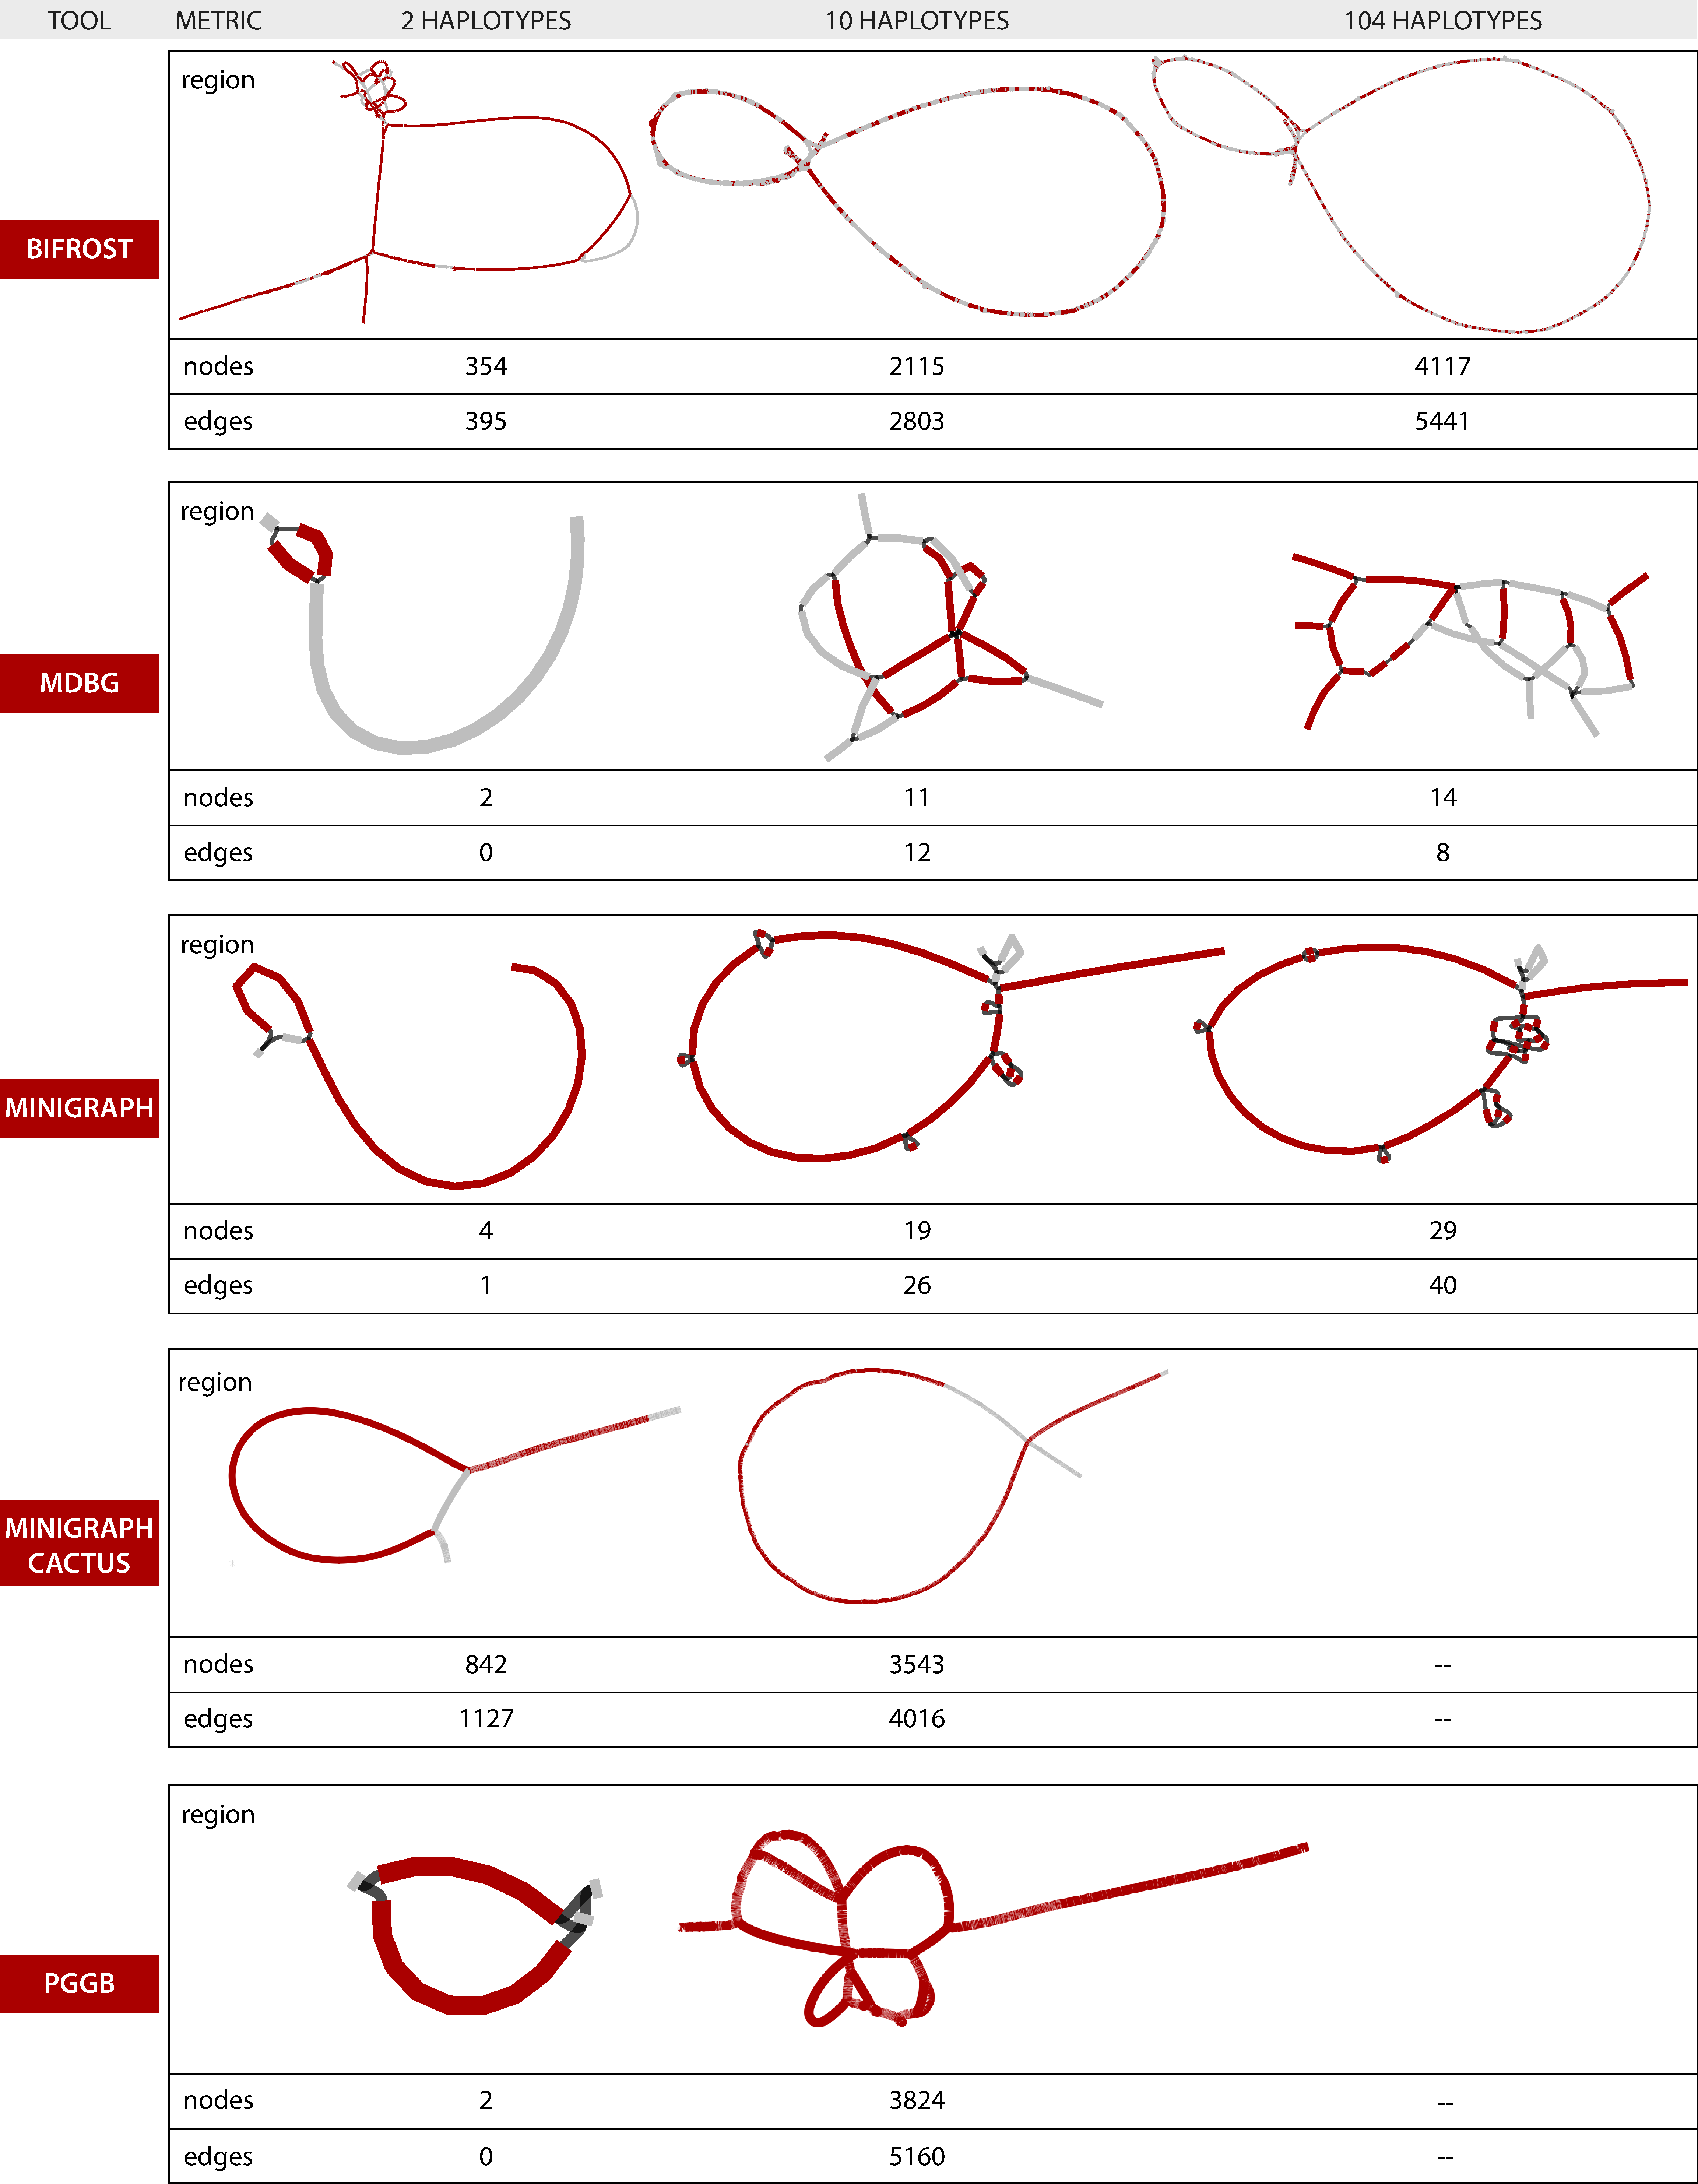
\includegraphics[width=0.95\textwidth]{figures/paperI/hla-a_corrected.pdf}
	\caption[Representations of the HLA-A locus on large human pangenomes.]{Representations of the complex HLA region by five graph construction methods over three increasing large human pangenomes. 
		See caption of Fig.~\ref{fig:HLA-E} for details. 
		%.Nodes highlighted in red are the ones that contain part of the locus sequence. The number of nodes and edges displayed represent the ones directly or indirectly attributed to the sequences that represent the locus.
	}
	\label{fig:HLA-A}
\end{figure}

\subsubsection*{\textbf{Uncovering characteristics of graphical pangenome tools}}
\label{sec:uncovering}
The data structures generated by pangenome building tools are expected to facilitate comparisons between the input genomes. In addition pangenome graphs should be stored in such a way to be easily used by downstream applications.
We identify 8 important features for pangenome graph construction tools: i) stability, ii) editability, iii) accessibility by downstream applications, iv) haplotype compression performance v) ease of visualization, vi) quality of metadata and annotation. Two other but important features, scalability and interpretability of produced graphs, were already discussed in Sections "Scalability and characteristics of pangenome graph construction tools" and "Interpretation of variation in pangenome graphs: focus on two HLA loci". %\ref{sec:scalablility} and \ref{sec:loci}. 
Table \ref{tab:tools_consideration} summarizes some of the following considerations on the relative strength of the tools.

\paragraph{\textbf{\textup{Editability and dynamic updates}}}
%\noindent\textbf{EDITABILITY AND DYNAMIC UPDATES} 
As more high quality assemblies will be generated in the near future, haplotypes may be added to a pangenome, or replaced by improved versions. Updating an existing data structure instead of rebuilding it from scratch is both computationally and energetically efficient. 
However, many succinct data structures currently used in pangenome representation are static, i.e. cannot be updated. %Current
Some methods allow a restricted set of editing operations.
\minigraph allows to add new haplotypes on top of an already built graph. \bifrost provides C++ APIs to add or remove \mbox{(sub-)sequences}, \kmers and colors from the ccdBG.
\pggb, using \odgi~\cite{odgi}, allows specific operations that delete and modify nodes and edges and add and modify paths through the graph. As \mcactus can be opened with \odgi, it supports the same operations as \pggb. 
The current \mdbg implementation uses a dynamic hash table, but does not expose an interface that supports updates.

\paragraph{\textbf{\textup{Stability}}}
%\noindent\textbf{STABILITY} 
Counter-intuitively, a pangenome graph construction tool may in some cases generate different outputs when executed multiple times with the same haplotypes as input. This \emph{unstability} could be due to a permutation in the order of the sequences given as input, or non-determinism in the construction algorithm.
Yet in order to facilitate the reproducibility of results, pangenome building tools should generate an unchanged output from the same set of input sequences, independently of the particular run or the order in which these are given.
We performed two tests to evaluate tool stability: i) we run the tools 3 times using as input the same H10 dataset and ii) we run the tools twice on shuffled input sequences, i.e. changing the order of the haplotypes of H10. 

\bifrost and \mdbg constructed exactly the same pangenome on every test, as by definition, de Bruijn graphs are stable.
\minigraph generates identical graphs on identical inputs, but generates slightly different graphs when the input is permuted. Indeed the construction algorithm of \minigraph is order-sensitive as it augments the existing graph structure by aligning the next given haplotype to it and adding divergent sequences. 
\mcactus generates slightly different graphs on identical input. 
\pggb\ generated slightly different graphs while maintaining the same haplotype sequences in the paths. The overall representation of the input genomes is therefore preserved, while the topology of the variation graph varies. The first two of the three phases of the \pggb pipeline (all-vs-all alignment and graph imputation) produce the same result on different runs with the same input but differences arise when the order of the input haplotypes changes. Most of the differences in the graph topology are thus due to the final smoothing steps.

\paragraph{\textbf{\textup{Accessibility by downstream applications}}}
% \noindent\textbf{ACCESSIBILITY BY DOWNSTREAM APPLICATION} 
\label{subs:downstream}
To facililate their adoption, pangenome representations should be easily processed by downstream analyses. 
De Bruijn graphs are challenging to analyze due to their high number of nodes, edges, and redundancy (the $k-1$-overlaps between nodes).
Though De Bruijn graph representations usually support queries of presence/absence on nodes (as in \bifrost), they lack tools able to perform more elaborate analyses such as those discussed in Section "Interpretation of variation in pangenome graphs: focus on two HLA loci", e.g. incorporating haplotype information at the \kmer level. 
On the other hand, variations graphs with paths provide more flexibility, i.e. as in \pggb and \mcactus with the \odgi visualization toolkit.
Finally in \minigraph, which considers a narrower spectrum of variants, the absence of path information prevents haplotype-level analysis; haplotypes would need to be manually mapped back to the graph. 
The choice of the pangenome building tool depends on the envisioned application. \mbox{\pggb} and \mbox{\mcactus} graphs have been shown to outperform linear references for short read mapping, genotyping and RNA sequencing mapping \mbox{\cite{hdpr}}. As these two methods  are complex pipelines based on multiple tools where parameters have been carefully set, they can be more challenging to install and run than single integrated tools. \mbox{\minigraph} alone can also be used if the focus is on structural variation instead of SNPs or small indels, and to quickly produce a pangenome graph for complex loci visualization and interpretation. The dBG-based approaches show that, for example with \mbox{\bifrost}, they retain the same base-level information as more computational-heavy variation graph approaches, but the lack of tools to use them for analysis limits their adoption.

\paragraph{\textbf{\textup{Haplotype compression}}}
%\noindent\textbf{HAPLOTYPE COMPRESSION} 
Building a graph pangenome can be seen also as a way to store, compact and retrieve the input haplotypes. As the number of new assemblies is growing faster than the data storing capacity, pangenomes can potentially help save storage space. This is highlighted by the disk space reported in Table~\ref{tab:computational_metrics}, which is consistently smaller than the sum of haplotype sizes for all methods and datasets.

In order to losslessly retrieve the input genomes from a pangenome, the  representation has to store all variations from the original haplotype sequences as paths in the graph. \pggb and \mcactus fall into this category while the other three considered tools do not store paths, or do not consider all variations, thus they are lossy.

Of note, the GBZ tool~\cite{gbz} enables graph pangenomes that store paths in the GFA file format %(the consensus file format used) 
to be stored in a lossless compressed form. It uses a Graph Burrows-Wheeler transformation to compress the graph in a more efficient way than using gzip~\cite{gbz}. Using GBZ, the pangenomes generated by \pggb and \mcactus are losslessly compressed with space gains of 3.5-5x.


\paragraph{\textbf{\textup{Ease of Visualization}}}
%\noindent\textbf{EASE OF VISUALIZATION} 
Visualizing large graphs which exceed hundreds of thousands of node is a challenge that exceeds the scope of pangenomics. The H104 pangenomes  are difficult to visualize.
Among the visualization tools considered by the Human Pangenome Reference consortium~\cite{hpp}, 
only \bandage is able to display the \minigraph or \mdbg H104 graphs, which contains a few million nodes. We reduced the number of nodes and edges of \pggb, \mcactus and \bifrost H10 graphs by collapsing isolated subgraphs representing SNPs or indels up to 10k bp (using the command \texttt{gfatools asm -b 10000 -u}). % to be able to display them. 
%Generally, general-purpose graph drawing tools able to visualize graphs with millions of nodes are needed, in particular to extract and display specific loci.

\paragraph{\textbf{\textup{Quality of Metadata and Annotation}}}
%\noindent\textbf{QUALITY OF METADATA AND ANNOTATION} 
Augmenting pangenome structures with information from other omics data would increase pangenome relevance in biological discoveries. As biobanks are rapidly growing, more data is available on regulatory regions, transcriptomics, CNVs and other medically relevant traits~\cite{100000genomes,ucla}. Pangenome data structures could leverage such information, and some of the considered tools offer basic functionality in this sense.
\bifrost provides a function to link data to graph vertices through C++ APIs. \pggb and \mcactus, using \odgi, offer annotation capabilities through insertion of paths or BED records. \minigraph and \mdbg do not offer any annotation feature. 
Specifically, in order to enhance a pangenome graph with metadata (for example with genes and regulatory regions known variants), it is desirable to maintain compatibility with methods and data formats that use a linear reference. One could conceivably project data from a graph to a reference genome to continue downstream analyses using linear coordinates. A simple method to achieve this compatibility, in our view, is to store the reference genome of interest inside the graph pangenome that supports retrieving such a reference. Variation graphs built using \mbox{\pggb or \mcactus}, due to their locally acyclical and directed construction and their use of haplotype paths, store all the coordinates needed for such a task. Haplotype paths play an important role as they avoid additional mapping to the graph, by using the \mbox{\odgi}tool to extract or inject the required information. \mbox{\minigraph} does not store haplotype paths and requires mapping sequences to the graph to restore haplotype information. On the other hand, De Bruijn graphs, using associated color data, can record the membership of k-mers to a reference sequence, yet one cannot fully reconstruct a haplotype unless k-mers positions are also stored.
\begin{table}
	\centering
	\caption[Relative strengths of five pangenome graph construction tools.]{\textbf{Relative strengths of five pangenome graph construction tools}\\
		Explanation of rows:
		1) efficacy of construction algorithm, measuring wall-clock time;
		2) degree to which variants (e.g. SNPs) are retained;
		3) ability of a tool to perform well on large datasets, both in comparison to other tools but also compared to smaller datasets;
		4) ability to modify the produced data structure to add or remove haplotypes; 
		5) property of producing the same result irrespective of perturbations, such as permutation of the input order, and repeating the same run;
		6) existence of tools (and operations) that can be applied to the resulting graphs; 
		7) whether input haplotypes information is retained by the tools, and if so, its space efficiency;
		8) whether the entire graph can be directly visualized and interpreted; 
		9) easiness of 'zooming in' a specific genomic region and interpret variants;
		10) summarizes the functionalities provided by the tools to annotate the pangenomes with genomic data;
		11) ability to share information between the graph and a linear reference.
	}
	\resizebox{\textwidth}{!}{
		\begin{tabular}{|l c c c c c|} 
			\hline
			Metric & \bifrost & \pggb & \mcactus & \minigraph & \mdbg\\
			\hline
			1) Construction speed & $\bullet\bullet\circ$ & $\bullet\circ\circ$ & $\bullet\circ\circ$ &  $\bullet\bullet\circ$ & $\bullet\bullet\bullet$\\
			\hline
			2)  Variations & $\bullet\bullet\bullet$ & $\bullet\bullet\bullet$ & $\bullet\bullet\bullet$ & $\bullet\bullet\circ$ & $\bullet\bullet\circ$\\
			\hline
			3) Scalablilty & $\bullet\bullet\bullet$ & $\bullet\circ\circ$ & $\bullet\circ\circ$ & $\bullet\bullet\circ$ & $\bullet\bullet\bullet$\\
			\hline
			4) Editability & $\bullet\bullet\bullet$ & $\bullet\bullet\circ$ & $\bullet\circ\circ$ & $\bullet\bullet\circ$ & $\bullet\circ\circ$\\
			\hline
			5) Stability & $\bullet\bullet\bullet$ & $\bullet\circ\circ$ & $\bullet\circ\circ$ & $\bullet\bullet\circ$ & $\bullet\bullet\bullet$\\
			\hline
			6) Accessibility by downstream applications & $\bullet\circ\circ$ & $\bullet\bullet\bullet$ & $\bullet\bullet\bullet$ & $\bullet\bullet\circ$ & $\bullet\circ\circ$\\
			\hline
			7) Haplotype compression performance & $\bullet\bullet\circ$ & $\bullet\bullet\bullet$ & $\bullet\bullet\bullet$ & $\bullet\circ\circ$ & $\bullet\circ\circ$\\
			\hline
			8) Ease of visualization  & $\bullet\circ\circ$ & $\bullet\bullet\circ$ & $\bullet\bullet\circ$ & $\bullet\bullet\bullet$ & $\bullet\bullet\bullet$ \\
			\hline
			9) Loci visualization and interpretability   & $\bullet\circ\circ$ & $\bullet\bullet\circ$& $\bullet\bullet\bullet$ & $\bullet\bullet\circ$  & $\bullet\circ\circ$\\
			\hline
			10) Metadata and annotation   & $\bullet\bullet\circ$ & $\bullet\bullet\bullet$ & $\bullet\bullet\circ$ & $\bullet\circ\circ$  & $\bullet\circ\circ$\\
			\hline
			11) Compatibility with a linear reference coordinates & $\bullet\circ\circ$ & $\bullet\bullet\bullet$ & $\bullet\bullet\bullet$ & $\bullet\bullet\circ$  & $\bullet\circ\circ$\\
			\hline
	\end{tabular}}
	\label{tab:tools_consideration}
\end{table}

\subsection{Discussion}
Five state-of-the-art pangenome graphs construction tools were compared on the representation of up to 104 human haplotypes. The approaches significantly differ in terms of speed, graph size, and representation of variations. We find that it remains computationally prohibitive to generate human pangenome graphs for hundreds of haplotypes, especially while retaining all variations. Each approach has its own set of strengths, and ultimately the choice of the method depends on the downstream application. In addition, several takeaway points emerged from our analysis.

First, our focused analysis of HLA loci revealed that de Bruijn graphs and variation graphs represent genomic variations equally well as pangenomes.  This is of particular importance as also shown by the draft human pangenome references~\mbox{\cite{hdpr}}: pangenomes are pivotal to trace complex and clinically relevant loci. While de Bruijn graphs are faster to construct, more stable, and scale better in terms of input size, the resulting graphs are challenging to interpret downstream. Variations graphs on the other hand are more practical to analyze at the expense of a less efficient construction step. Their visualization are more straightforward to interpret, mostly due to not having cycles, and provide insights into loci differences. 

Second, we can highlight two categories of pangenomic methods that have distinct application domains. \pggb, \mcactus and \bifrost store all possible variations, and keep haplotype information as paths or colors. They provide a complete picture of the set of variations in the input genomes which makes them difficult to analyze. They can be used for a large variety of genomic analysis, as shown for \mbox{\pggb} and \mbox{\mcactus}~\mbox{\cite{hdpr}}. \minigraph and \mdbg generate 'sketched' pangenome graphs that consider only large variants, ignoring smaller differences, and are more efficient to construct and visualize. They can be used for large scale characterization of variation in population, as proven for bacteria \mbox{\cite{mdbg}}.

Third, every tool possesses an exclusive set of features.
\pggb facilitates downstream analyses using the companion tool \odgi. It allows to precisely extract and browse any locus of interest. It is the only tool that generates variation graphs without a reference. It also keeps a lossless representation of the input sequences.
\minigraph generates a pangenome graph based on a reference sequence taken as a backbone. Its shines in the representation of complex structural variations, but does not include small or inter-chromosomal variations.
The pipeline \mcactus, that uses the \cactus base aligner, can be used to add small level variations on top of the \minigraph graph and to keep a lossless representation of the input sequences.
\bifrost illustrates that classical de Bruijn graphs are scalable, stable, dynamic, and store all variations. However, extracting information from them remain a challenge.
Lastly, \mdbg\ is the fastest construction method which generates an approximate representation of differences between haplotypes. As discussed in Section "Accessibility by downstream applications", these features enable different genomic analyses and downstream applications.

\subsection{Conclusions}
In conclusion, our results highligh the strengths and weaknesses of current pagnenome construction tools for human applications, with specific focus on how do they represent specific loci of medical relevance. We also provide insights on the features they possess and point out their best application domains.
In our view, future directions for human pangenomes building tools should focus on tackling efficiency bottlenecks, aiming to represent hundreds to thousands of haplotypes. Representations should further be lossless and represent the input haplotypes as paths in the graph. 
Such features would unlock many other applications such as lossless compression of haplotypes and cancer copy number variant analysis. 
Finally, we recognize the need for more user-friendly tools that can be used by biologists and that can translate complicated questions into  graph queries. While \odgi begins to address these questions in variation graphs, other approaches have not yet provided user-friendly interfaces. A package similar to \odgi for de Bruijn graphs would help fully realize their potential.

\subsection{Methods}
\subsubsection*{\textbf{Datasets and haplotypes collection}}
\label{sec:datasets}
In order to evaluate the state of current human pangenome representations, we sought to build a human pangenome that contains all publicly available high-quality human haplotypes. We collected from two different sources 102 different haplotypes from the genome of 51 individuals, and also used the two reference genomes, GRCh38 from the Genome Reference Consortium (GRC) \cite{grc} and CHM13 v2.0 cell line of the T2T Consortium~\cite{t2t}.
Five haplotypes correspond to Google Brain Genomics DeepConsensus \cite{deepconsensus} assembly dataset: they are hifiasm assemblies of PacBio Hi-Fi reads corrected with DeepConsensus. The average of their N50 is 37,99 Mbp. 
The remaining haplotype assemblies as well as the T2T reference are from the Human Pangenome Reference Consortium (HPRC) year-1 freeze~\cite{hpp}, and GRCh38 is from the GRC. Their average N50 is 40.3 Mbp. Since HG002 is contained in the DeepConsensus data, the HPRC HG002 haplotypes were not used.
The origin and the sex of the individuals are diverse %to aim for a 
and provide a fair representation of the diversity in human population: out of 51 total individuals, 21 are males and 30 are females and they represent 14 different ethnic groups, from US to Africa and Asia. We did not perform any additional selection, regarding sex and ethnicity, on these public datasets as our main goal was to use as many genomes as possible. However, the HPRC stated that the genomes were selected to represent genetic diversity in humans~\mbox{\cite{hdpr}}.

To evaluate the scalability of pangenome construction tools, we created three datasets of increasing size: 1) 2 haplotypes from the same individual, HG006, 2) 10 haplotypes from 5 different individuals (HG002, HG003, HG004, HG006 and HG00735) and finally 3) all of the 104 haplotypes. To test whether the order of the input sequences matters, we considered various random orderings for the 10 haplotypes in Dataset 2. Since \minigraph needs a reference sequence as fist haplotype in order to correctly build the graph, we generated specific 2 and 10 haplotypes datasets with the first haplotype replaced by the reference genome CHM13. This was applied to the \mcactus pipeline as well as it uses \minigraph variation graphs.

\begin{table}
	\centering
	\setlength{\tabcolsep}{5pt} 
	\caption[Description of the three datasets generated to test the scalability of the tools.]{\textbf{Description of the three datasets generated to test the scalability of the tools}
		\\
		Data sources: 
		$^1$ Google Brain Genomics~\cite{google-assemblies}; $^2$ Human Pangenome Reference Consortium~\cite{HPRC-haplotypes}; $^3$ 1000 Genomes Project~\cite{HPRC-haplotypes}; $^4$ Telomere to Telomere Consortium~\cite{HPRC-haplotypes}.
		\label{tab:datasets}}
	\renewcommand{\arraystretch}{1.2}
	\begin{tabular}{|c c c|}
		\hline
		\centering
		Haplotypes & Project & Bases \\
		\hline
		2 & Google$^1$ & 5.9 Gbp\\
		10 & Google, HPRC$^2$ & 30 Gbp \\
		104 & Google, HPRC, 1KG$^3$, T2T$^4$ & 313.6 Gbp \\
		\hline
	\end{tabular}
\end{table}

\subsubsection*{\textbf{Pangenome graph construction tools}}
\label{sec:tools}

We evaluated tools that generate graph pangenomes as variation graphs and colored compacted de Bruijn graphs. Variation graphs are generally locally acyclic while de Bruijn graphs have cycles. In variation graphs, nodes represent sequences and edges represent immediate sequence adjacency without overlap. Variation graphs are generally easier to visualize and to interpret while challenging to construct at scale and, apart from \pggb, require a reference genome. In de Bruijn graphs (\dbg), nodes are \kmers (string of length k) and edges are (k-1)-overlaps between nodes. In practice, \dbgs are represented in a compact way where all nodes along unbranching paths are compacted into \emph{unitigs}. The resulting graph is called compacted De Bruijn Graph, where nodes are unitigs and edges represent (k-1)-overlaps. 
As shown in Figure \ref{fig:figure1}, de Bruijn graphs %are easier to construct and are more standardized but 
result in large graphs that pose visualization and interpretation challenges, in particular as there is no alignment to a reference.

\begin{itemize}
	\item
	\bifrost constructs dynamic, coloured compacted de Bruijn Graphs (\emph{\ccdbg}). It first generates a standard \dbg using an efficient variant of Bloom Filters and then computes the compacted \dbg from it.
	Colors, i.e. identifiers representing the sample origin of each k-mer are added by storing an array per \kmer. A human genome \ccdbg typically consists of a single large connected component, as common \kmers are shared between chromosomes. This pangenome representation contains all the variations present in input sequences.
	
	\item
	\mdbg builds a variant of de Bruijn graphs called a minimizer-space de Bruijn Graph (\mdbg), which is efficient to construct as it only considers a small fraction of the input nucleotides. Color information is currently not supported in the implementation. Similarly to Bifrost, a \mdbg also typically represents a human genome as a single large connected component, albeit with orders of magnitude less nodes. Minimizer-space de Bruijn graphs mostly discard small variants, yet are sensitive to heterozygosity which creates branches in the graph.
	
	\item
	\minigraph constructs a directed, bidirected and acyclic variation graph iteratively by mapping new haplotypes using a combination of the minimap2 tool and the graph wavefront alignment algorithm. The first input sequence acts as a  backbone for the whole representation.
	The sample(s) of each node are stored in a rGFA output file.
	\minigraph considers only variations longer than 50 bps hence it is oblivious to isolated SNPs and small indels: even if it produces base-level alignment for contigs, the graphs are not a base-level resolution. The resulting graph is divided into connected components that correspond to the chromosomes present in the first given input genome.
	%, yet can represent large divergent regions at base-pair resolution
	\item
	\mcactus is a variation graph construction pipeline that combines \minigraph to generate a structural variations graph and \cactus base aligner to generate base-level pangenome graphs of a set of input assemblies and embg: The definition of \label has changed! Check your packages! Replacing it with the kernel definition on input line 145.ed haplotypes paths. \cactus~\cite{cactus} is a highly accurate and scalable reference-free multiple whole-genome alignment tool, that in this pipeline considers the reference sequence used by \minigraph to ensure that the resulting variation graph is acyclic. The final graph is further normalized using GFAffix\cite{gfaffix}. The pipeline allows to generate multiple graphs, one for each chromosome, or produce a single graph that includes inter-chromosomal variants.
	
	\item
	\pggb is a directed acyclic variation graph construction pipeline rather than a single tool. It calls three different tools: pairwise base-level alignment  of haplotypes using wfmash \cite{wfmash}, graph construction from the alignments with seqwish \cite{seqwish}, graph sorting and normalization with smoothxg and GFAffix \cite{smoothxg,gfaffix}.
	The resulting variation graph represents variations of all lengths present in the input sequences.
\end{itemize}


\begin{table}
	\centering
	\caption[URL, version, pangenome representation and parameters of the three analyzed tools.]{ \textbf{URL, version, pangenome representation and parameters of the three analyzed tools.}\\ pggb/0.2.0 used wfmash v0.7.0, seqwish v0.7.3 and smoothxg v0.6.1.}
	\resizebox{\textwidth}{!}{
		\begin{tabular}{|c c c c c|} 
			\hline
			Tool  &  Github repository & Graph type & Version & Parameters \\ 
			\hline \hline
			\bifrost & pmelsted/Bifrost  & De Bruijn graph  & 1.0.5 & -k100 -c \\ 
			\hline
			\pggb &   pangenome/pggb & variation graph  & 0.2.0 & -p 98 -s 10000 -k 311 -G 13033,13117\\ &&&& -O 0.03 -v -t 8 -T 8 -A -Z \\ 
			\hline
			\minigraph & lh3/Minigraph  & variation graph &   0.18 & -cxggs\\ 
			\hline
			\mcactus & ComparativeGenomics  & variation graph &   2.2.3 & --maxLen 10000 --delFilter 10000000 \\ & Toolkit/cactus &&&\\ 
			\hline
			\mdbg  & ekimb/rust-mdbg  & De Bruijn graph &  1.0.1 & -k 10 -d 0.0001 --minabund 1 --reference\\ 
			\hline
	\end{tabular}}
	\label{tab:url}
\end{table}



\subsection*{Supplementary Information}

\subsubsection*{\textbf{Benchmark infrastructure}}

Running time of pangenome construction tools was measured as wall clock time and peak memory as maximum resident set size using the \texttt{time} command. Other metrics were obtained with custom Python scripts. All benchmarks were performed on a Supermicro Superserver SYS-2049U-TR4, with 3 TB RAM and 4 Intel SKL 6132 14-cores @ 2.6 GHz, using 8 cores. \\

\subsubsection*{\textbf{TwoPaCo}}
\label{app:twopaco}
We did not consider \twopaco as it is redundant with \bifrost. Both methods construct the same de Bruijn graphs.
\twopaco is a method for constructing \ccdbgs by finding junction \kmers at the boundaries of unitigs or in branching nodes. It consists of two main steps in which it approximates the dBG with a Bloom filter in order to reduce the size of the problem and then runs a two pass highly parallel algorithm on it. It constructs ccdBGs similarly to \bifrost. \bifrost  is faster, supports edit operations, and accepts also reads other than assemblies as input. We tested both tools on NCBI datasets from three different known human variation regions part of the human leukocyte antigen (HLA) complex: HLA-A, MICB and TAP1. These loci have different number of sequences and have complexity and length. The resulting graphs have exactly the same k-mer content and substantially equal topology. The difference is that \twopaco considers sequences with IUPAC 'N' bases while \bifrost does not and that in some cases \twopaco renders some unitigs split in two or more consecutive nodes.

\subsubsection*{\textbf{Loci extraction method}}
\label{app:extraction}
For \bifrost and \mdbg graphs, nodes corresponding to the input sequences are identified with \graphaligner\cite{graphaligner} and the subgraph is extracted using the \bandage \emph{reduce} function. As the aligned nodes are not expected to represent the full diversity of the population in the pangenomes, the considered portion of the graph contains also nodes up to a certain distance from the aligned ones: 1 for \mdbg and 3 for \bifrost. This number is based on the size of the sequences spelled by the nodes and on the considered variations. Artifacts, mostly tips, that are not part of the locus of interest are removed with a custom python script. For \minigraph generated graphs, the \minigraph own alignment function has been used to identify the nodes and then \bandage is used to extract the subgraph. For \pggb, first we generate a bed file of the position of the region of interest in every haplotype used to construct the graph. The ranges are derived from aligning them to the locus sequence(s) using minimap2 \cite{minimap2}. The graph corresponding to the region is then extracted using the \odgi extract and \odgi view functions. For \mcactus we use the same strategy as \pggb, with the difference that the bed file is only for the reference CHM13, present in the graph. \\
The annotation of the specific loci in the subgraph is done using nodes from the alignment with \minigraph or \graphaligner to the subgraph. This makes it possible to highlight multiple sections in the region, as, for example, genes and pseudogenes of interest. 

\subsection*{\textbf{Availability of data and materials}} %Reproducibility and Data Availability
The scripts used to generate and analyse the pangenomes can be found at \cite{source-code-github}\cite{source-code-zenodo} under MIT license.
Google Brain Genomic assemblies can be found at \cite{google-assemblies}. \\
HPRC assemblies, CHM13 and GRCh38 can be found at \cite{HPRC-haplotypes}.

\subsection*{\textbf{Funding}}
R.C was supported by ANR Full-RNA, SeqDigger, Inception and PRAIRIE grants (ANR-22-CE45-0007, ANR-19-CE45-0008, PIA/ANR16-CONV-0005, ANR-19-P3IA-0001). This project has received funding from the European Union’s Horizon 2020 research and innovation programme under the Marie Skłodowska-Curie grants agreements No. 872539 and 956229.

\subsection*{\textbf{Author's contributions}}
FA, YD and RC conceived and designed the project. FA implemented the scripts. FA and PL ran the experiments. FA, YD, PL and RC wrote the paper. The authors read and approved the final manuscript.

%% Format bibliography like a section, not a chapter:
% \printbibliography[heading = subbibliography]
% \stopcontents[chapters]© Francesco Andreace, 2024

Series of dissertations submitted to the
Insitut Pasteur Paris, Universite’ de Paris Cite, University of Oslo
No. 1234
ISSN 1234-5678
All rights reserved. No part of this publication may be
reproduced or transmitted, in any form or by any means, without permission

\paragraph{Authors' affiliations}
\begin{description}
	\item[Francesco Andreace]
	Institut Pasteur, Université Paris Cité, G5 Sequence Bioinformatics \\
	Sorbonne Université, Collège doctoral \\
	25-28 Rue du Dr Roux, 75015 Paris
	
	
	\item[Pierre Lechat]
	Bioinformatics and Biostatistics Hub, Institut Pasteur, Université de Paris Cité \\
	25-28 Rue du Dr Roux, 75015 Paris
	
	\item[Yoann Dufresne]
	Institut Pasteur, Université Paris Cité, G5 Sequence Bioinformatics \\
	Bioinformatics and Biostatistics Hub, Institut Pasteur, Université de Paris Cité \\
	25-28 Rue du Dr Roux, 75015 Paris
	
	\item[Rayan Chikhi]
	Institut Pasteur, Université Paris Cité, G5 Sequence Bioinformatics \\
	25-28 Rue du Dr Roux, 75015 Paris
\end{description}
%\stopcontents[chapters]
\newpage

\subsection{Perspectives}
The results of the work outlined in this section suggest several directions for future investigation and software development: they can be divided into a few axes.
On one side, the scripts and software that I developed to produce the analysis of this paper could have been extended into an automatic reproducible pipeline. By integrating the code into platforms like nextflow or Snakemake, this could become a benchmark for current and future pangenome tools, as, at the moment, there is no other way to independently compare the output of tools that produce variation graphs and \dbgs. \\
On another side, there are many more features that could be added to the analysis workflow to produce a more in-depth and accurate description of the resulting pangenomes, like node (sequence) length distribution, node degree distribution, count of SNPs and indels. It is important to stress that detection of specific patterns of variation is non-trivial in data-structures like \dbgs. Finally, another experiment that could be done is to convert, using path information, the variation graph into a \ccdbg, to compare against a \ccdbg built directly from the input sequences: this would allow to verify if the information stored into the two data structures is equivalent. \\
Another very interesting avenue would be to develop a tool that enables complex information extraction from \ccdbgs. Construction tools usually offer commands or APIs to perform simple absence/presence queries, that are mostly useful when they are used for metagenomic purposes but offer less actionable insight in pangenomics analysis. An idea that I have started exploring during this PhD is to extract a subgraph of a \ccdbg that represent a locus or gene of interest in the whole dataset provided as input. \\ 
Finally, it would be very useful to define a \ccdbg output color format that every tool should also use to output the colors, like gfa is used to output graphs. As of now, each tool implements its own binary format for color storage, discouraging downstream analysis software development, as it would be bound to specific construction tools and not the common data structure used.

\newpage

\section{Building a \emph{Lodderomyces elongisporus} pangenome reference: overcoming current limitations.}
We present another example of extending variation graph pangenome building strategies, specifically in producing a graph that can represent inter-chromosomal events, such as rearrangements, for the medically relevant yeast strain of \lodelo.We also demonstrate how a pangenome-based approach can provide more comprehensive insights into such events compared to a linear genome-based approach.\\
he work presented here is partially a collaborative effort with other PhD students and researchers, co-led by Daniel Doerr and myself during a winter school organized by our consortium. I would like to acknowledge Simon Heumos for our discussions on the construction of such graphs, and Nicola Rizzo. The majority of the results and findings reported here are primarily my own subsequent work.\\
The following sections will explain the process required to produce custom, biologically significant, and biologically driven pangenome graphs of a yeast strain using current state-of-the-art tools. We will offer insights into workarounds that can be employed in cases with special requirements, where current tool features limit the analysis that can be performed. This will also demonstrate how pangenome models can offer more powerful tools for analyzing specific variations in a group of similar genomes compared to linear reference-based models.\\ 
In this specific case, the goal was to produce a variation graph that represents the long chromosomal translocations observed by the team that produced the assemblies from short and long reads. Chromosome-crossing syntenies for multiple contigs in alignment hits of chromosomes C, G, and H were detected, suggesting that they could correspond to a single recombination group. This finding was consistent with an independent SNP-based genomic study performed on isolates from a fungemia outbreak in a neonatal intensive care unit in Delhi between 2021 and 2022. The study noted that these translocation events are more frequent in hospital and patient-associated populations than in fruit-associated populations~\cite{lodelo_india}. \\
In summary, the work here presented will be organized as follows:
\begin{enumerate}
	\item Brief characterization of \lodelo genome and relevance;
	\item Pangenome graphs constructed and their utility;
	\begin{enumerate}
		\item Determining the chromosomal communities from the assemblies to generate a variation graph of interest;
		\item Producing a variation graph with \pggb;
		\item Producing a variation graph with \mcactus by customizing the pipeline and the data;
	\end{enumerate}
	\item Representation of translocation events in variation graphs;
\end{enumerate}

%By plotting the alignments of the 2 best quality assemblies, B2 and J2, for chromosome C,G and H, shown in figure~\ref{fig:lodelo_dotplot-alignments}.
%\begin{figure}[t]
%	\centering
%	\begin{subfigure}[b]{0.46\textwidth}
%		\centering
%		\includegraphics[width=.95\linewidth]{figures/lodelo/map_BG_JG.png}
%		\caption{Alignment between chromosome G of B2 and J2.}
%	\end{subfigure}%
%	\begin{subfigure}[b]{0.46\textwidth}
%		\centering
%		\includegraphics[width=.95\linewidth]{figures/lodelo/map_BH_JG.png}
%		\caption{Alignment between chromosome H of B2 and chromosome G J2.}
%	\end{subfigure}
%	\begin{subfigure}[b]{0.46\textwidth}
%		\centering
%		\caption{Alignment between chromosome C of B2 and J2.}
%	\end{subfigure}
%	\begin{subfigure}[b]{0.46\textwidth}
%		\centering
%		\includegraphics[width=.95\linewidth]{figures/lodelo/map_BC_JH.png}
%		\caption{Alignment between chromosome C of B2 and chromosome H of J2.}
%	\end{subfigure}
%	\caption{Dot-plot of the mapping of the resolved chromosomes of samples B2 and J2 for chromosomes C,G and H using D-Genies~\cite{dgenies} shows how large chunks of DNA is harbored into different chromosomes depending on the sample. Alignments were obtained using \wfmash \texttt{-p90 -s10000}.}
%	\label{fig:lodelo_dotplot-alignments}
%\end{figure}

%The consortium my phd fellowship belongs to, the EU Commission founded Marie Curie ITN Alpaca (Algorithms for Pangenomic computational analysis) consortium~\cite{alpacawebsite}, organized a winter wet-lab school to give a small training on how the processing of preparing samples for sequencing works, in order to improve the knowledge on the full stack of processes done to obtain genomes from biological samples of the medically interesting yeast strain of \lodelo. From 11 different samples, we generated long (ONT) reads, in collaboration with a lab at the Comenius University in Bratislava, Slovakia. We divided into several groups to perform different genomic analyses on it. One of these team, the one I was in, was tasked on building a pangenome reference of \lodelo. \\ 
%We sequenced,  The computational work I present here was done in collaboration with members of the consortium, in large part by Simon Heumos, whom I would like to thank for the time spent discussing and working together.

\subsection{\emph{Lodderomyces elongisporus}: genetic characteristichs, interest and used data}
\emph{Lodderomyces elongisporus} is a diploid yeast that has been isolated from, among many sources, humans and it is recently emerging as pathogenic. It is phylogenetically placed in the Candida clade and the size of its genome is usually between 15 and 16 Mb, 2 orders of magnitude smaller than a human genome~\cite{Lodderomyces}. Its DNA is organized into 8 chromosomes, that here will be referred in alphabetical order and decreasing size A to H, from around 3.5Mbp of chr A to 800 Kbp of chr H, plus a 35 Kbp mitochondrial DNA. Our analysis shows that it has a stable core genome of ~13Mbp, as shown in section~\ref{sec:core_pg}. 
Increasing reports of (mostly bloodstream) infection in mainly immunosuppressed adults makes it an increasingly important subject of studies\cite{lodelo_pathogen,lodelo_fatal,lodelo_meningitis,lodelo_bloodstream}: it also got recent attention when an outbreak was reported occurring in a neonatal ICU in Dheli, India from September 2021 to February 2022 with 1 death\cite{lodelo_india}.\\
11 samples sequenced by us were assigned names with one letter in alphabetical order from A to K followed by a number greater or equal than 0 that denoted the quality of the assembly (with 0 draft to 2 maually curated). More in depth statistics like the number of sequences, N50 and others are shown in table~\ref{tab:assembly_stats}. Moreover, one sample, B2, for which a member of the consortium produced a high quality assembly after intensive manual curation, was used as relative reference in the cohort. Another sample, J2, was also fully resolved into chromosomes while the others were assembled into contigs.
\begin{table}[h!]
	\centering
\rotatebox{90}{
	\begin{minipage}{1.55\textwidth}
	\centering
\begin{tabular}{| c | c | c | c | c | c | c | c | c | c |}
		\toprule
		sample     &   tot length (bp)  & sequences & mean length & longest seq & shortest seq &   N count & Gaps &   N50  &   N50n  \\
		\midrule
		A1 & 15699113 & 25 & 627964.52 & 2595744 & 3907 & 0 & 0 & 1354781 & 5  \\
		B2 & 15485469 & 9 &  1720607.67 & 3516991 & 35166 & 0 & 0 & 2266654 & 3 \\
		C0 & 15532065 & 20 & 776603.25 & 3532941 & 810 & 0 & 0 & 1331232 & 4  \\
		D0 & 15507665 & 17 & 912215.59 & 3532853 & 5008 & 0 & 0 & 2160581 & 3 \\
		E0 & 15332588 & 18 & 851810.44 & 3544471 & 3228 & 0 & 0 & 1992182 & 3  \\
		F1 & 15664073 & 21 & 745908.24 & 3548518 & 1282 & 0 & 0 & 2165076 & 3 \\
		G0 & 15636520 & 19 & 822974.74 & 3548910 & 550 & 0 & 0 & 1697956 & 4  \\
		H0 & 15601346 & 21 & 742921.24 & 3549008 & 6842 & 0 & 0 & 2170489 & 3 \\
		I1 & 15639882 & 30 & 521329.40 & 3622524 & 536 & 0 & 0 & 1999295 & 3 \\
		J2 & 15425942 & 9 & 1713993.56 & 3543738 & 35442 & 0 & 0 & 2157297 & 3 \\
		K0 & 15752744 & 16 & 984546.50 & 3534745 & 19835 & 0 & 0 & 1631500 & 4  \\
		\bottomrule
	\end{tabular}	
	\caption[\lodelo samples assembly statistics]{\lodelo samples assembly statistics. N50n represents the number of sequences that contain 50\% of the assembly.\\ There are no unknown nucleotides or gaps (any arbitrary stretch of Ns - i.e. unknown nucleotide). Metrics obtained using assembly stats software from Sanger Institute~\cite{assemblystats}.}
	\label{tab:assembly_stats}
	\end{minipage}}
\end{table}
\subsection{Building ad hoc pangenome reference}
We produced a \dbg from all 11 assemblies described in table~\ref{tab:assembly_stats} using \bifrost, but their usefulness remains limited for visual analysis of complex biological events interpretation and study.\\
Figure~\ref{fig:lodelo_dbg} shows the visualization of the \dbg for \kmer length equal to 25: repetitions make the visualization of the graph challenging. This is the same phenomenon previously described for human genomes, as better insight can be acquired when just a small region is visualized. 
De Bruijn Graphs can instead be useful to produce quite straightforward whole-genome alignment-free and reference-free phylogenetic analysis in a fraction of time required by competitor methods that use all vs. all alignment. The tool \sans~\cite{sans} can process directly a \bifrost generated \ccdbg to estimate the phylogenetic splits between the genomes contained in the graph. Figure~\ref{fig:dbg_phyl} shows the visualization of the phylogenetic network produced by \sans using the tool \splitstree~\cite{splitstree}. By adding another genome from a close species it is possible control that the \dbg-based analysis provides results compatible with expectations. Figure~\ref{fig:beig_phyl} shows the phylogenetic network when an assembly of \emph{Lodderomyces Beijingensis} is added to the graph: the new genome is very separated compared to the other ones from the same species. This results shows how \dbgs are a powerful model when applied to specific applications.\\

\begin{figure}[h]
	\centering
	\includegraphics[width=1\linewidth]{figures/lodelo/lodElo_k25.png}
	\caption{\bandage visualization of the pangenome \dbg of the cohort of 11 \lodelo strains. As for human genomes, visualization of the whole data offers no particular insight, apart from the large variations visible on the rounded parts away from the dense part.}
	\label{fig:lodelo_dbg}
\end{figure}%

\begin{figure}[h!]
	\centering
	\begin{subfigure}[b]{\textwidth}
		\centering
		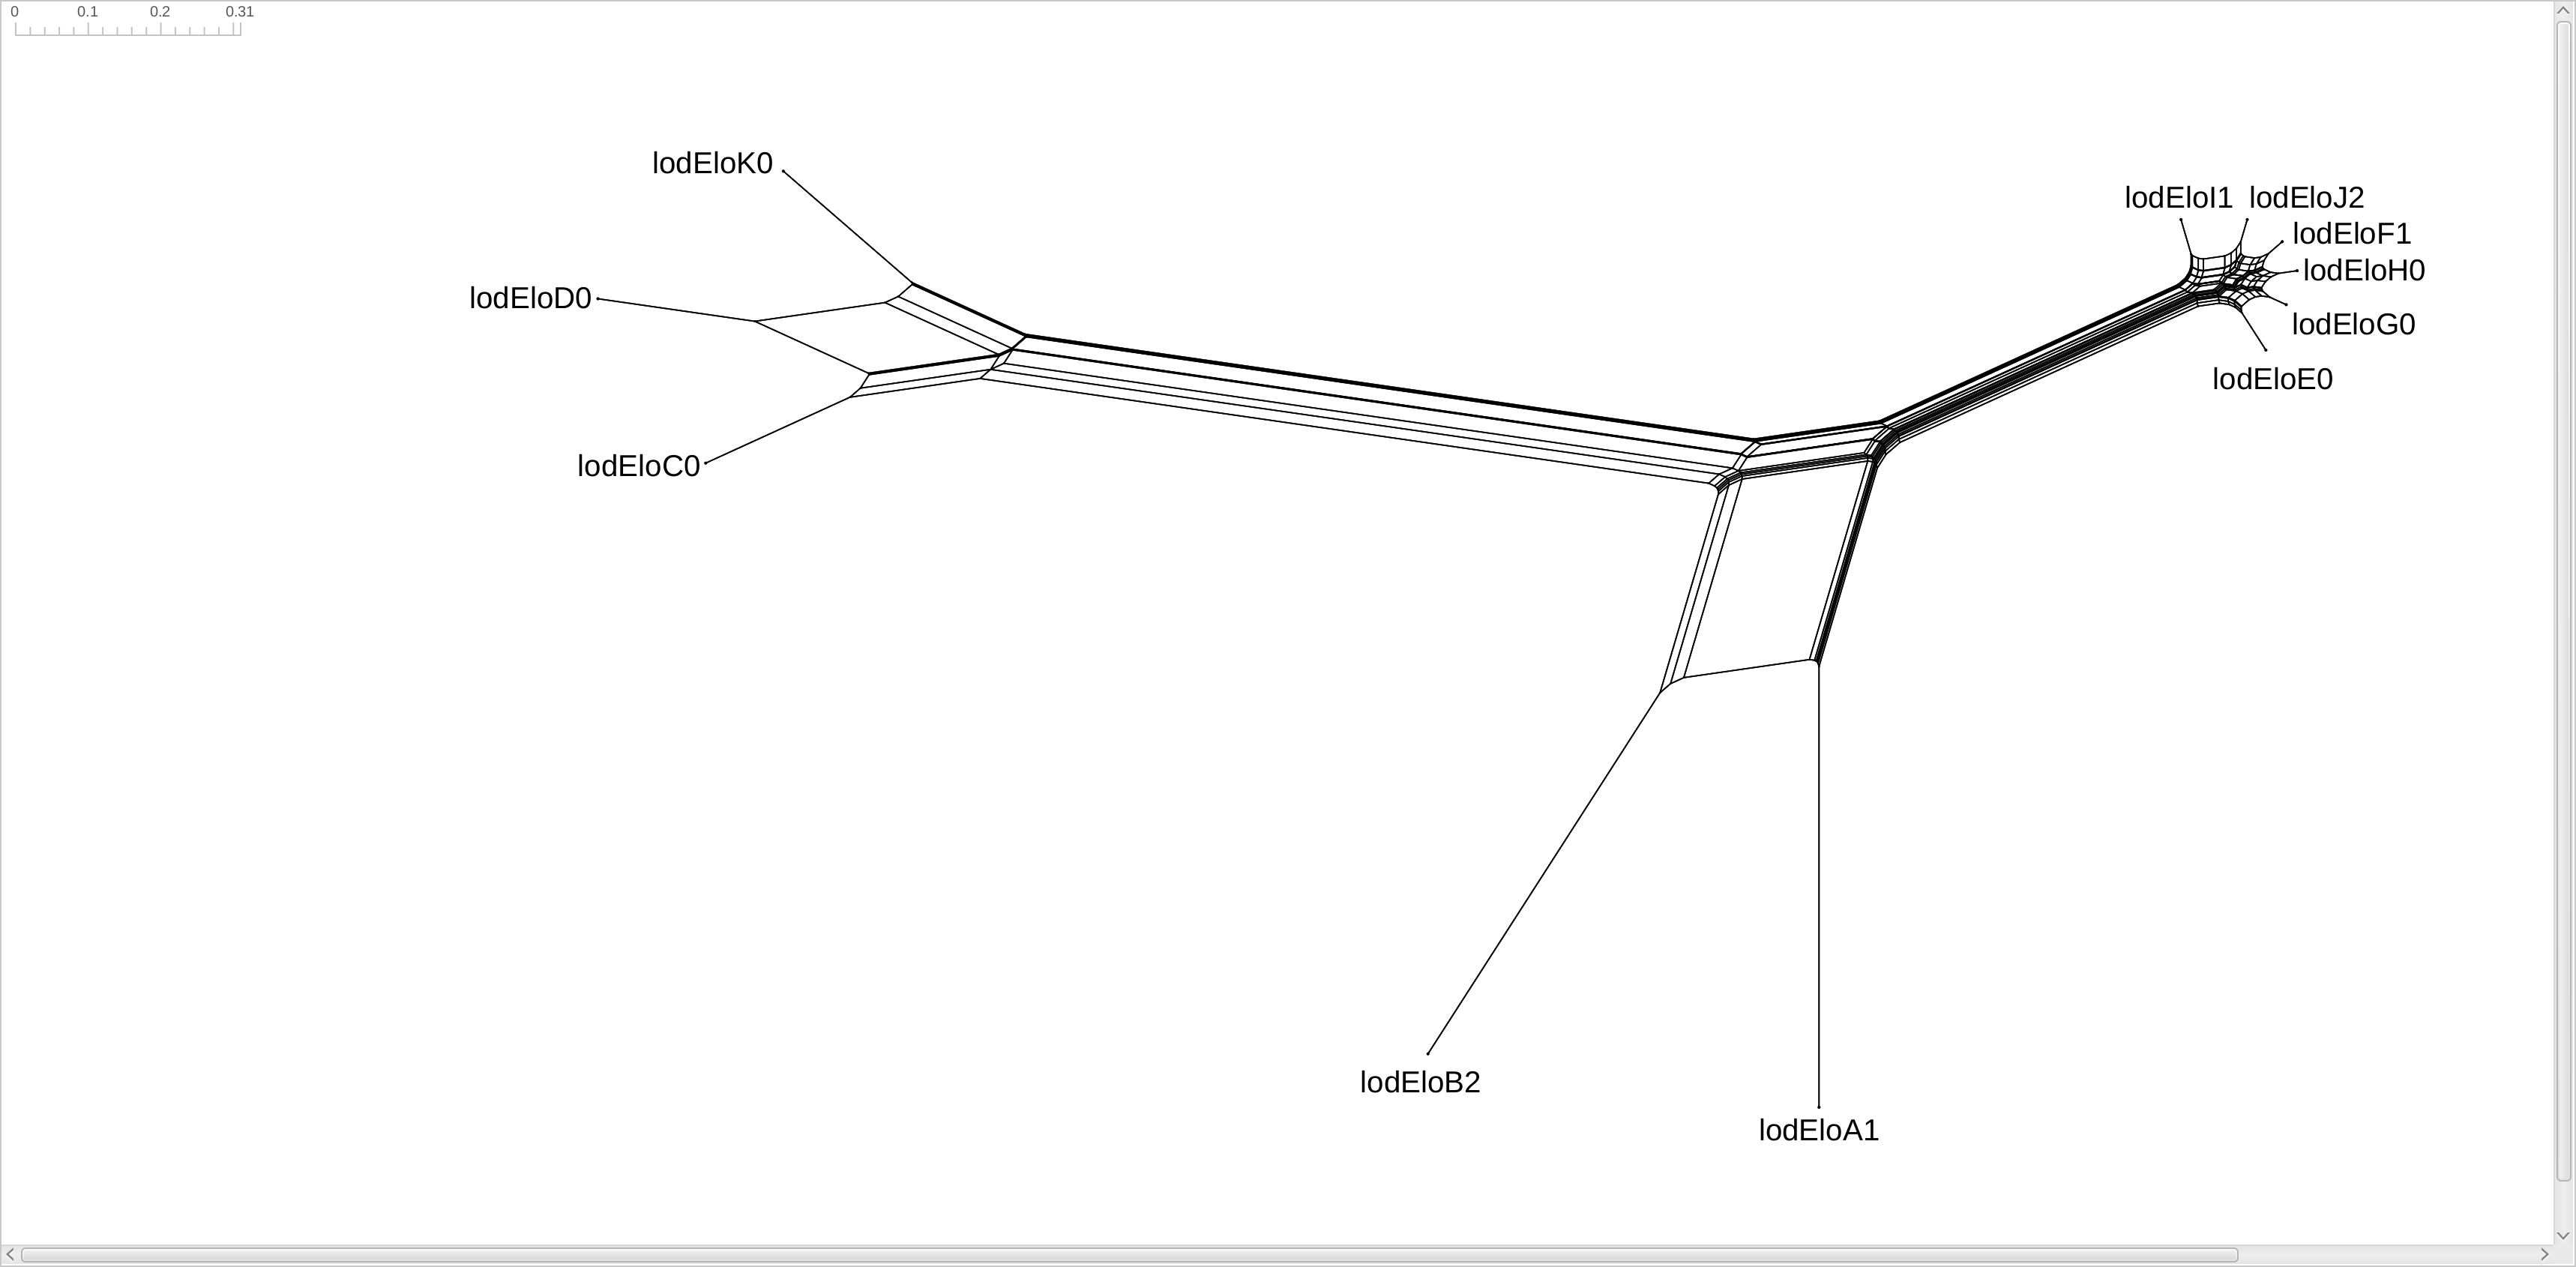
\includegraphics[width=1\linewidth]{figures/lodelo/direct_nobei.png}
		\caption{\splitstree visualization of the phylogeny network generated using \sans from the \ccdbg constructed using \bifrost.}
		\label{fig:dbg_phyl}
	\end{subfigure}%
	\\
	\begin{subfigure}[b]{\textwidth}
	\centering
	\includegraphics[width=1\linewidth]{figures/lodelo/lodelo_bei.png}
	\caption{Phylogeny network of the 11 \lodelo strains plus one genome of \emph{Lodderomyces Beijingensis} shows the ladder separated on the right while the group of subfigure b compacted on the left. As they are two different species, although close in the Candida/Lodderomyces clade\cite{lodelo_genomes}, this result provides positive control for the phylogeny network generated using \sans from the \ccdbg constructed using \bifrost. This image was produced by Nicola Rizzo.}
	\label{fig:beig_phyl}
	\end{subfigure}%
	\caption[\ccdbg representation and phylogeny analysis of the \lodelo pangenome.]{Visualization of the \ccdbg representation and phylogeny analysis of the \lodelo pangenome.}
\end{figure}
Given high quality assemblies generated by the sequences of these 11 samples, we decided to also build a pangenome graph with small variant resolution using \pggb and \mcactus, in a similar way to what has been done with the Human Draft Pangenome Reference~\cite{hdpr}. In order to produce a graph with a structure that resembles biologically expected variation structures, several rounds of parameter tuning and manual curation are needed, with knowledge which is out of reach from inexperienced users.\\
The first step to build such pangenomes is to divide the genome assemblies into communities of sequences belonging to chromosomes.

%As explained before, variation graphs generation is given by communities separation. \pggb works by building a single graph from a given community, so it fits well for this specific use-case: by grouping together the contigs corresponding to the three chromosomes where the recombination occurred, the pipeline should produce a graph that consider this event.
\subsubsection{Determining chromosomal communities}
Variation graphs construction pipelines use mapping or alignment between the input set of genomes to infer graphs. Their first step consists in grouping the sequences from the assemblies into communities representing a chromosome in order to run a single computation instance and produce a separate graph for each of them. The final graph is then obtained by joining together the output of each group. This means that without any pre-processing, no inter-chromosomal event can be detected.\\ 
In this specific use-case, in order to identify inter-chromosomal events, contigs associated to any of the 3 chromosomes conjectured to be part of the rearrangement had to fall into the same community and be provided together in input to the pipeline. This would ensure that, if such rearrangement exists, it would produce a feature in the graph that would show as a tangle between the chromosomes.\\
As the rest of the assemblies, with the exception of the J2 sample, were not resolved into single chromosomes, each of them was aligned to the reference B2 using \wfmash alignment segment size of 10k and 95\% sequence identity (and lower segment size, 90\% sequence identity if unmapped). The identity scores of the alignment of the genomes to the reference B2 assembly is shown in figure~\ref{fig:lodelo_alignment_scores}. From this alignment, contigs were assigned to the chromosomal community to which they best mapped. Finally, contigs assigned to chromosomes C,G,H were grouped manually into a single community.
\begin{figure}[h!]
	\centering
	\includegraphics[width=.8\linewidth]{figures/lodelo/Alignment_scores.pdf}
	\caption[Sequence Identity of \lodelo samples's contigs assigned to reference chromosomes.]{Sequence Identity of contigs assigned to reference chromosomes. Image produced using a pipeline developed by Simon Heumos.}
	\label{fig:lodelo_alignment_scores}
\end{figure}

\subsubsection{Producing a variation graph using pggb}
As \pggb uses all-vs-all alignment of a collection of sequences as first step to infer the graph, it enables the representation of recombination among chromosomes placed inside the same community, as seen also for human acrocentric chromosomes~\cite{Guarracino2023}.\\
The \texttt{nextflow/pangenome} (\pggb) pipeline was run for each of the identified chromosomal communities to produce a first pangenome representation of the 11 yeast strains. The tangle visible in figure~\ref{fig:lodelo_gfaestus} clearly shows the recombination happening between the three chromosomes. This work was mainly done by Simon Heumos and the graph shown in figure ~\ref{fig:lodelo_gfaestus} is the result of more than 25 rounds of parameters tuning.
The detection of the event with a variation graph using \pggb encouraged the effort to produce a similar representation with \mcactus, a pipeline that is not designed to construct grouped chromosomes pangenomes. The goal was to double check with another pangenome construction software the structure of the translocation in the pangenome graph.
\begin{figure}[h!]
	\centering
	\includegraphics[angle=90,width=.6\linewidth]{figures/lodelo/pggb_full.png}
	\caption[\gfaestus visualization of a \lodelo variation graph.]{\gfaestus visualization of the \pggb variation graph of the 11 \lodelo samples. Image produced by Simon Heumos.}
	\label{fig:lodelo_gfaestus}
\end{figure}


\subsubsection{Overcoming \mcactus limitation by modifying both the data and the pipeline}
In order to produce a graph that represents variation between multiple chromosomes with \mcactus, a custom pipeline has to be used. \mcactus communities are implicitly inferred by the first step, performed by \minigraph. For this tool, the chromosomes present in the first reference genome given as input are used as communities and backbone for the whole graph and no sequence can be both assigned to different chromosome. This is an intrinsic characteristic of \minigraph and cannot be changed with input parameters: it means that there is no feature to have chromosome C,G and H considered together in input.\\
To try to overcome this limitation of the approach we tried to produce a graph that respected the condition of having the three chromosome inside the same connected component, at the cost of producing a representation that was not biologically correct. We therefore produced a chimeric contig consisting of the concatenation of the three chromosomes assemblies of the B2 sample. The rationale was to provide the 3 chromosomes chained together as a single backbone in the \minigraph construction step. This would allow sequences to be mapped to any of chr C, G and H to be considered together in the subsequent steps of alignment and graph the \mcactus pipeline. The expectation was to therefore produce a graph that showed the recombination from the mapping of the contigs of the other genomes. \\
We generated a graph using \minigraph with the chimeric chromosome CGH and all the contigs of the other genomes assigned to chromsome C, G and H. As shown in figure~\ref{fig:cgh_mingraph}, it does not represent any recombination event. This was somewhat expected, as it is known that \minigraph does not also consider inversion between genomes.
When the pipeline of \mcactus is run using by chromosome communities, with the chimeric chromosome CGH and its assigned contigs as a single community, it is possible to see the tangle between the chromosomes, as shown in figures~\ref{fig:cgh_mcactus}~\ref{fig:lodelo_graph_tangle}.
\begin{figure}[h!]
	\centering
	\begin{subfigure}[b]{\textwidth}
		\centering
		\includegraphics[width=.8\linewidth]{figures/lodelo/minigraph_cgh.png}
		\caption{Graph of chimeric chromosome CGH from sample B2 and all the contigs of the other genomes aligning to it produced with \minigraph. The graph is linear and no inter-chromosomal event is visible.}
		\label{fig:cgh_mingraph}
	\end{subfigure}%

	\begin{subfigure}[b]{\textwidth}
		\centering
		\includegraphics[width=.8\linewidth]{figures/lodelo/mcactus_cgh_u1000_by_depth.png}
		\caption{The graph after all the other steps of the \mcactus pipeline, colored by depth, after simplification of variants < 1kbp using the command \gfatools  \texttt{asm -b 1000 -u}. The large recombination event is now visible.}
		\label{fig:cgh_mcactus}
	\end{subfigure}
	\caption[Difference in output between \minigraph and \mcactus.]{Difference in output between \minigraph and \mcactus of the chimeric graph produced to visualize the inter-chromosomal event between C,G and H.}
	\label{fig:chromosome_cgh_minigraph}
\end{figure}

\subsection{Representing translocation events from groups of genomes}
Applying simple community separation on the all vs all alignment of the contigs, like the one suggested in the manual of \pggb, does not help confirming the hypothesis, mainly because of segment length selection. Figure~\ref{fig:lodelo_communities} shows community detection using Louvain algorithm on the contig network inferred by all vs all alignment.
\begin{figure}[h!]
	\centering
	\includegraphics[width=.4\linewidth]{figures/lodelo/alingment_communities.pdf}
	\caption[Community partition of the contigs to detect inter-chromosome events.]{Community partition of the contigs based on all-vs-all alignment scores.}
	\label{fig:lodelo_communities}
\end{figure}
This inter-chromosomal rearrangement is instead detectable using linear whole-genome assembly based tools. By aligning J2 to the relative reference genomes B2 with \wfmash and then looking for syntenies and rearrangements with \syri, it is possible to detect syntenic path (longest set of co-linear regions), structural rearrangements (inversions, translocations, and duplications)~\cite{syri}. Figure~\ref{fig:plotsr_synteny} shows the detected rearrangements and duplications between the 3 chromosomes using \plotsr~\cite{plotsr}.
While figure~\ref{fig:plotsr_synteny} shows in a clear way the kind of inter-chromosomal variation between the 2 strains, \syri does work only with genomes resolved to chromosome level. This means that such analysis is not possible on the whole cohort using standard linear reference tools. 
\begin{figure}[h!]
	\centering
	\includegraphics[width=.8\linewidth]{figures/lodelo/plotsr.pdf}
	\caption[Linear reference visualization of the \lodelo inter-chromosomal recombination.]{\plotsr visualization of the inter-chromosomal recombination detected using \wfmash and \syri.}
	\label{fig:plotsr_synteny}
\end{figure}
The only way to see the rearrangement for those assemblies is through a variation graph built with \pggb and \mcactus. This result shows the power of the pangenome model to analyze a set of genomes.
\begin{figure}[h!]
	\centering
	\includegraphics[width=.8\linewidth]{figures/lodelo/tangle_chrCGH_B2_Cgreen_Gblue_Hred.png}
	\caption[Visualization of chromosomes tangle in the \mcactus variation graph.]{ \bandage visualization of the tangle of chromosomes C, G and H in the \mcactus variation graph. Nodes are colored based on \minigraph alignment of chromosome C (dark green), G (blue) and H (red) of the reference assembly B2. The three chromosomes are bound together because of the construction.}
	\label{fig:lodelo_graph_tangle}
\end{figure}

\subsection{Estimating core genome and pangenome growth}
\label{sec:core_pg}
Finally, pangenome graphs are also useful to quantify the part of the genome that is shared between genomes (what is called core-genome) and the parts that are mostly shared or private to each one. It is also interesting to estimate its growth, i.e. to measure how much the total genomic content grows with the increase of the size of the sample. These metrics can be obtained by using the tool \panacus~\cite{panacus}. \texttt{Panacus} is a tool that calculates coverage distributions of countable elements in variation graphs: it uses paths to detect how many genomes are associated to any node, edge or basepair of the pangenome graph. From these distributions it computes the pangenome growth and core curves as function of the number of genomes.\\
Calculating these metrics can be used to validate that the two variation graphs built with \pggb and \mcactus agree on the underlying genetic distribution of the input sample.\\
Figure~\ref{fig:panacus} shows very concordant metrics for the two variation graphs. First, they show similar basepair coverage histogram, that highlight a great portion of genome shared by all the samples, and a non-negligible share of sequences that are private to each genome ($\sim1.5$ Mbp in total). Secondly, both growth curves show a similar pattern of a plateau. This is also highlighted by the fraction of new base pairs introduced by each sample, that decreases from $\sim700$k new basepairs with the new sample to less than $\sim142$k base pairs in the 11th genome. Finally, the core pangenome can be estimated by the basepairs that are spelled by all the genomes in the graph: the computed value for the 11 samples is $\sim13,2$ Mbp for \pggb and $\sim13,6$ Mbp for \mcactus. The variability in the results is expected and due to different graph construction methods.

\section{Conclusion and Perspectives}
The work presented above shows how pangenomes can serve as analysis platforms of samples from same-strain yeast. \\
\dbg-based tools currently offer a limited range of possibilities, especially for lower sample sizes. They best serve as fast and memory-efficient container for large amounts of data that require simple interrogations like absence-presence queries. This model can nevertheless help answer simple biological questions on such small samples, like phylogenetic analysis shown in figure~\ref{fig:dbg_phyl}.\\
Variation Graphs on the other side are powerful and very useful on few genomes analysis as they can be built quickly enough and provide a well-established platform for downstream analysis tools. On the other side, there is still a need for very labor-intensive manual revision of the output graphs to find the input parameters that produce the best result, as, for example, it takes more than 25 rounds to find the best \pggb parameters to produce the graph shown in figure~\ref{fig:lodelo_gfaestus}. As they are produced on heuristics and not on mathematically defined concepts, each variation graphs-construction tool produces different results: in figure~\ref{fig:chrE_difference}, it is possible to see the difference of the small chromosome E between \pggb and \mcactus using a one dimensional representation. Finally, in order to detect the inter-chromosomal rearrangement with \mcactus as in figure~\ref{fig:lodelo_graph_tangle}, I had to rewrite the pipeline and modify the input data. \\
Apart from the aforementioned limitations, that show how such methods, although established, could be more robust, this analysis shows how much potential there is to improve the current state-of-the art in genomes analysis. Linear-sequences tools are based on well-established genome-to-genome comparison methods that fail to adapt to heterogeneous data, like different levels of assembly quality. As \syri fails to detect rearrangements on genomes that are not assembled to the chromosome level, variation graphs are able to show the variation among all samples, even if the majority of the genomes contain contigs. \\
This work is another display of the great potential pangenome approaches have. In the future it would be very interesting to build pipelines or develop tools that enable visualizations and straightforward analysis from variation graphs or \ccdbgs to the same level as the current linear-genomes tools. As I have already conceptualized some possible approaches for \ccdbgs, in the future it would be useful to develop simple prototypes and test how fast and precise these would be.\\
In the future it would be very informative to produce a more comprehensive report of the work done by my group and me, together with the other groups that worked on analyzing these novel \lodelo samples, to offer a comprehensive view of how specific pangenomes can be built and used to provide improved genomic analysis capabilities.

\begin{figure}[t]
	\centering
	\begin{subfigure}[b]{\textwidth}
		\centering
		\includegraphics[width=\linewidth]{figures/lodelo/chrE.pggb.png}
		\caption{One dimensional visualization of the variation graph built with \pggb, containing 19 contigs from the assemblies, selected before construction using all vs all alignment data.}
		\label{fig:chrE_pggb}
	\end{subfigure}%

	\begin{subfigure}[b]{\textwidth}
		\centering
		\includegraphics[width=\linewidth]{figures/lodelo/chrE.mcactus.png}
		\caption{One dimensional visualization of the variation graph built with \mcactus, containing 23 contigs from the assemblies, selected automatically by the pipeline.}
		\label{fig:chrE_mcactus}
	\end{subfigure}
	\caption[1D visualization of differences between \pggb and \mcactus output.]{One dimensional visualization of chromosome E variation graphs of \pggb and \mcactus using \odgi. Differences are highlighted by the three red boxes.}
	\label{fig:chrE_difference}
\end{figure}

\begin{figure}[h!]
	\centering
	\includegraphics[width=\textwidth]{figures/lodelo/fig_lodelo_export.pdf}
	\caption[Pangenome core and growth of \pggb and \mcactus variation graphs.]{Pangenome core and growth of \pggb and \mcactus variation graphs. The top figures show the coverage histogram in number of basepairs, the middle ones show the evolution of the pangenome growth and core by increasing sample size and the bottom ones the new basepairs added by each new genome in the sample. The two graph exhibit concordant metrics.}
	\label{fig:panacus}
\end{figure}

%\begin{figure}[h!]
	%\centering
	%\includegraphics[angle=90,width=.3\textwidth]{figures/lodelo/lodelo_simon.histgrowth.pdf}
	%\caption[Pangenome core and growth of \pggb variation graph.]{Pangenome core and growth of \pggb variation graph. The bottom figure shows the coverage histogram in number of basepairs, the middle one shows the evolution of the pangenome growth and core by increasing sample size and the top one the new basepairs added by each new genome in the sample.}
%	\label{fig:panacus_pggb}
%\end{figure}
%\begin{figure}[h!]
%	\centering
%	\includegraphics[angle=90,width=.3\textwidth]{figures/lodelo/lodelo_cactus.histgrowth.pdf}
	%\caption[Pangenome core and growth of \mcactus variation graph.]{Pangenome core and growth of \mcactus variation graph. The bottom figure shows the coverage histogram in number of basepairs, the middle one shows the evolution of the pangenome growth and core by increasing sample size and the top one the new basepairs added by each new genome in the sample.}
%	\label{fig:panacus_mcactus}
%\end{figure}

\printbibliography
    \chapter{Exploring new \kmer based methods for Pangenomics} %Reducing complexity of 
\label{sec:complexity}

\section{Introduction: using \kmer sets in pangenomics}%too big, too complex, too difficult to use
As discussed in the previous section of this manuscript, the  construction of pangenome as variation graphs is based on an alignment step that is well known to be accurate but computationally expensive, even if recent advances on alignment algorithms and tools, like the wavefront algorithm~\cite{wavefront} or full-text indexes like the r-index~\cite{spumoni2} and move index~\cite{movi} have provided improvement in construction time or query performance.\\
The variation graph is a feasible approach for curated analysis of a selected set of samples for large genome organisms: for example, at the time of the writing of this manuscript the Human Pangenome Reference Consortium is releasing a second batch of around 220 high quality human genomes to be used for the construction of a new reference pangenome of the Human species.\\
Finally, the alignment step implicitly requires high quality complete assemblies to produce reasonably connected graphs. While it is expected that the availability of such high quality genomes will continue growing in the coming years, there is now available a large quantity of raw (or lightly processed) data that can be used in pangenomics applications~\cite{serratus,logan} but cannot be harnessed by variation graph models.\\ 
For this reason, \kmer based approaches provide a solid alternative: as the used \kmer lenght is usually relatively small (from 21 to 100), they can be used also on more fragmented assemblies or directly on raw sequencing reads and their scalability is proven to be order of magnitude superior than variation graphs. Even more so: they can be used to build representations from data of different quality like phased assemblies from one cohort and unitigs from another.\\
Such tools usually use different data structures to represent internally and in an efficient way a \dbg model. The main challenge of these data structures is mainly the amount of space used to represent the \kmers versus the time used to query elements (single \kmers or sequences). For this reason, implementations decisions are often bound to optimization compromises made to achieve a specific goal: disk compression to produce small-sized indexes from large collections; fast query time of a novel sequence; time/memory trade-offs.
In any case, the computational resources to produce \ccdbg from a set of input genomes are, as shown in the previous chapter, quite lower and the tools scale to significantly larger collections.\\
As \kmer based methods present valid alternatives for pangenomic studies, I focused part of my PhD on studying and developing data structures that could find some useful application in pangenomics. Here I will present the three projects that gave birth to some relevant outcomes. On two of them, more than just working on by myself, I mostly collaborated, to different extents, with other researchers both in my unit and in other groups. While I cannot call these project as my personal contribution in the field, I believe I could bring significant input in each of them.
%As presented in the previous chapter, although using \kmer based methods for pangenomics provides the aforementioned advantages, the produced \dbg is often too big or complex to use for direct downstream applications:
%\begin{itemize}
%	\item full visualization of \dbgs for more than 10 human haplotypes is not possible with state-of-the-art computational biology tools;
%	\item when full graph visualization is possible, the repetitive regions of the genome make the graph highly connected in some parts, impeding any biological interpretation;
%	\item small region visualization is possible, usually to the scale of a gene or pseudogene, but post-processing is needed in order to polish the subgraph from parts that do not belong to the requested region, due to repetitions;
%	\item extraction of high level information is not directly possible and dependent on the construction tool: most enable presence/absence or color queries while not providing any information on where in the graph (in which unitig) the queried sequence can be found.
%\end{itemize}
%The \dbg model is therefore too complex to use for many genomic tasks, thus requiring always additional, custom scripts in order to produce information relevant for most pangenomic analyses.
The chapter will be organized as follows:
\begin{itemize}
	\item Introduction on \kmer sets and metadata representation: why it is needed and how;
	\item Overview of our contributions and my part on them;
	\item Muset: from graph to matrices for downstream analysis;
	\item Prototyping dynamic data structures for \kmer counting:
	\begin{itemize}
		\item Re-implementation of a Quotient Filter as a base for multiple applications;
		\item Explore dynamicity without indexing: super\kmer sorting;
	\end{itemize}
	\item Summary and conclusions.
\end{itemize}
%one of which is a step into providing a different representation of pangenomes as \kmer sets more suitable for downstream representation.

\section{Introduction: sets of \kmers and metadata association}
Data structures to represent a set of input genomes based on \kmers that find useful applications for pangenomics should satisfy these two main characteristics, knowing that they are, to some point, in competition:
\begin{itemize}
	\item provide efficient storage of the data;
	\item allow very fast interrogations of a \kmer or string to report the associated stored metadata;
\end{itemize}
These process to store efficiently the input data to enable fast interrogations is called indexing, while the process of the metadata interrogation is called querying. The data structures should also be able to perform this operations for large data collections, as mentioned in the introduction of this chapter. As data repository grow at a quasi-exponential trend, it has become paramount to minimize the storage requirements and query times for \kmer sets. \\
A simple but very effective analogy of indexing and querying can be done with books and words.
Let's say I remember I have a book in my library that happens to have as main character someone called Ricardo and that tells about a story that is also based in Paris. Without any organization of my library I might need to sequentially read , in the worst case, all my books from start to finish to then find the one that I was looking for. This is not convenient at all, especially if I posses a lot of books. In case I maintained an index of in which book I can find any of the words from my whole library, I could quite rapidly find the few ones that contain a character that get called Ricardito. Even more, if I had also an index that associates places with books that have scenes based in them, I could easily triangulate, without even needing to open a single book, that the one I was looking for is \emph{Travesuras de la niña mala} of the Nobel Price  Mario Vargas Llosa.
This is an example of how, indexing sequencing data, \emph{the words} and their metadata, \emph{the places}, one can rapidly check which samples, \emph{the books}, contain a requested value, without having to look at the raw data (the content of the book).\\
As the \dbg is a model for a \kmer set representation, under the hood there are different data structures that can be used to store the \kmers and index them for efficient retrieval. These data structures can be divided into exact and inexact data structures. In the rest of this section I will present the characteristics of such data structures and briefly mention some propaedeutical to the prototypes we developed.

\subsection{Hashing \kmers}
As described in section~\ref{sec:kmer}, a \kmer is a sub-string of length $k$ of a biological sequence. In order to reduce the space used to store them, the text string is converted, or hashed, into a binary string that can therefore be interpreted as an integer number. The use of the equivalence of a binary string with an integer is the basis of a great part of \kmer based data structures: from here on we will consider methods for \kmers representation as binary string using hash functions. Methods that consider \kmer as text string won't be therefore consider.
\begin{description}
	\item An hash function is any function that maps data from one set (usually text but not only) to another (usually fixed-size machine-word-length integers). The ingested value is caled key and the output is usually called hash value or simply hash. They are used in a lot of applications such as a) basic computer science models like dictionaries; b) cryptography; c) bioinformatics; d) many others.
	\item hash functions should optimize on some of these properties:
	\begin{itemize}
		\item[\textbf{Uniformity}] Input data should be mapped in an unfiorm way in the output space: in the \kmer case, lexicographically similar \kmers should be mapped to different hashes.
		\item[\textbf{Speed}] the fastest it is possible to compute a hash from a key, the better it is. Speed depends on the number and latency of the operation executed in the computation;
		\item[\textbf{collision avoidance}] collisions, i.e. mapping different keys into the same hash, should be infrequent. The collision rate is proportional to the size of the hash space and therefore to the space that can be used to store the hash. This tradeoff will be explored better in the next section.
	\end{itemize}
\end{description}
Moreover, \kmer length impacts the time/space trade-off stated in the previous section: as larger \kmer offer greater specificity, they largely increase the amount of space needed to store them (because the hash will probably be larger) as also shown for plain-text representation in section~\ref{sec:kmer}.

\subsection{Minimum set of operations and metadata}
Given a set of sequencing samples, the data structure must be able to add \kmers from each sample to itself with an \emph{insert()} operation at the moment of generation of the instance of the data structure. As will be detailed in section~\ref{sec:staticdynamic}, insertion after initial construction is not always a guaranteed feature.\\
The data structure has to be able to return the metadata associated to it, using a \memb operation. Metadata is a broad keyword that I will use to identify information associated to the \kmers represented in the data structure itself. As presence or absence of a \kmer in the set is usually directly encoded in the insertion of the elements in the data structure and do not require additional bits, data structures that report only absence or presence are considered to not support metadata. The ones that do support different kind of metadata are considered associative, i.e. associate metadata to the \kmers.\\
Finally, the data structure can conserve actively or not its internal state after a membership query. For example when looking in a dictionary if an element is present, the CPU will have inside a chunk of memory containing the queried key-value pair and other ones. Other data structures store explicit variables to remember in which place of their internal representation the \memb operation led to. This is important to notice as most of the times, sequences and not \kmers are queried to the data structure, meaning that \memb operations are done sequentially and on \kmers overlapping with each other. Leveraging these properties makes huge differences in the scalability of such data structures.

\subsubsection{Metadata types}

The most trivial case it is presence of the absence of an element inside it, using a binary \memb operation (0 for no, 1 for yes).  Other metadata that can be useful in pangenomics can be:
\begin{itemize}
	\item[\textbf{count}] If the data structure contains the number of times a \kmer has been seen in the input sample, the \memb operation will return 0 if it has never been seen, and a value $>= 1$ if the value has been seen 1 or multiple times. The count can be exact or represent an order of magnitude of the counts: this is often needed to not saturate the counts as most datasets have skewed \kmer count distribution. Counts are useful to discern copy variants number in different samples.
	\item[\textbf{colors}] In the case it remembers in which samples a \kmer has been seen, the \memb operation will return a list of containing samples for each queried \kmer. 
	\item[\textbf{Id}] In applications in which the graph structure is relevant (for example in visualization), it is useful to know in which \kmers (in the case of \dbg) or unitigs (in the case of \cdbg) of the graph it is contained the queried sequence. This case is relevant for \dbg based models.
	\item[\textbf{Text}] Text data can be used to associate \kmers to genetic information as genes, regulatory elements, flags to discern pathogenic variants from non-pathogenic ones and so on.
\end{itemize}
Of these metadata, the first two are the ones that are usually taken in consideration for query by recently developed data structures. Text data would impose a significant space requirement for the data and could be mimicked by assigning numerical labels to text and use an additional map to report the text for the \memb operation. The id information is quite overlooked by, to my knowledge, all implementations.\\
Finally, the main difference between representation of \kmer sets and sets of \kmer sets is that in the second each input sample is considered as a different set. This is done by using colors, that make possible to retrieve from the data structure in which sample a \kmer can be found.

\subsubsection{Metadata: why it is important}
Metadata is important to enable different kind of applications that need more information than just the presence or absence of a \kmer in a set. \\
In some applications it is useful to understand how many copies of a particular genetic sequence is repeated, hence its \kmer count can function as a proxy of that. The abundance of specific RNA in the cell can for example be a discriminating factor between normal and cancerous activity. The presence of a different copy number in a specific region of the DNA can discriminate between multiple phenotypes, hence highlighting differences in the samples in a pangenome: counting \kmers this is the only way to allow \dbg models to identify the multiplicity of repetitions, while in variation graphs they are implicitly encoded in the paths.\\
In some applications it is important to discern between the different samples used to fill the data structure, hence representing sets of \kmer sets. Colors are vastly used in pangenomics, as they allow to keep track of the genomes associated to variations and the ones that are part of the core genome, both in bacteria and in eukaryotes.\\
Remembering the \dbg overlap structure is also important in many applications that rely on visualization. This would enable fast subgraph identification for loci of interest and enable specific genomic applications for \dbg based methods. For example SSH, an indexing data structure for unitigs, would be suited for this scope.\\
Finally, part or all of these these metadata might be useful to be stored at the same time for many applications, including pangenomics. For example, \kmer counts and colors are necessary at the same time to enable lossless encoding of genomes in a \dbg model (but they are not sufficient).
%The result of the \memb operation can be exact or approximate, i.e. have false positives. 

\subsection{Basic data structures: sorted list and hash table}
The most simple data structure used in computer science to maintain an ordered collection of elements to be searched in less than linear time is a sorted list of elements. By ordering the whole enumeration of the set of \kmers in each sample, one can use a binary search to find a requested \kmer in time $O$($k$log$n$), using $O$($kn$) space. This is feasible for very basic cases with small set of \kmers but it is intractable for the aforementioned use-cases, as both time to query a single element or store the dataset scale too poorly. Nevertheless, sorted list can be used in case the number of elements is greatly reduced (by using compacted \kmer representations for example) and to avoid costly indexing. More on this in section~\ref{sec:skmers}.\\
Hash-tables, a well known implementation of dictionaries (or maps) in computer science, solve the problem of the query time, bringing it to $O$($k$) or $O$(1), depending on the particular hash function used. They still require $O(kn)$ space that makes them still unusable for large collections of data. 

\subsection{Approximate membership and filters}
Approximate membership data structure offer a trade-off between the space (in memory or disk) used to store the ingested information and the probability of returning a correct answer
to improve the space efficiency. While a sorted list or a hash table return always the correct information to a query, these data structures answer with a non-zero probability of false-positive (i.e. reporting a \kmer present in the raw data when in fact it is not) and zero false-negative rates (i.e. reporting a \kmer as not present while it was present). They take the name of probabilistic data structures. Finally, the filters are data structures that resemble vectors, whose basic element (also named slots) can be single bits (hence bitvectors) or any amount of bits that ensure optimal space-efficiency and that can be smaller than a machine word or a single byte using low-level implementation operations.

\subsubsection{Bloom Filters}
Bloom filters are the most used probabilistic data structures and are used in a multitude of genomic applications, like removing from ancient DNA~\cite{akmerbroom} or non-genomic applications (non-genomic bloom filter). They are used to provide a very space-efficient representation of a set of \kmers by using a bitvector and multiple different hash functions. When an \kmer is inserted, multiple different hashes are generated and the position in the bitvector corresponding to the hashes are set to 1. When an element is queried, the same hash functions are applied and if all positions in the bitvector are set to 1 the element is considered present. If at least one position is set to 0 it means that the element is not present, thus preventing false negatives. As collision can happen, especially when using multiple hash functions, it is instead possible that a position associated to the output of a hash function of a \kmer was set to 1 by the output of another hash of another \kmer, leading to false positives, i.e. reporting a \kmer is inside the data structure while it is not present.\\
Counting bloom filters store counts instead of presence/absence in the vector positions and return an averaged value when queried.\\n which sample a 
Interleaved bloom filters instead are made by several bloom filters chunked together to report sample origin queries, when each filter si filled with \kmers from a sample.\\
Multiple implementation and optimization techniques, like the blocked-bloom filters used to speed query and insert operations, are used to maximize the potential of this data structure won't be addressed here but are thoroughly explained in these two reviews [rayan's and camille's review]. 

\subsubsection{Quotient Filters}
Quotient filters are another data structure that is based on the idea of filling a vector with metadata but it does so in a different way compared to the bloom filter.
The hash computed from the \kmer get separated into two parts: the quotient (leftmost bits) and the remainder (the rest). The size of the quotient depends on the amount of data that is being stored. Instead of filling the vector with the metadata at the position associated to the whole hash, it fills the slot at the position associated with the quotient with the remainder. In order to avoid collision when hashes with the same quotient occur, the remainders of a quotient are stored in order in successive slots, also called runs, to preserve the information and enable fast queries. This is done by using companion data structures that are used to trace where the run of a quotient is in the vector. When metadata that is not absence or presence has to be stored, like counts, multiple slots can be used to encode the count of a single remainder, like for the Counting Quotient Filter or some bits of the slot might be reserved to store the count, like in the Backpack Quotient Filter.
These filters enable collision resolution by using slots in a more flexible way. More about this data structure will be discussed in section~\ref{sec:qf}.

\subsection{Static vs Dynamic data structures}
\label{sec:staticdynamic}
Another characteristic of data structures that represent \kmer sets is the possibility to modify the data contained in them after the initial construction. This division is therefore between what are called static and dynamic data structures. \\
A static data structure cannot be modified after construction: if a set of elements has to be added or removed from the one it was used to construct it, a new instance of the data structure has to be constructed with the modified set. These data are structure usually allow more compression of the input data, hence less space. They are suitable for applications in which a reference set is used to compare new datasets so there is no need to often modify the reference set.\\
A dynamic data structure allows a certain number of updating operations such that the input set it represents can be modified. A certain number of operations can performed, depending to the application the tool is designed for. The most common operation is the insertion of a new set of \kmers, that is equivalent to an union operation between the two sets when there is no metadata, or in the case of a counting data structure a change of the count value (if an element is already present the count is increased). Other operations can be deletion of the \kmer, or modification of the metadata associated to it. \\
While most methods are static, dynamic structures that allow efficient insertion and, less frequently, deletion of k-mers are being developed in recent years~\cite{marchet2024kmersets}.

\section{Our contributions: an outline}
The three projects span different topics and can be devised at 2 different levels of engineering. The first is mainly organizing a pipeline with some already developed bioinformatics tools and contributing to the development of a tool for \kmer information manipulation. The other two are development of a tool from scratch.\\
They can be presented as follow:
\begin{itemize}
	\item[\textbf{Muset}] is a pipeline to construct plain text unitig matrices from input sample. It enables to build an abundance matrix in which the unitig count in each sample is the average of the counts of its constituent \kmers and a presence/absence matrix that report an unitig as present in a sample if its constituent \kmers are present in the sample over a given threshold.\\
	\item[A \textbf{Quotient Filter}] implementation that, in contrast to the original one, allows dynamic updates, resizing, and a framework to develop different specific data structures on top of it. It is the building block of a novel data structure, the Backpack Quotient Filter that has been recently published. I also redeveloped a Counting Quotient filter on top of it with a \emph{Fimpera} scheme to mimick large \kmers while store smaller ones to store space.\\ 
	\item[A \textbf{Super\kmer} sorting] implementation to explore a different data structure 
\end{itemize}
Some of the research and development I did, mostly in the second and third projects just outlined, can be labeled as exploration and prototyping as the result is not intended to be a novel tool to be widely adopted by the community but as first step in possible route of research in this domain.

\section{Muset: building unitig matrices for downstream analyses}
In this section I will present the work that I have been doing on building unitig abundance matrices
\subsection{Rationale}
As presented in the introduction of this manuscript, recent advancements in genomic sequencing technologies have led to the generation of massive datasets from large-scale projects. Some of them very functional to human pangenomics such as the 1K Genomes Project and the HPRC (and many more are coming), others related to other genomic areas like transcriptomics with GEUVADIS and metagenomics with MetaSub and Tara Ocean. In pangenomics, large dataset present significant challenges for traditional variation graph analyses due to their size and complexity, as presented in the introduction of this chapter. \kmer-based methods can be instead used to study the data with techniques such as k-mer counting and matrix representation. These methods can lead to accuracy in abundance estimation of loci across multiple samples, paving the way for more comprehensive analyses of complex genomic datasets. One example is enabling GWAS studies on all possible variations inside genomes, as current ones focus only on SNPs and small indels. Another example is the possibility of use such matrices as training data for Deep Learning models to learn traits that discern healthy to non-healthy populations for specific diseases and so on.\\
For these reasons, we propose a novel method to build plain text abundance unitig matrices that can be directly used for downstream applications.

\subsection{Related work}
Cutting-edge tools that compute a \cdbg or \ccdbgs form input samples have been developed in recent years. While BCALM and Cuttlefish output   a \cdbg (hence a \kmer set) that do not record the sample of origin, Bifrost and GGCAT do build \ccdbgs that use colors to trace the source of the \kmers. While \ccdbgs are an implicit representation of an unitig matrix, as they contain the same information (unitigs and origin of \kmers) but represented in a different way, tools that build them do not produce a matrix as output nor provide any APIs or scripts to do so.\\
Recently, kmtricks, a very fast tool to build a \kmer abundance matrix from a set of samples has been proposed but the cardinality of the \kmer set obtained from input data renders these matrices poorly tractable for the aforementioned downstream applications. This is not a limitation of the tool but a feature of the \kmer spectrum of the datasets.\\
Remembering that unitigs, as described in section~\ref{sec:kmerobjects}, are a more succinct representation for \kmers, we propose a pipeline that mix the strength of both \cdbg tools to build unitigs and kmtricks to represent \kmer color and abundance to produce unitig matrices that are more tractable for analysis. We also propose a simple pipeline to build presence absence unitig matrices from samples using a script that renders in a digestible text format the implicit representation of a \ccdbg.
\subsection{From sequencing data to unitig matrices}
The main idea behind the construction of an abundance unitig matrix is that it is now possible to construct \kmer matrices in a quite efficient way and that is is also possible to build unitigs in a quite efficient way. Therefore by compacting \kmers into unitigs and by estimating unitig abundance by averaging \kmer counts, it is possible to construct a more compact and manageable representation that preserve the high level information needed for for genomic variation diversity studies, loci variation visualization and ingestion by machine learning libraries. If abundance is not needed, presence-absence unitig matrices can still render sequence variation between individuals and be of use for diversity studies. Finally, the abundance matrix is also filtered in one of the main steps to retain only \kmers that reflect the difference between samples, while the presence-absence one does output the entire set of \kmers of the input genomes.\\
Formally, given an unitig $u$ searched in a sample $S$, the \kmer presence ratio is defined as follow:
\begin{equation}\label{Eq: Fraction of k-mers in unitig}
	f(u, S) = \frac{\sum_{i=1}^{N}{x_i}}{N}
\end{equation}
while the average abundance of a unitig $u$ with respect to a sample $S$ is defined as:
\begin{equation}\label{Eq: Average abundance of a unitig with respect to a sample}
	A(u, S) = \frac{\sum_{i=1}^{N}{c_i}}{N}
\end{equation}
In the equations $N$ is the number of \kmers in $u$, and $x_i$ is a binary variable that is $1$ when the $i$-th \kmer is present in sample $S$ and $0$ otherwise, while $c_i$ is a non-negative integer count.\\
Figure~\ref{fig:muset} shows the main steps of the muset pipeline. To produce an abundance matrix, the main steps are:
\begin{enumerate}
	\item A \kmer abundance matrix is built from FASTA/Q files using kmtricks;
	\item \kmers that are present in at least 10\% of the samples and absent in at least 10\% of them are retained, while the others are discarded. The threshold are customizable;
	\item Unitigs are created from this set of retained \kmers in order to compress the representation. Unitigs shorter than a certain value are discarded. While this variable can be modified by the user, our recommendation is to keep it as $2k-1$ with $k$ the length of the \kmer. This value is the minimum value to observe a SNP in the set as an unitig representing a SNP would have 2 times $k-1$ bases as overlap to the unitigs representing the adjacent bases in the genome and 1 base for the variation.
	\item The abundance unitig matrix is therefore constructed. This is done by 
	\begin{enumerate}
		\item creating a dictionary, using SSHash, to link \kmers to the unitig in which they have been compacted;
		\item each unitig abundance score is computed by summing the count of its constituent \kmer set divided by the cardinality of the set. This is done independently for each sample to retain the color information of the \kmer matrix.
	\end{enumerate} 
\end{enumerate}
To generate a presence-absence the main steps of the pipeline are:
\begin{enumerate}
	\item unitig matrix the \ccdbg is built using ggcat. Unitigs are in fasta format while colors are in a compress representation accessible only via ggcat cli or APIs.
	\item unitigs are filtered by length like in step 3 of the abundance pipeline;
	\item filtered unitigs are queried against the ggcat color index and for each sample in which at least 1 \kmer of the unitig was present, the presence ratio is reported. If no \kmer was present in the sample, the sample is not reported.
	\item the unitig query is then parsed (from jsonl) and the presence (1) or absence (0) is reported for every unitig in every sample in form of a matrix. The presence is determined when the fraction of present \kmers in the sample is above a pre-defined, altough modifiable, threshold. It is also possible to produce a matrix that does report the presence ratio instead of a binary value.
\end{enumerate}
Only the abundance pipeline has been tested against the most similar state-of-the art tool that is in fact ggcat, that produces, as mentioned, an implicit presence/absence matrix. Even without using the just presented script to produce an explicit one, the abundance matrix script is faster than ggcat when run on a large collection of 360 ancient oral samples, as shown in table~\ref{tab:muset_comparison}. No computational resources test has been done on human genomes as it was out of the scope of the pure demonstration of the usability and efficiency of the method. 

\begin{table}[!t]
	\centering
	%\tabcolsep=2Spt
	\begin{tabular}{lccc}
		\toprule
		Method & Wall-clock time & Peak memory & Disk usage \\
		\midrule
		\textbf{muset} & \textbf{9h 43m 12s} & \textbf{\SI[detect-weight=true]{19}{\textbf{\giga\byte}}} & \textbf{\SI[detect-weight=true]{1.5}{\textbf{\tera\byte}}}\\
		ggcat & 24h 20m 40s & \SI{167}{\giga\byte} & \SI{641}{\giga\byte} \\
		\bottomrule
	\end{tabular}
	\caption{Comparison of running time, peak memory, and disk usage between muset (filtered unitig matrix) and ggcat (implicit and unfiltered unitigs) on 360 ancient oral samples.}\label{tab:muset_comparison}
\end{table}

\begin{figure}[h!]
	\centering
	\includegraphics[width=\linewidth]{figures/kmer_methods/muset_full.pdf}
	\caption[The muset pipeline]{Scheme representing the main steps of the muset pipeline.}
	\label{fig:muset}
\end{figure}

\subsection{Conclusions and perspectives}
\subsubsection{Unitig matrices are pangenomes}
Although not very considered in the pangenome community, matrices are a valid pangenome representation. Every genome can be seen as a binary vector in a matrix that reports the alleles of a pangenome graph. A presence-absence matrix can be inferred by both variation graphs and \ccdbgs, in which as rows there are the ids of the nodes and as columns the input samples.  
Even if with a plain text matrix it is not possible to visualize genome variations like for graphs, they are arguably a friendlier starting point for downstream applications: biostatistics methods and population genetics can be easily generalized to this model.\\
Before muset abundance matrices could be theoretically generated only from paths in variation graphs, while it is now possible to obtain a sufficient approximation (by averaging) for unitigs in each sample.\\
\subsection{Perpectives on other applications}
Muset is the first pipeline that uses various tools together to produce the unitig matrix representation. These tools have not been developed with this application in mind, except the kmattool software that is done to handle the various inputs and outputs format of the tools and for the filtering steps. This approach is important because it is the first to do so but it is not well optimized, as the pipeline uses various steps in which the data is dumped or read as plain text on disk, slowing the process. For this reason a future direction for this project would be to develop a tool to handle some or most of these operation in memory, gaining a lot of computing time.\\
%Another, more simple, upgrade of muset would be to produce such matrices also from a variation graph to allow 

\section{Prototyping Dynamic Data structures for \kmer counting: a Rank Select Quotient Filter}
\label{sec:qf}
While abundance unitig matrices are useful for specific genomics applications, they represent data in a way that is less efficient for others. Some use-cases require to undestand if a sequence is present or absent the dataset(s) of interest in the minimum possible time. Indexing is a way to organize information in data structures that enable fast queries of the data they contain. Sequence query is done by pseudo-alignment (by \kmer~izing the sequence and query each of its \kmers). As \cdbg or \ccdbg can solve the task but the graph construction is a major bottleneck and require explicitly associating each k-mer with its abundance. \\
Approximate Membership Query (AMQ) data structures, such as Bloom filters, quotient filters, and cuckoo filters, can be used to represent a set or multiset of elements in a more efficient space. They have become essential tools not only in computational biology but also other domains like databases, storage systems and networks. Their are called approximate because they allow queries to rarely return a false positive value at a rate, $\delta$, meaning that while they will always confirm the presence of an inserted item, they might erroneously return true for non-inserted items with a probability of $\delta$. This trade-off allows the AMQ to save space. More recently, there have been developed version of these that allow to count the elements in a dataset instead of just reporting the absence or presence (cAMQ). We will focus of the ladder as they are more useful in many bioinformatics applciations, from pangenomics to transcriptomics and metagenomics. For counting data structures, false positive values should report a count greater and not inferior to the real one.\\
At the present moment, the main areas of improvement of such data structures are:
\begin{enumerate}
	\item The latency of \memb operations, as it defines the kind of applications they can be used for (e.g. computer networks) and the amount of data that can be queried in a reasonable amount of time (e.g. bioinformatics). This is mostly due to a combination of the following factors:
	\begin{itemize}
		\item how well the data structure is designed in order to have data locality. Reducing cache misses by storing information such that data that might be needed consecutively fits the processor cache to save time.
		\item how well the implementation is coded, i.e. how engineered are certain operations, e.g. code branches, SIMD operations and multiprocessing. This is a very important aspect, as data structures that are less efficient in theory can in fact outperform in practice as they are easier to optimize.
	\end{itemize}
	\item The amount of space the data structure uses to store elements, that poses a hard constraint on the computer architectures that can use it. Although the cost of RAM has been declining, the amount of data is growing faster therefore pushing for more efficient use of each bit to encode information.
	\item the operation they allow, especially the possibility to modify the data structure after it has been initialized on some dataset. The most useful operations are:
	\begin{itemize}
		\item increase the count of elements, or add them if not already inside; 
		\item decrease the count of elements, or delete them if their count reaches 0;
		\item enumerate the elements inside with their respective count;
		\item automatically resize the filter when it reaches maximum capacity, to avoid the necessity to use a cardinality estimation tool a priori when initializing the data structure and allow for addition of new elements.
	\end{itemize}
\end{enumerate}
A data structure that tackles relatively efficiently all these problems has been proposed and takes the name of Counting Quotient Filter or CQF. It is based on a Rank-Select quotient filter on top of which a counting scheme has been devised in order to fill the slots of the filter with an efficient encoding of the count of the inserted element that offers less memory usage and loockup speedup compared to a Quotient Filter.

\subsection{Brief state-of-the-art overview}
The AMQ data structure that can be used in these applications are variations of three main ones: the Bloom filter, the Quotient Filter and the cuckoo filter. Although the first two have been described at the beginning of this chapter, here I briefly present them with the implementations built on top of them.
\begin{definition}
	\item[The \textbf{Bloom filter}] is a well-known AMQ, which uses hash functions to map inserted items into a bit vector. Despite its space efficiency (one to two bytes per element for common $\delta$ values like 1/50 to 1/1000), a major drawback is it cannot be resized and doesn't support deletions. Counting Bloom filters (CBF) extend Bloom filters by using saturating counters instead of bits, enabling deletions at the cost of increased space. Scalable Bloom filters, on the other hand, maintain a low false-positive rate even when the number of items is unknown by employing multiple Bloom filters.
	\item[The \textbf{Quotient filter}] uses hashed fingerprints to manage table slots. It supports a range of operations like insertion, deletion, and resizing. It is more cache-efficient and faster than Bloom filters—though less space-efficient than CBFs—making it suitable for systems like SSDs. One downside is that its performance degrades significantly once the table exceeds 60\% occupancy.
	\item[The \textbf{Cuckoo filter}] uses cuckoo hashing. It uses two potential slots for storing each item and moves items between their alternate locations if needed, causing a cascade of movements (kicks) until a stable arrangement is achieved. This filter is fast for lookups but can suffer from poor cache performance if many kicks occur, especially when the structure becomes full.
\end{definition}
About all these implementations, it is important to remember that they provide a fast loockup table in which information can be stored into fixed-size slots.\\
Finally, from now on I will discuss only about implementation details of Quotient Filter, as it is the basic data structure that we considered for out implementation. When a new element has to be inserted in a quotient filter, it is first hashed and then the resulting value is separated into a quotient of length $q$ and a remainder of length $r$.
\subsubsection{Quotient Filter structure: Rank and Select}
The Ransk-Select quotient filter, or RSQF, works by hashing items into a $p$-bit fingerprint $x$ and then dividing the bits into two parts: the quotient $h0(x)$ of $q$ bits and the remainder $h1(x)$ of $r = p - q$ bits. The RSQF has an array of $2^q$ $r$-bit slots that store the remainder of each item. When inserting an item, the filter tries to place the remainder in the slot based on the quotient. If the home slot is occupied, a linear probing technique is used to locate the next available slot.
To help tracking where the runs, i.e. the collections of subsequent slots containing the remainders of a specific quotient, are, the the RSQF uses two metadata bitvectors:
\begin{itemize}
	\item[occupieds] Tracks which slots are currently occupied by data.
	\item[runends] Indicates the end of each set of consecutive entries (or a "run") in the quotient filter.
\end{itemize}
The combination of these two bit vectors allows the RSQF to efficiently find and manage inserted items by using rank and select operations. Specifically, the \texttt{RANK} function counts the number of occupied slots up to a certain point, and  \texttt{SELECT} identifies where in the filter a particular run ends. This allows efficient lookup, insertion, and enumeration of the data in the filter.\\
Moreover, to store the data in a cache-friendly way, the filter is divided into blocks of 64 slots. To minimize operations requiring the scan of multiple blocks when the filter is relatively full, an offsets array tracks the distance from the start of a run to where it ends for every 64th slot. Therefore computing these offsets involves scanning only small sections of the metadata (64 bits or fewer) per operation, making the filter significantly faster.\\
Each block fragments both the slots vector and the metadata vectors. It contains therefore one offset value, 64 occupieds, 64 runends, and 64 slots for remainders data. By storing these elements together, the system should minimize memory access and enhances cache efficiency. 
\subsubsection{Counting}
\label{sec:rsqfcount}
Counting data structures, depending on the application, can store exact counts or order of magnitudes. This because in some applications the count number is expected relatively low and precision is important (like human genomics) while in others skewed abundance is more probable and an estimate of the count is good enough (for example in metagenomics).\\
Finally, counts can be stored with three different strategies. In any case the reminders associated to a certain quotient are stored in monotonic order inside the data structure.
\begin{enumerate}
	\item  a count can be encoded as the number of times a reminder is inserted into consecutive slots. This is the most basic implementation and the less space-efficient one as the data structure occupation would be related to the total number of counts in it. It also makes poor use of the bits in the slots that could be used for count or not.
	\item a count $N$ of a reminder $R$ can be encoded into multiple consecutive slots as follows: 
	\begin{itemize}
		\item if $1 <= N <= 2$, than the reminder $R$ is inserted $N$ times;
		\item else $K = C - 2$ can be encoded into a sequence of slots, whole boundaries are flagged by two reminders $R$ (hence the - 2). The encoding uses the slots in between to store the actual value of the count $K$. If $K$ is greater than $R$, a 0 is placed just after the first reminder to signal that the next slots are used for encoding, else not as the monotonic insertion of the reminders would implicitly flag the count. If $K$ is greater than the max value that can be encoded in the $r$ bits of a slot (i.e. $2^r -1$), it is encoded as a sum of the slots containing the count. 
	\end{itemize}
	This approach uses at least 3 slots for $n>2$ and, while more efficient than the previous one, is still quite inefficient for low count values.
	\item another way of storing $c$ is reserving $m$ extra bits for every slot to encode in it the count associated to the remainder. As this method adds $2^q * c$ bits the choice of $c$ should be calibrated for the suited application. 
\end{enumerate}

\subsection{Developing a new library for a Quotient Filter}
The implementation of the proposed CQF is efficient but represent an object that is not modifiable and does not allow for experimentation of different models based on the RSQF or CQF.
For this reason, we decided to reimplement such data structure in a modular way so that the basic RSQF data structure could be used as building block for multiple applications. In this way it would be possible to develop models:
\begin{itemize}
	\item exact (when no space trade-off is chosen) or approximate;
	\item with exact or approximate counts;
	\item with different count encodings;
\end{itemize}
The developed data structure is therefore layered as this:
\begin{itemize}
	\item[low level] it comprises agnostic operations in the data structure such as
	\begin{itemize}
		\item setting a specific slot to a certain value. The value can be a remainder, count or combination of the two. It can also be whatever metadata as it only imposes bits to a certain region of memory corresponding to a slot;
		\item clearing of a slot to zeros for a) removals of elements from the filter and b) shifting operations;
		\item reading the value at a specific slot;
		\item shift of slots a certain amount $y$ of slots from a position $x$ of $z$ positions. This allow to keep elements when a new one has to be inserted in an already occupied position. By shifting right of $z$ slots the $y$ already set slots, the position $x$ to $x+z-1$ are therefore free to be used.
		\item metadata operation to set to 1 or to 0 the occupied and runends bits in their bitvector to keep track of which slots are in use.
		\item operation to adjourn the offset vector to keep track of the runs.
	\end{itemize}
	\item[medium level] it comprises operation to insert elements whitout explicitly caring about handling of metadata and shifts in the slots. They implement a RSQF data structure.
	\begin{itemize}
		\item addition of an element to the data structure;
		\item removal of an element from the data structure;
		\item query of an element from the data structure;
	\end{itemize}
	\item[high level] it comprises operations done on top of the RSQF. 
	\begin{itemize}
		\item The addition and removal are extension of the RSQF to allow for multiple operations together (i.e. adding or removing multiple slots to store the encoded counter).
		\item a function to encode and decode counters, as described in point 2 of section~\ref{sec:rsqfcount}.
		\item the query uses an intelligent linar probe that recognizes when a counter is starting and seeks the start and end of the counter of the queried reminder.
	\end{itemize}
	\item[application specific] application specific functions like
	\begin{itemize}
		\item hashing of \kmers
		\item initialization of the data structure
		\item enumeration of the elements inside the data structure;
		\item dynamic resize of the data structure (it comprises the enumeration of the elements, doubling the size of the filter by moving a bit from the remainder to the quotient and re-inserting all the elements);
	\end{itemize} 
\end{itemize}
This has been developed as a library or as standalone software to use.
\subsubsection{Allowing multiple types of counts: CQF and BQF}
While I focused mostly on re-implementing a CQF from the RSQF implementation, the basic implementation with low to mid level operations and application operations can be used to build other models on top of the RSQF. Viktor Levellois has successfully implemented another data structure that is called the Backpack Quotient Filter (BQF), an implementation that uses the count encoding presente in point 3 of paragraph~\ref{sec:rsqfcount}.\\
This proves the flexibility of the proposed implementation.
\subsubsection{Handling toricity}
One major property of the filter that is never mentioned in the original implementation of the CQF is the handling of specific cases. Remember than runs of reminders (or counts or combination of both) associated to the same quotient are stored contiguously in a monotonic order. Moreover this has to be done in increasing slot id order. For example, when in an empty filter two elements with the same quotient are added, the slots used are the one associated with the quotient and the one \emph{on the right}, or better the one associated to the quotient+1. And so on.\\
The problem arises on the \emph{rightmost} or final part of the filter, where if new elements are added, it is probable that at some point a slot should be pushed on the next element of the final slot. To overcome this issue, the filter is toric, i.e. the next slot from the last slot is the first slot of the filter. This property avoids any problem associated with filling the filter in the final slots as it imposes a equal property to any slots of the filter.\\
Implementing the filter with such a characteristic is nontrivial as the toric property imposes a different handling of all the comparisons inside the functions and the shifting operations.
[FIGURE HERE] 
\subsubsection{Using the Fimpera scheme to reduce space}
The size of a RSQF data structure is given by $2^q * (r + m )$ bits with $m~ 2.125$ metadata bits (and some other realtively negligible overhead). It gives that if there could be a way to store almost the same input information by reducing $r$, this would provide great space savings and allow the use of the data structure on larger datasets. To this end, bot the BQF and the CQF implementations have been developed with the Fimpera scheme on top.
Fimpera splits each \kmer into smaller \emph{s-mers} and stores them into the filter (each of the the \kmer count). The \kmer abundance can be therefore retrieved through its constituent \emph{s-mers} as if a \kmer is present, so are all its constituent \emph{s-mers}.\\
This approach has been demonstrated to significantly reduce the false-positive rate (by an order of magnitude) without generating false negatives or underestimating \kmer abundance~\cite{fimpera}.In this case, Fimpera is used to reduce the dimension of the filter without increasing the false-positive rate, as storing smaller hashes from \emph{s-mers} gives samller $r$.\\
To estimate the correct abundance of a \kmer, the smallest 
The major drawback of this scheme is the loss of the \kmer enumeration feature, as only the \emph{s-mers} can be retreived. The dynamic resizing of the data structure is instead preserved as only \emph{s-mers} are needed for that.\\
Finally, it is possible that false poisitive \kmers are introduced: \kmers that are non present in the dataset made by \emph{s-mers} that are instead found in other \kmers are going to be reported as present. As this is a joint probability, it is the result of the multiplication of each independent probability so when $s$ is large enough it is very low. This means that the $s$ parameter has to be chosen as a trade-off between space efficiency and false positive rates. For the BQF, this has been estimated as under $10^{-5}\%$ with $s > 20$ when $k = 32$. This is a reasonable false positive rate.
\subsection{Conclusions and perspectives}
This implementation could allow for other metadata to be inserted, that would render it no more a cAMQ but could for example contain color information for specific pangenomics applications. This is nontrivial as color storing is memory expensive and a new encoding would be needed. A possible lossless direction would be to use Shannon coding for the colors. If the filter is built in a way that needs multiple resizes, at each resize one could evaluate the distribution of colors and encord the most probable ones with few bits while the less recurrent ones could be encoded with less compression. \\
Finally, this implementation has not found a way as a standalone publication as the actual CQF implementation (without Fimpera) was slower than the, certainly better optimized, original one.
Nevertheless there is value in prototyping for the community data structures that are more open to customization depending on the specific application.


\section{Prototyping Dynamic Data structures for \kmer counting: Super\kmer sorted list}
\label{sec:skmers}



\begin{comment}
\section{Testing the scale of humang pangenome graphs}
As a scalability and feasibility test, I built a \ccdbg using the high quality haplotypes I used for the pangenome methods evaluation proposed in the previous chapter together with the unitigs of the 1kgenomes dataset (obtained from the raw reads). This pangenome consisted of 3266 human haplotypes blended together into a single data structure (104 high quality + 3162 unitig-level assemblies). This experiment showed:
\begin{itemize}
	\item that \ccdbgs can be constructed for at least one order of magnitude more genomes than what variation graphs are now used to;
	\item that this approach could be used for several applications such as:
	\begin{itemize}
		\item structural variation inference of lower quality assemblies: even if unitigs alone cannot be used to reconstruct complex structural variations in an individual, their association in a single data structure with high quality genomes can help infer which variations are there;
		\item improvement of assembly quality by extending the unitigs of an assemblies with all the nucleotides that 
	\end{itemize}
\end{itemize}
Even if \dbg-based tools offer promising results when building pangenome graphs in terms of scalability and computational cost their use in pangenomics is still low mainly due to:
\begin{itemize}
	\item limited operations that can be performed on the data except basic \kmer interrogations on a query sequence to understand in which other genome in the model they are present;
	\item the complexity and dimension of the \ccdbgs that makes visualization and other high-level operations very difficult to be achieved.
\end{itemize}
For this reasons:
\begin{itemize}
	\item total graph visualization is not achievable for large collections (except in the case of minimizer \dbgs introduced in the previous chapter, that can give still relatively limited biological insight);
	\item large and complex regions visualization is also very difficult to achieve and gives results often confounded by repetitions, like seen in the previous chapter;
	\item downstream applications are limited by the need of in-between tools that use construction methods to achieve a representation and then use queries to infer relevant information. This is also relatively discouraged by the fact that most tools have little to no documentation and different api schemes.
\end{itemize}



\subsection{Representing sets of \kmer sets, state of the art}
\section{Indexing Data Structures}
During my thesis I focused on \kmer based algorithms, i.e. that use strings of length k as basic unit, because of their proven scalability and mathematical simplicity. Their are also the main common theoretical and technical abstraction that is used by the research group.  
Here I will briefly introduce some of the most used data structures and algorithms to store collections \kmers and, in some cases, their counts. The process to index a dataset using \kmers is to represent it as a set of the \kmers that from their sequences, like remembering the set of unique words inside one or multiple books. This representation has to be searchable so then I can interrogate it for the presence of a particular word.  There are three aspects to keep in count when considering such data structures: the computational complexity of building and, most of all, querying; the size of the data structure that stores the information and the kind of interrogations you can do with the data: presence/absence or metadata (like, for example, counts). This leads to the distinction between exact and approximate indexes and by the ones that support membership or metadata queries.\\
The membership query $memb(x)$ returns \kmers and other basic computational aspects that are at the basic of such data structure have been covered in the introduction.
\end{comment}
    
\chapter{Perspectives and future work}
\label{sec:perspectives}
In this section, I will present several considerations and perspectives derived from the research proposed in this manuscript, from extended discussions with colleagues, supervisors, and other experts in the field over my PhD.

\section{On human pangenomics: graphs and beyond}
The analysis presented in chapter~\ref{pap:first} provides a basis for understanding the features, limitations, and utility of current software designed for constructing pangenome graphs. These tools use state-of-the-art computational algorithms to be able to produce graphs from large and complex genomes with reasonable amount of computational resources. During the time-frame of my PhD, some tools have been improved and other proposed. As we get closer to a potential paradigm shift from linear reference sequences to pangenomes as reference for analysis, certain aspects of computational pangenomics could be prioritized. 


\textbf{Reproducibility and Computational Stability}\\
In the case of leading general-purpose pangenome reference construction tools, such as \pggb and \mcactus, which produce variation graphs, it is important that the graph generated from a set of sequences remain consistent when identical input is provided. Inconsistencies in graph production can hinder reproducibility of analysis based on the same set of input sequences. In contrast, we have confirmed that \dbgs do not suffer from this problem as their construction is mathematically deterministic. To partially address and quantify this issue, it would be useful to develop a tool that gets two variation graph as input, generated from a permutation of the same sample of genomes, and outputs the regions of the genomes where the two structures do not coincide. This would be also useful to verify the improvement of subsequent versions of the tools.


\textbf{Biological Correctness of Pangenome Graphs}\\
As variation graphs rely on sequence alignment to infer the graph structure, difficult-to-map regions and complex loci can lead to confounded graph sections that may not accurately represent the genetic variation in the locus. Highly complex centromeric regions exemplify such areas: in this moment, \mcactus omits centromeric variation, \pggb includes it, at the cost increased graph complexity. \\
Conversely, De Bruijn Graphs are challenging to interpret already at small scale. Extracting a large region from a graph is non-trivial, as distinguishing between sequences belonging to the region and those contiguous to common repetitions is difficult.
A valuable future development would be the design of a method to help comprehensively evaluate the computational and biological quality of the pangenomic data structures produced. For variation graphs it could be done by using a curated datasets of known repetitive regions of the genome and verifying the structure of the sub-graphs of that regions by visualization and detection of loops in paths. For \dbgs, as I also tried during my PhD, it would be very useful to produce a \dbg-based data structure that can be visualized in a quasi-linear way like variation graphs. A possible implementation would require recording paths in the graph by or pseudo-mapping the input genomes to the \ccdbg structure or a novel method to construct a \cdbg that directly stores the paths when building the graph. I have tested the first approach using \ggcat and \ssh on human genomes and it is very computationally expensive compared to \ccdbg construction, especially in terms of time. Another implementation could record information only for unitigs, i.e., nodes in the graph, that correspond to repetitions in the genome that confound the graph structure. This would help disentangle the graph.
%Variation graph construction tools would benefit of a quality check of the generated graph in complex regions while \dbg would require a validation of the correctness of an extracted region.


\textbf{Standardization of \dbg Colors}\\
Proposing a common file format or interface to access colors for color \dbg based methods would promote the development of new application-specific tools based on \kmers. The current diverse landscape of colored \kmer sets construction tools limits future development to a specific tool. Variation graphs use paths or walks as standard ways to represent haplotype information in the graph. Producing a common interface to query colors in \dbgs would serve a similar purpose. To achieve this goal, it would be useful to have a conference of \kmer researchers to agree together to a common interface for color and metadata based tools, starting from examples like the \kmer file format~\cite{kff} and the \kmer days conference at EBI.


\textbf{Alternative \kmer Based Pangenome Representations}\\
While graphs are the most used representation, other \kmer based methods and data structures can provide a more suitable model for specific use-cases. Unitig (and \kmer) matrices, as produced by  \kmt~\cite{kmtricks} and \muset, offer valid alternatives to comprehensively represent diversity in populations. Proposing new data structures equivalent to \ccdbgs and interfaces to transition between them allows users to choose the best representation for their specific application. While \muset is a first attempt at producing a unitig matrix representation,it is quite inefficient as it uses multiple tools that are not designed to be used for this scope and passes by various text representations that make it less efficient. In the future it would be useful to implement a direct construction methods that stores a binary representation on disk, loads it in memory for queries and can output a plain text matrix for other downstream applications. 


\section{Exploring \kmer data structures}


\textbf{\kmer Based Downstream Applications}\\
While significant advancements are being made in \kmer based methods to efficiently represent samples of varying complexity, further research is required to bridge the gap between these efficient representation methods and more comprehensive tool-sets for downstream analysis.
Notable efforts in this direction provide nucleotide search capabilities for huge collections of data. The Ocean Read Atlas (ORA)~\cite{ora}, uses \kmt to provide real-time queries of 1,393 marine seawater metagenome samples obtained from the Tara Oceans project. Logan~\cite{logan} and Metagraph~\cite{metagraph}, that use \kmer based methods to represent the entire World genetic diversity, as a snapshot of the ENA or SRA archives. All three projects offer online queries of their data with very useful visualization capabilities.\\
However, tools that address areas traditionally dominated by alignment-based methods, particularly in genomic analysis, are slowly emerging at scale. \muset represents a proposal for an alternative platform for genetic variation studies, aims to partially address this gap and offers unbiased genome analysis, potentially enabling discoveries in regions that are not considered in traditional GWAS.\\ One very useful direction would be to enrich pangenome graphs with other metadata that is not only the sample of origin but also annotations of region of the genome as protein-coding genes, functional elements, chromatin accessibility. This information could in theory be injected in the graph by reproducing the sequences spanned by these regions and adding them to the graph. When a sequence is color-queried, this information would be returned. The drawback is the staggering amount of colors (one associated to each annotation) that would render the color data structure much larger and possibly impractical. Providing a more efficient representation for annotation would render these data structures more useful for other genomic analyses.


\textbf{Improving methods for metadata}\\
The two prototype \kmer based methods proposed in this manuscript offer an example of the great research potential for improving \kmer based methods for specific applications, particularly in handling metadata such as colors and counts.
As pangenomics continues to evolve and the importance to discern between samples becomes crucial, the proposed data structures, together with other models, could be improved to allow \emph{colored} queries or complex metadata queries. For instance, they could be used to return the abundance of a \kmer or sequence in a specific sample. While this type of information is stored in a text matrix produced by \muset, it would be beneficial to index it to enable fast and programmatic queries. As proposed in the previous point, I think expanding metadata capabilities of \kmer based methods to store diverse kind of metadata, like annotations, could be of great use to provide not only information about frequency of a particular sequence in the input genomes but also abut its function.
    \chapter{Conclusions}
\label{sec:conclusions}
This manuscript is the result of 40 months of doctoral journey. The common theme is the use of \kmer based algorithms and tools to tackle complex genomic problems that consider multiple different samples at the same time. This effort was always driven by the desire to produce software or analyses that would help answer biological questions.\\
It hasn’t been a straightforward path as many projects I embarked in did not get to a stage of meaningful contribution to the scientific community. Nevertheless such efforts taught me important lessons about working alone or with other colleagues and strengthened my understanding of other genomics and bioinformatics fields.
I reckon that the scope of this doctoral thesis might seem quite broad, starting with an analysis of computational pangenomics methods for human genomes representations and ending with data structures to represent \kmers in a cache efficient way. In my view this is the result of constant curiosity about the whole sequence bioinformatics problems tackled by the team where I was and the reflection of a comprehensive and multifaceted approach to the challenges of the field.\\
We proposed an analysis on the construction and representation of pangenome graph from high quality human haploid assemblies was well received by the community as it shed light on the characteristics of both their internal representation and the methods to generate them. It stresses the importance of selecting the kind of graph that best fits the particular application, specifically in the way it represents variations in the DNA sequence of the individuals. Variation graphs are better to perform specific downstream analysis and are more intuitive to understand, manipulate, visualize and analyze while de Bruijn Graphs are more efficient to generate, scale better and give guarantees on the preservation of the input sequences. Finally, this work stresses the difficulties of proposing a one-fits-all solution and points out areas of research that would make \kmer based approaches more attractive to the genomic community. I believe pangenomics is the key of solving many issues and deficiencies present in current genomics approaches: it is a novel area that is evolving now and will need much more effort to produce viable solutions to all the genomics tasks biased by the use of a single reference sequence.\\
My work on the Backpack Quotient Filter has been focused on coding the underlying data structure, the Rank Select Quotient filter, in a way that could be easily used and manipulated for different high level interfaces that would implement different filters. The final method proposed on top of this data structure a particular encoding of the counting information together with the integration of the Fimpera scheme for \kmer storing and retrieving. My work lied on the demonstration of the efficacy of the implementation I wrote by recreating on top of it the Counting Quotient Filter as originally conceived together with the Fimpera scheme. This demonstrated that implementation differences affect the magnitude of the data such data structures can analyze, even if the information provided as output is the same. This work served as confirmation that  improvements in the representation ok \kmer sets can drastically change the way in which large data collections can be interrogated and explored, even if very complex. In order to improve in the future such analysis power, new tools will require enhanced methods and refined coding techniques to exploit the maximum out of computational power to analyze exponentially increasing amounts of data.\\
Finally, I gave my contribution to other projects, like \muset, that is a pipeline for the construction of uniting matrices (both abundance and presence/absence). This is the first effort to produce such data structure and is an advancement from \kmer matrices, that contained almost the same information while being more complex to analyze. This data structure can serve different applications, from pangenomics to metagenomics data as well as cancer transcriptomics, as it provides a very clear representation of the genetic content of multiple samples and their difference that is easily accessible by data analysis and machine learning tools.\\
The tools, pipelines and data structures I analyzed or coded are still not the definitive answer to any of the problems that pangenomic and metagenomics still face but are a clear demonstration of what are good steps in the right direction. In the future there is plenty of work to do. In the pangenomic field, methods to demonstrate the biological correctness of pangenome graphs, like it is now done with assemblies, as well to scale pangenomic representation to handle large collections of eukaryotes.
%In metagenomics new methods will need to follow the pace of the rapid increase of data that is being sequence everywhere in the world.\\
%Finally, all the methods that will need to analyze and compare multiple individuals or samples will need to use \kmers as part or as bedrock of their development, as I think this thesis proved, are a simple, versatile and effective way of representing DNA sequences.

%As the understanding of public metagenomic repositories is important when developing software that is meant to encode their informations, I also helped in the writing of a section about such repositories in a method primer review. My contribution to this large collaborative effort was to provide to potential users a first, concise and expert overview on which are the main efforts to store, categorise and analyse public metagenomics data.\\ 

    %\chapter{List of Papers}

% PANGENOMICS

\section*{Comparing methods for constructing and representing human pangenome graphs}
Francesco Andreace, Pierre Lechat, Yoann Dufresne, and Rayan Chikhi
\enquote{}.
In: \emph{Genome biology}.
Vol.\ 24,
no.\ 1
(2023),
pp.~274.
\doi{10.1186/s13059-023-03098-2}.

% BQF
\section*{The Backpack Quotient Filter: a dynamic and space-efficient data structure for querying k-mers with abundance}
Victor Levallois, Francesco Andreace, Bertrand Le Gal, Yoann Dufresne,Pierre Peterlongo.
In: \emph{iScience}.
Vol.\ TOFILL,
no.\ TOFILL
(2024),
pp.~TOFILL.
\doi{TOFILL}.

% MUSET

\section*{MUSET: Set of utilities for the construction of abundance unitig matrices from sequencing data}
Riccardo Vicedomini, Francesco Andreace, Yoann Dufresne, Rayan Chikhi and Camila Duitama Gonzalez 
\enquote{}.
In: \emph{Bioinformatics}.
Vol.\ TOFILL,
no.\ TOFILL
(2024),
pp.TOFILL.
\doi{TOFILL}.

% METAGENOMIC PRIMER
\section*{Analysis of metagenomic data}
TOFILL
\enquote{}.
In: \emph{Nature Reviews Methods Primers}.
Vol.\ TOFILL,
no.\ TOFILL
(2024),
pp.TOFILL.
\doi{TOFILL}.

% BACK_TO_SEQUENCES

\section*{Back to Sequences: Find the origin of \kmers}
Anthony Baire, Pierre Marijon, Francesco Andreace, and Pierre
Peterlongo 
\enquote{}.
In: \emph{Journal of Open Source Software}.
Vol.\ 9,
no.\ 101
(2024),
pp.~7066.
\doi{10.21105/joss.07066}.


% HACKATON 

\section*{SV pangenome hackaton}
TOFILL
\enquote{}.
In: \emph{TOFILL}.
Vol.\ TOFILL,
no.\ TOFILL
(2024),
pp.TOFILL.
\doi{TOFILL}.
    %\include{sections/other_contributions}
    \paper              % "Chapter" is renamed "Paper"
    \paperpage          % Similar to \part*{Papers}, but appears in TOC
    \numberofpapers{1}  % Specify size of thumb indices

    %\author
{
    Francesco Andreace
    \and
    Pierre Lechat
    \and
    Yoann Dufresne
    \and
    Rayan Chikhi
}
\title{Comparing methods for constructing and representing human pangenome graphs}

\metadata
{
    Published in \emph{Genome Biology},
    November~2023,
    volume~24,
    issue~1,
    article number 274.
    \doi{10.1186/s13059-023-03098-2}.
}
\maketitle
\label{pap:first}

\begin{abstract}
\textbf{Background:} As a single reference genome cannot possibly represent all the variation present across human individuals, pangenome graphs have been introduced to incorporate population diversity within a wide range of genomic analyses. Several data structures have been proposed for representing collections of genomes as pangenomes, in particular graphs. \\
\noindent \textbf{Results:} In this work we collect all publicly available high-quality human haplotypes and construct the largest human pangenome graphs to date, incorporating 52 individuals in addition to two synthetic references (CHM13 and GRCh38). We build variation graphs and de Bruijn graphs of this collection using five of the state-of-the-art tools: \bifrost, \mdbg, \minigraph, \mcactus and \pggb. We examine differences in the way each of these tools represents variations between input sequences, both in terms of overall graph structure and representation of specific genetic loci. \\
\noindent \textbf{Conclusion:} This work sheds light on key differences between pangenome graph representations, informing end-users on how to select the most appropriate graph type for their application.
\end{abstract}

\startcontents[chapters]
\printcontents[chapters]{}{1}{\section*{\contentsname}}

\section{Introduction}
In recent years, the majority of studies on human genetics have been conducted on the basis of comparing new samples against a single, standard reference sequence. This reference sequence is a linear succession of nucleotides that acts as a blueprint of the human genome. It is routinely used to align raw sequencing data to it in order to find variations between genomes, e.g. single-nucleotide polymorphisms (SNPs), insertions or deletions (indels). It also is the backbone of the UCSC Genome Browser~\cite{ucsc} which enables inspection of genomic and epigenomic features. Despite updates that have improved the quality of the human reference sequence in the last two decades, its linear form severely limits the ability to capture population genetic diversity. For instance the locations of frequently observed structural variations cannot be easily integrated into a linear reference. To see this, consider the difficulty of designing a suitable coordinate system in the presence of (possibly nested) structural variants. Having a single genome as reference sequence also introduces an observational bias towards the chosen alleles that were integrated into that sequence, negatively impacting many primary analyses such as reads mapping, variant calling, genotyping and haplotype phasing. As a result our ability to precisely characterize structural variants, SNPs and small indels is limited \cite{vg,computational_pangenomics,giraffe}. The GRCh38 human reference genome is estimated to miss up to 10\% of our species genetic information \mbox{\cite{human-pangenomics-era}}.

Improvements in sequencing data quality and length, as well as  genome assembly methods, are providing a fast expanding collection of haplotype-resolved human genome assemblies. If adequately combined together, these high-quality individual genomes may offer an powerful alternative to the linear reference. There now is an active line of research on pangenomes, i.e. data structures that represent a collection of genomic sequences to be analyzed jointly or to form a reference \cite{computational_pangenomics,hpp}. 

Pangenome-based approaches have been shown to improve biological analyses. Pangenomes are at the basis of bioinformatics tools that perform high-quality short read mapping \mbox{\cite{giraffe}}, genotyping of SNPs, indels and SVs \mbox{\cite{pangenie}}, RNA-seq mapping \mbox{\cite{hdpr}}; de novo variant calling \mbox{\cite{vg}}; to store, compress and retrieve high quality genomes \mbox{\cite{gbz}}; to condensate all the information from a high number of genomes to then visualize specific regions or perform ad-hoc analysis, particularly on complex loci, SVs and tandem repeats \mbox{\cite{hdpr}}.
These results pave the way for new applications, e.g. genome-wide association studies, where more precise identification of variants can improve the scope of genetic studies in aging, human diseases, and cancer~\cite{computational_pangenomics, hpp}.

Several pangenomic data structures have been proposed: multiple sequence alignments, de Bruijn graphs, cyclic and acyclic variation graphs, and haplotype-centric models that use the Burrows-Wheeler transform ~\cite{computational_pangenomics}. Each of these approaches aim to represent a collection of genomic sequences in an efficient way, to store, visualize, and retrieve differences of interest between the considered genomes. 
Graph-based pangenome data structures, such as the de Bruijn graph and the variation graph, appear so far to be the most advanced in their ability to handle large amounts of input data. They are capable of representing tens to hundreds of human haplotypes simultaneously. Variations graphs use a sequence graph and a list of paths to store input haplotypes, while de Bruijn graphs store all haplotype \kmers annotated by their haplotype(s) of origin. 
Scaling pangenome graph data structures to store hundreds of genomes is a challenge that requires significant computational resources and engineering efforts. Many software tools have been created, here we briefly describe major ones.
Pantools~\cite{pantools} and Bifrost~\cite{bifrost} are two methods that have been developed to generate pangenomes for analysis on large collections of genomes, mostly for applications in phylogenetics and bacterial genomics. The PanGenome Graph Builder (\pggb)~\cite{pggb}, \mcactus and \twopaco~\cite{twopaco} are methods for building general-purpose pangenome graphs. \minigraph~\cite{minigraph} builds a particular type of pangenome graph by aligning sequences in an iterative way to a reference template. Minimizer-space de Bruijn graphs (\mdbg)~\cite{mdbg} are variants of de Bruijn graphs that can efficiently represent very large collections of bacterial pangenomes (e.g. 600,000 bacteria).  \mbox{\vg}~\mbox{\cite{vg}} builds variation graphs from a reference sequence and a variant calling file (vcf) that contains a list of variations from it.
Many human pangenomes have been generated, e.g. using Pantools~\cite{pantools} (7 genomes),  \minigraph~\cite{minigraph} (94 haplotypes), \mcactus~\cite{cactus,mcactus} and \pggb~\cite{hdpr} (94 single chromosomes), and \twopaco~\cite{twopaco} (100 simulated genomes). Lastly, a draft version of a human reference pangenome constructed using \pggb\ and the \mcactus pipeline has appeared in a very recent article from the Human Pangenome Reference Consortium~\cite{hdpr}.
These pangenomes are still limited by some factors: at the present moment, the number of high-quality haplotype assemblies is still low, even if it is expected to grow in the future; the vcf files containing variation are limited in term of bias, type of variation or number of samples; the population representation, even if opened up in recent years to more ethnicities, is still affected by sampling bias.

\section{Results}
In this article we provide a comprehensive view of whole-genome human pangenomics through the lens of five methods that each implement a different graph data structure: \mbox{\bifrost}, \mbox{\mdbg}, \mbox{\minigraph}, \mbox{\mcactus} and \mbox{\pggb}. We examine several features of pangenome graphs, in particular their scalability and how they represent genetic diversity. To this end we collected all publicly available high-quality human haplotypes and attempted to construct pangenomes of various complexity with each selected tool.
Although \mbox{\vg} has been widely used at the basis of relevant pangenome-based discoveries, for example on fast and accurate short read mapping \mbox{\cite{giraffe}}, we decided to not consider it in our analysis for two main reasons: the bias introduced by the reference sequence that is used as the backbone of the graph (and associated to the vcf) together with the limited capacity of this method to integrate structural variations from many genomes. We believe both aspects are drivers of the use of pangenome graphs.
\begin{figure}[htp]
	\centering
	\includegraphics[width=0.95\textwidth]{figures/paperI/scheme.jpg}
	\caption{\textbf{The complete pangenome construction scheme and visualization.} \textbf{A}, The overall workflow, using 5 different tools on 3 different datasets; \textbf{B}, complete 104 haplotypes variation graph built by \minigraph; \textbf{C}, focus on part of HLA (MHC) region in chromosome 6 from panel B; \textbf{D}, focus on DRB1-5 locus of HLA from panel C; \textbf{E}, complete 10 haplotypes variation graph built with \pggb; \textbf{F}, 10 haplotypes variation graph built with \mcactus; \textbf{G}, 104 haplotypes pangenome \mdbg; \textbf{H}, 10 haplotypes \bifrost \dbg. All graphs except those produced by \minigraph have been simplified using gfatools and rendered using \bandage. VG is for variation graph.}
	\label{fig:figure1}
\end{figure}


\subsection*{\textbf{Scalability and characteristics of pangenome graph construction tools \label{sec:results}}}
\label{sec:scalablility}
We ran the above five tools on three datasets consisting of 2, 10, and 104 human haplotypes respectively (Table~\mbox{\ref{tab:datasets}}). We compared the computational performance of construction algorithms as well as characteristics of the produced pangenome graphs.
The goal is to assess the ability of each method to scale to data available in the near future, i.e. thousands or even millions of human genomes~\cite{human-pangenomics-era}. \\

The performance of each tool is evaluated in terms of running time, peak memory, disk space required by the output data structure (graph and annotations). We also compared the number of nodes, edges and connected components as indicators of the complexity of the graph. Results are displayed in Table \ref{tab:computational_metrics}. 

In terms of running time, \mdbg is two orders of magnitude faster than other tools on all considered datasets, taking around two minutes on the H2 dataset and half an hour on H104.
\bifrost is the second fastest on H104 (18 hours), and \minigraph is the second fastest on H2 (8 minutes). \mcactus takes one order of magnitude more time than \minigraph. We could not obtain graphs for \pggb and \mcactus on H104 as for the first execution did not finish after 2 weeks and the second returns an error. 

In terms of memory usage, \mdbg consistently uses less than half the memory of other tools (31 GB on H104), followed by \minigraph (61 GB on H104). On H2 all tools used between 8 and 66 GB of memory.

All tools used reasonable disk space to store the resulting graph, $\leq 12$ GB for H10 and $\leq 38$ GB for H104. Although \mcactus and \pggb retain all variations and are the only two tools able to reconstruct the input haplotypes directly from the graph, they are the second and third most efficient in term of disk space (for \mcactus, 3.6 GB on H2 and 7 GB on H10). 
While \bifrost and \minigraph perform all computation in memory, \pggb, \mcactus, and \mdbg store intermediate files on disk, taking comparable space to the input size (up to 3x for \mcactus).  \\

\subsection*{\textbf{Different tools yield different pangenome graphs topologies}}
Graph metrics such as the number of nodes, edges and connected components provide useful insights on the level of detail of the represented variations and on the complexity and accessibility of the information inside the pangenome.

The number of graph nodes varies between 17,000 and 11 millions for the H2 dataset across all tools. In all cases, the number of nodes is at least 3 orders of magnitude smaller than the number of bases in the haplotypes, indicating that pangenome graphs are effective at compressing linear parts of the haplotypes.
Tools which discard variations (\minigraph and \mdbg) yield in the order of $10^4$--$10^5$ nodes across all datasets, while tools which retain all variation (\bifrost, \mcactus and \pggb) yield in the order of $10^6$--$10^7$ nodes. In all cases going from the H10 dataset to the H104 dataset increases the number of nodes by 5x, indicating that graph complexity grows sublinearly with the number of added haplotypes.

The number of connected components varies between 2 and 1402 across all methods and datasets, and the number of large components (i.e. those with more than 1\% of total base pairs) varies between 1 and 30. 
If chromosomes were separated perfectly, pangenome graphs should contain exactly 24 connected components (one per nuclear chromosome, excluding mitochondria). \minigraph produces 24 large connected components as the number of chromosomes in the reference CHM13 v2.0 (25 including mitochondria).
\bifrost and \mcactus yield graphs with less than 25 connected components  while \mdbg and \pggb have more than 25.
In the \bifrost \dbg, the vast majority of sequences ($>$99.99\%) are in a single giant component, as chromosomes are joined because they share common \kmers. In \mdbg such joining does not occur on dataset H2, which has 24 large enough components (each containing $>$ 1\% of bases), possibly due to the absence of long and similar enough regions between chromosomes. 
\minigraph does not map any mitochondrial sequence from the input haplotypes to the reference, while they do get included into \mcactus graphs.

Even if it is common practice to analyze pangenomes chromosome by chromosome~\cite{hdpr,mcactus}, in this analysis we purposely used entire genomes as input instead. This was done for two reasons: i) to highlight the scalability of the tools, and ii) because separating chromosomes prevents the identification of inter-chromosomal inversions, translocations, and transposable elements, even if most of the generated inter-chromosomal events are probably alignment artifacts.
The effects of this choice can be seen in the \pggb and the \mcactus H10 variation graphs of Figure~\ref{fig:figure1}. In the \pggb graph 19 chromosomes are linked into a single giant component, while chromosomes 17, 18, 20, X, and Y are in other large components. This giant component consists of 25 M nodes that contain  83\% of the total basepairs. The remaining 859 components represent only 4.7\% of the total bases due to small sequences in the input haplotypes. 
In the \mcactus graph all chromosomes are linked into a single giant component except chromosome 18 that is in a separate component, and the sexual chromosomes (X and Y) that are connected together into another component.

\begin{table}
\centering
\caption{Time, memory, final disk space, nodes, edges, total connected components and connected components with more than 1\% of base pairs comparison of \bifrost, \mdbg, \pggb, \minigraph and \mcactus for different number of haplotypes in input. \mcactus times include the \minigraph graph construction step. \pggb was not able to complete its execution on the largest dataset in more than 2 weeks thus it is not considered. \mcactus failed to compute the 104 HAP dataset.}
\resizebox{\textwidth}{!}{
\begin{tabular}{|c c c c c c c|} 
 \hline
Haplotypes & Metric &    \bifrost & \pggb & \minigraph & \mcactus & \mdbg\\
 \hline \hline
\multirow{7}{*}{2}  &  time  (hh:mm:ss)  & 1:21:25  & 15:45:30 & 00:08:33 & 3:11:59 & 00:02:38\\
 \cline{2-7}
  & memory (GB)  & 53 & 24 & 38 & 66 & 8 \\
 \cline{2-7}
 & disk space (GB) &  4.8 & 4.3 & 2.9 & 3.6 & 4.4\\
 \cline{2-7}
  & nodes   & 9,482 k   &  8,492 k & 34 k & 10,851 k & 17 k\\
 \cline{2-7}
  & edges   & 13,108 k  & 11,503 k &  48 k & 14,702 k & 23 k\\
 \cline{2-7}
   & conn comp  & 2 & 1402 & 25 & 4 & 174\\
   \cline{2-7}
   & conn comp $>$ 1\% bp & 1 & 30 & 24 & 4 & 24\\

 \hline\hline
\multirow{7}{*}{10}  & time (hh:mm:ss) &   2:27:29  &  117:08:09 & 2:03:29  & 15:57:05 & 00:05:46\\
 \cline{2-7}
  & memory (GB) & 102  & 71 & 49 & 154 & 18\\
 \cline{2-7}
  & disk space (GB) &  12  & 7.6 &  2.9 & 7 & 9.7\\
  \cline{2-7}
 &  nodes   & 27,468 k   & 29,315 k &  133 k & 37,767 k & 67 k\\
  \cline{2-7}
 &  edges  & 37,584 k  & 40,282 k &  190 k & 51,595 k & 93 k\\
 \cline{2-7}
  & conn comp   &  3   & 864 & 25 & 3 & 40\\
  \cline{2-7}
   & conn comp $>$ 1\% bp &   1   & 5 &  24 & 3 & 1\\

 \hline\hline
\multirow{7}{*}{104}  & time (hh:mm:ss)  &  18:38:28   &  ---  & 46:22:00  & --- & 00:31:38\\
 \cline{2-7}
 & memory (GB) & 122 &  ---  &  61 & --- & 39\\
 \cline{2-7}
  & disk space (GB)  &  29.4  & ---  &  3.2 & --- & 38\\
 \cline{2-7}
  &  nodes  & 106,339 k  &  ---  & 632 k & --- & 270 k\\
 \cline{2-7}
  &  edges  & 293,839 k  &  ---    & 912 k & --- & 396 k\\
  \cline{2-7}
  & conn comp   &  17  &   ---  & 25  & --- & 1097\\
  \cline{2-7}
   & conn comp $>$ 1\% bp &  1   & --- & 24 & --- & 1\\

 \hline
\end{tabular}}
    \label{tab:computational_metrics}
\end{table}

\subsection*{\textbf{Interpretation of variation in pangenome graphs: focus on two HLA loci}}
\label{sec:loci}
The ability to detect and annotate variations among input haplotypes defines the scope of each pangenome graph construction method. Previous work~\cite{chin} recommends to build graphs on a specific loci rather than the entire genome for the purpose of i) identifying genomic diversity and ii) mapping raw reads to divergent regions, specifically difficult-to-map repeats. Here we evaluate how pangenomes built from entire haplotypes represent specific biologically relevant loci.

\paragraph{\textbf{\textup{Extraction of HLA-E and a complex HLA region from complete pangenome graphs}}}
We extracted from complete pangenomes the regions corresponding to two loci of the Human Leukocyte Antigen complex, also known as HLA. These regions are highly medically relevant  as they contain many disease-associated variants~\cite{HLA-nature}.
The first locus is the HLA-E gene, that is part of the nonclassical class I region genes, spanning 4,8 kbp and is relatively conserved across populations.
It has been shown to have significant association with hospitalization and ICU admission as a result of COVID-19 infection \cite{hla-e-covid}.
The second is an HLA complex region comprising the HLA-A gene, part of the classical, highly polymorphic class I region. It is around 58 kbp long and contains the HLA-U, HLA-K, HLA-H, and HCG4B genes. 
We extracted these two regions from  pangenome graphs using a custom script that yields a subgraph corresponding to a given set of sequences and their variation. The script uses a different recommended method %method for each of the five types of pangenome graphs as it uses recommended tools 
for each of the pangenome graph types. In a nutshell, we extracted regions using exact coordinates when possible, and resorted to sequence-to-graph alignment otherwise (see Appendix Section "Loci extraction method" for details). 
While on variation graphs and mDBGs nearby nodes of an aligned region correspond to variations of the locus, this is not always true for standard \dbgs. Extracting accurate and complete loci representation is an unsolved challenge for \dbgs. \\

\paragraph{\textbf{\textup{HLA-E: a low complexity region}}}
Figure \ref{fig:HLA-E} shows how the different tools represent HLA-E over datasets H2, H10 and H104. As expected, \minigraph does not detect any variation, since the SNPs that characterize the region are too small to be considered in the construction steps of their algorithm. \pggb, on the contrary, has 2 SNPs in H2 and 3 in H10. \bifrost detects the same SNPs as \pggb in H2 and H10. Both of them represent the exact same variations and render the same haplotypes paths. \mbox{\mdbg} captures the heterozygosity of a large region containing the HLA-E locus as the number of samples grows. As the \mbox{\mdbg} graph is built in minimizer space, nodes represent long genomic segments (in the order of hundreds of thousand of base-pairs). In H10 and H104, the minimizer-space representations of the haplotypes are identical; however, differences in flanking regions of the graph create variations that are captured in extra nodes that are also extracted in this region. On H2, \mcactus detects 3 variations as the dataset used is different, containing the CHM13 reference and just one haplotype of HG006 (as in \minigraph), as discussed in Section "Datasets and haplotypes collection". 

Figure \ref{fig:HLA-E} also illustrates how pangenome complexity grows with the number of genomes: the \bifrost H104 subgraph has the most variation across all methods, highlighting that dBGs represent variations exhaustively in large graphs. On the other hand, \pggb has the most straightforward method for extracting subgraphs, and also represents variants exhaustively in datasets H2 and H10, but could not scale to the H104 dataset.

\begin{figure}[htp]
    \centering
    \includegraphics[width=0.95\textwidth]{figures/paperI/hla-e_corrected.pdf}
    \caption{Representations of the HLA-E locus by five graph construction methods over three increasing large human pangenomes. Nodes highlighted in red contain part of the locus sequence. The numbers of nodes and edges displayed below each graph concerns the whole subgraph (both red and grey nodes). %, i.e. nodes and edges directly or indirectly attributed to the sequences that represent the locus. 
    \minigraph, on H2, H10 and H104, and \mdbg, on H2, have only a portion of one node highlighted since the 4.8k bp region is contained inside a single, long node.} 
    \label{fig:HLA-E}
\end{figure}

\paragraph{\textbf{\textup{HLA complex locus: high complexity region}}}

Figure \ref{fig:HLA-A} is the counterpart of Figure~\ref{fig:HLA-E} for the complex locus part. In this case the overall interpretability of the region is more challenging, as the number and the structure of the variations is different than in HLA-E. It is also more difficult to compare across tools. Base-level variations, e.g. SNPs, are not visually recognizable in Figure~\ref{fig:HLA-A} in the methods that retain them (i.e. \pggb, \mcactus and \bifrost) due to the large sizes of graphs.

There are notable differences in how  tools represent the variation, which is well-illustrated in the H2 dataset. While \minigraph renders H2 as a single sequence plus a large structural variant (SV) of $\approx$ 52k bp, \pggb separates it into two paths that differ by $\approx$ 54k bp in length. \bifrost represents a detailed bubble that contains many variations inside each path. In \mdbg, even extracting the complete locus is a challenge as many of the subgraph nodes were not selected by our procedure. \mcactus adds base level divergences between haplotypes on top of \minigraph SV graph.

These differences between representations are further accentuated in the H10 dataset. For it, \pggb tends to separate the haplotypes into different paths, \bifrost renders consistently the same compacted representation and \minigraph neglects most of the small differences but is able to display accurately the general picture, and \mcactus, as in H2, adds small variations on top of \minigraph structure. 


\begin{figure}[htp]
    \centering
    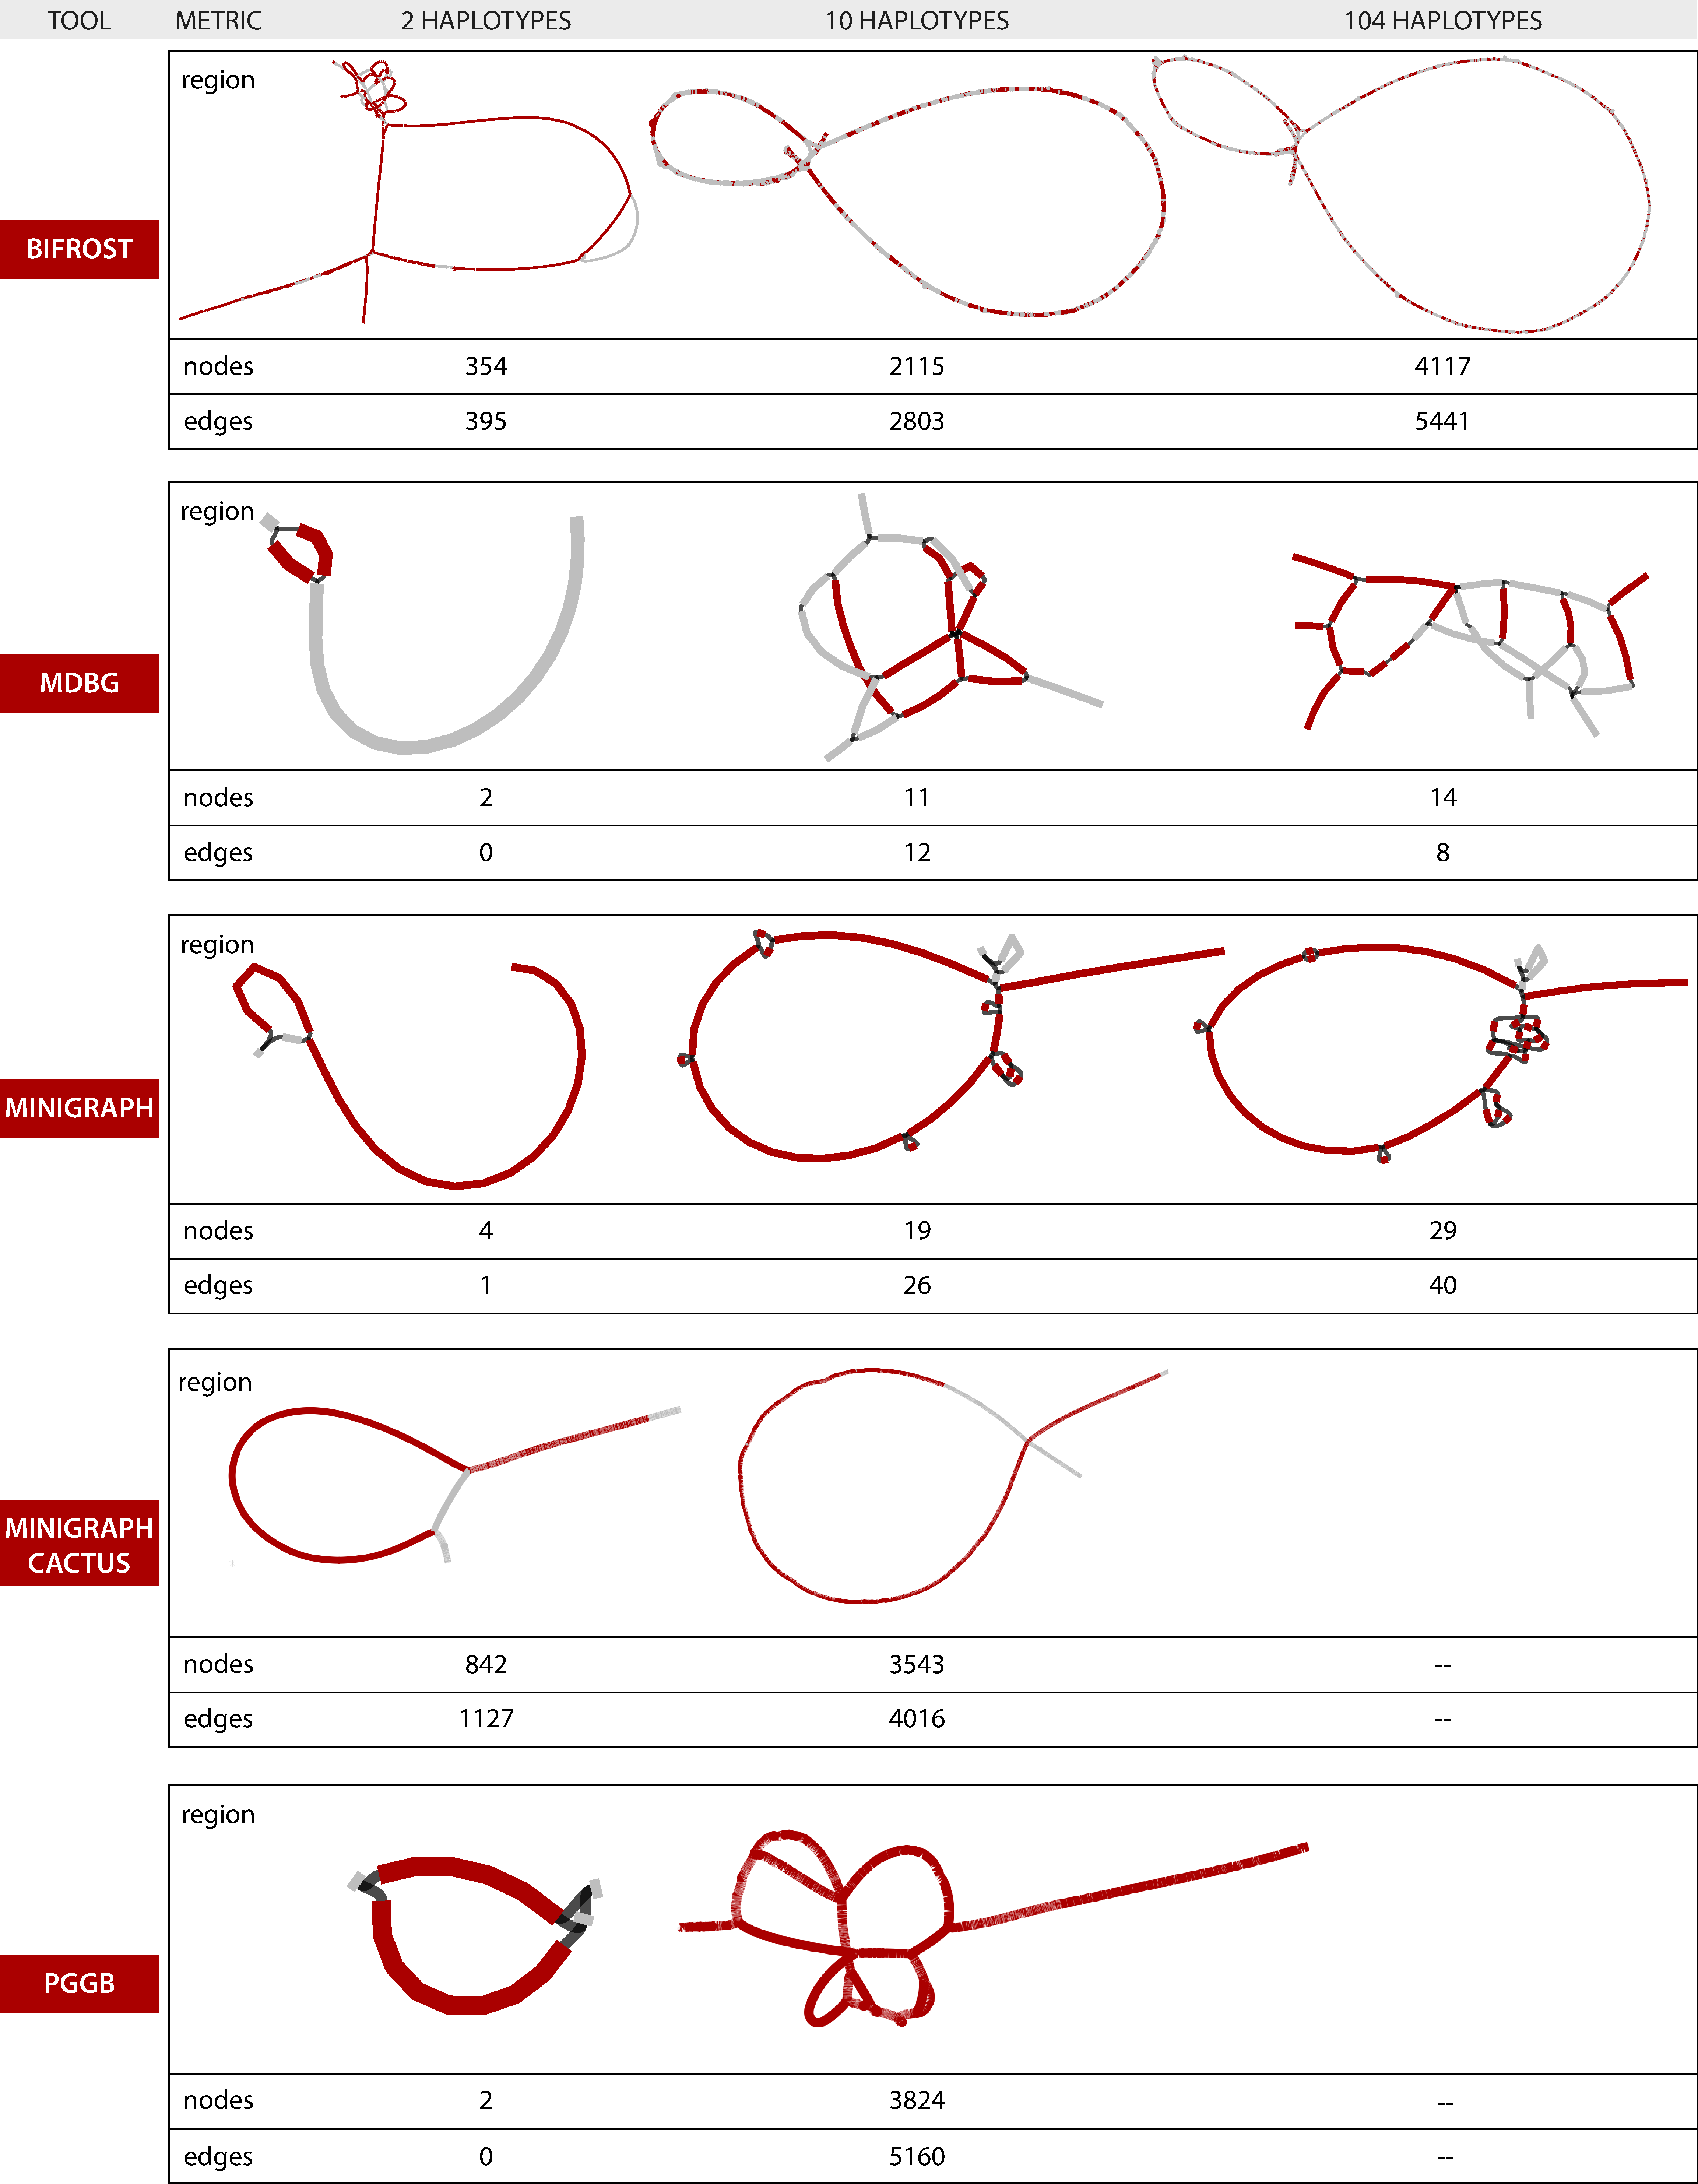
\includegraphics[width=0.95\textwidth]{figures/paperI/hla-a_corrected.pdf}
    \caption{Representations of the complex HLA region by five graph construction methods over three increasing large human pangenomes. 
 See caption of Fig.~\ref{fig:HLA-E} for details. 
 %.Nodes highlighted in red are the ones that contain part of the locus sequence. The number of nodes and edges displayed represent the ones directly or indirectly attributed to the sequences that represent the locus.
    }
    \label{fig:HLA-A}
\end{figure}

\subsection*{\textbf{Uncovering characteristics of graphical pangenome tools}}
\label{sec:uncovering}
The data structures generated by pangenome building tools are expected to facilitate comparisons between the input genomes. In addition pangenome graphs should be stored in such a way to be easily used by downstream applications.
We identify 8 important features for pangenome graph construction tools: i) stability, ii) editability, iii) accessibility by downstream applications, iv) haplotype compression performance v) ease of visualization, vi) quality of metadata and annotation. Two other but important features, scalability and interpretability of produced graphs, were already discussed in Sections "Scalability and characteristics of pangenome graph construction tools" and "Interpretation of variation in pangenome graphs: focus on two HLA loci". %\ref{sec:scalablility} and \ref{sec:loci}. 
Table \ref{tab:tools_consideration} summarizes some of the following considerations on the relative strength of the tools.

\paragraph{\textbf{\textup{Editability and dynamic updates}}}
%\noindent\textbf{EDITABILITY AND DYNAMIC UPDATES} 
As more high quality assemblies will be generated in the near future, haplotypes may be added to a pangenome, or replaced by improved versions. Updating an existing data structure instead of rebuilding it from scratch is both computationally and energetically efficient. 
However, many succinct data structures currently used in pangenome representation are static, i.e. cannot be updated. %Current
Some methods allow a restricted set of editing operations.
\minigraph allows to add new haplotypes on top of an already built graph. \bifrost provides C++ APIs to add or remove \mbox{(sub-)sequences}, \kmers and colors from the ccdBG.
\pggb, using \odgi~\cite{odgi}, allows specific operations that delete and modify nodes and edges and add and modify paths through the graph. As \mcactus can be opened with \odgi, it supports the same operations as \pggb. 
The current \mdbg implementation uses a dynamic hash table, but does not expose an interface that supports updates.

\paragraph{\textbf{\textup{Stability}}}
%\noindent\textbf{STABILITY} 
Counter-intuitively, a pangenome graph construction tool may in some cases generate different outputs when executed multiple times with the same haplotypes as input. This \emph{unstability} could be due to a permutation in the order of the sequences given as input, or non-determinism in the construction algorithm.
Yet in order to facilitate the reproducibility of results, pangenome building tools should generate an unchanged output from the same set of input sequences, independently of the particular run or the order in which these are given.
We performed two tests to evaluate tool stability: i) we run the tools 3 times using as input the same H10 dataset and ii) we run the tools twice on shuffled input sequences, i.e. changing the order of the haplotypes of H10. 

\bifrost and \mdbg constructed exactly the same pangenome on every test, as by definition, de Bruijn graphs are stable.
\minigraph generates identical graphs on identical inputs, but generates slightly different graphs when the input is permuted. Indeed the construction algorithm of \minigraph is order-sensitive as it augments the existing graph structure by aligning the next given haplotype to it and adding divergent sequences. 
\mcactus generates slightly different graphs on identical input. 
\pggb\ generated slightly different graphs while maintaining the same haplotype sequences in the paths. The overall representation of the input genomes is therefore preserved, while the topology of the variation graph varies. The first two of the three phases of the \pggb pipeline (all-vs-all alignment and graph imputation) produce the same result on different runs with the same input but differences arise when the order of the input haplotypes changes. Most of the differences in the graph topology are thus due to the final smoothing steps.

\paragraph{\textbf{\textup{Accessibility by downstream applications}}}
% \noindent\textbf{ACCESSIBILITY BY DOWNSTREAM APPLICATION} 
\label{subs:downstream}
To facililate their adoption, pangenome representations should be easily processed by downstream analyses. 
De Bruijn graphs are challenging to analyze due to their high number of nodes, edges, and redundancy (the $k-1$-overlaps between nodes).
Though De Bruijn graph representations usually support queries of presence/absence on nodes (as in \bifrost), they lack tools able to perform more elaborate analyses such as those discussed in Section "Interpretation of variation in pangenome graphs: focus on two HLA loci", e.g. incorporating haplotype information at the \kmer level. 
On the other hand, variations graphs with paths provide more flexibility, i.e. as in \pggb and \mcactus with the \odgi visualization toolkit.
Finally in \minigraph, which considers a narrower spectrum of variants, the absence of path information prevents haplotype-level analysis; haplotypes would need to be manually mapped back to the graph. 
The choice of the pangenome building tool depends on the envisioned application. \mbox{\pggb} and \mbox{\mcactus} graphs have been shown to outperform linear references for short read mapping, genotyping and RNA sequencing mapping \mbox{\cite{hdpr}}. As these two methods  are complex pipelines based on multiple tools where parameters have been carefully set, they can be more challenging to install and run than single integrated tools. \mbox{\minigraph} alone can also be used if the focus is on structural variation instead of SNPs or small indels, and to quickly produce a pangenome graph for complex loci visualization and interpretation. The dBG-based approaches show that, for example with \mbox{\bifrost}, they retain the same base-level information as more computational-heavy variation graph approaches, but the lack of tools to use them for analysis limits their adoption.

\paragraph{\textbf{\textup{Haplotype compression}}}
%\noindent\textbf{HAPLOTYPE COMPRESSION} 
Building a graph pangenome can be seen also as a way to store, compact and retrieve the input haplotypes. As the number of new assemblies is growing faster than the data storing capacity, pangenomes can potentially help save storage space. This is highlighted by the disk space reported in Table~\ref{tab:computational_metrics}, which is consistently smaller than the sum of haplotype sizes for all methods and datasets.

In order to losslessly retrieve the input genomes from a pangenome, the  representation has to store all variations from the original haplotype sequences as paths in the graph. \pggb and \mcactus fall into this category while the other three considered tools do not store paths, or do not consider all variations, thus they are lossy.

Of note, the GBZ tool~\cite{gbz} enables graph pangenomes that store paths in the GFA file format %(the consensus file format used) 
to be stored in a lossless compressed form. It uses a Graph Burrows-Wheeler transformation to compress the graph in a more efficient way than using gzip~\cite{gbz}. Using GBZ, the pangenomes generated by \pggb and \mcactus are losslessly compressed with space gains of 3.5-5x.


\paragraph{\textbf{\textup{Ease of Visualization}}}
%\noindent\textbf{EASE OF VISUALIZATION} 
Visualizing large graphs which exceed hundreds of thousands of node is a challenge that exceeds the scope of pangenomics. The H104 pangenomes  are difficult to visualize.
Among the visualization tools considered by the Human Pangenome Reference consortium~\cite{hpp}, 
only \bandage is able to display the \minigraph or \mdbg H104 graphs, which contains a few million nodes. We reduced the number of nodes and edges of \pggb, \mcactus and \bifrost H10 graphs by collapsing isolated subgraphs representing SNPs or indels up to 10k bp (using the command \texttt{gfatools asm -b 10000 -u}). % to be able to display them. 
%Generally, general-purpose graph drawing tools able to visualize graphs with millions of nodes are needed, in particular to extract and display specific loci.

\paragraph{\textbf{\textup{Quality of Metadata and Annotation}}}
%\noindent\textbf{QUALITY OF METADATA AND ANNOTATION} 
Augmenting pangenome structures with information from other omics data would increase pangenome relevance in biological discoveries. As biobanks are rapidly growing, more data is available on regulatory regions, transcriptomics, CNVs and other medically relevant traits~\cite{100000genomes,ucla}. Pangenome data structures could leverage such information, and some of the considered tools offer basic functionality in this sense.
\bifrost provides a function to link data to graph vertices through C++ APIs. \pggb and \mcactus, using \odgi, offer annotation capabilities through insertion of paths or BED records. \minigraph and \mdbg do not offer any annotation feature. 
Specifically, in order to enhance a pangenome graph with metadata (for example with genes and regulatory regions known variants), it is desirable to maintain compatibility with methods and data formats that use a linear reference. One could conceivably project data from a graph to a reference genome to continue downstream analyses using linear coordinates. A simple method to achieve this compatibility, in our view, is to store the reference genome of interest inside the graph pangenome that supports retrieving such a reference. Variation graphs built using \mbox{\pggb or \mcactus}, due to their locally acyclical and directed construction and their use of haplotype paths, store all the coordinates needed for such a task. Haplotype paths play an important role as they avoid additional mapping to the graph, by using the \mbox{\odgi}tool to extract or inject the required information. \mbox{\minigraph} does not store haplotype paths and requires mapping sequences to the graph to restore haplotype information. On the other hand, De Bruijn graphs, using associated color data, can record the membership of k-mers to a reference sequence, yet one cannot fully reconstruct a haplotype unless k-mers positions are also stored.
\begin{table}
\centering
 \caption{\textbf{Relative strengths of five pangenome graph construction tools}\\
 Explanation of rows:
 1) efficacy of construction algorithm, measuring wall-clock time;
 2) degree to which variants (e.g. SNPs) are retained;
 3) ability of a tool to perform well on large datasets, both in comparison to other tools but also compared to smaller datasets;
 4) ability to modify the produced data structure to add or remove haplotypes; 
 5) property of producing the same result irrespective of perturbations, such as permutation of the input order, and repeating the same run;
 6) existence of tools (and operations) that can be applied to the resulting graphs; 
 7) whether input haplotypes information is retained by the tools, and if so, its space efficiency;
 8) whether the entire graph can be directly visualized and interpreted; 
 9) easiness of 'zooming in' a specific genomic region and interpret variants;
 10) summarizes the functionalities provided by the tools to annotate the pangenomes with genomic data;
 11) ability to share information between the graph and a linear reference.
}
\resizebox{\textwidth}{!}{
\begin{tabular}{|l c c c c c|} 
 \hline
 Metric & \bifrost & \pggb & \mcactus & \minigraph & \mdbg\\
 \hline
  1) Construction speed & $\bullet\bullet\circ$ & $\bullet\circ\circ$ & $\bullet\circ\circ$ &  $\bullet\bullet\circ$ & $\bullet\bullet\bullet$\\
 \hline
 2)  Variations & $\bullet\bullet\bullet$ & $\bullet\bullet\bullet$ & $\bullet\bullet\bullet$ & $\bullet\bullet\circ$ & $\bullet\bullet\circ$\\
 \hline
  3) Scalablilty & $\bullet\bullet\bullet$ & $\bullet\circ\circ$ & $\bullet\circ\circ$ & $\bullet\bullet\circ$ & $\bullet\bullet\bullet$\\
 \hline
  4) Editability & $\bullet\bullet\bullet$ & $\bullet\bullet\circ$ & $\bullet\circ\circ$ & $\bullet\bullet\circ$ & $\bullet\circ\circ$\\
 \hline
 5) Stability & $\bullet\bullet\bullet$ & $\bullet\circ\circ$ & $\bullet\circ\circ$ & $\bullet\bullet\circ$ & $\bullet\bullet\bullet$\\
 \hline
 6) Accessibility by downstream applications & $\bullet\circ\circ$ & $\bullet\bullet\bullet$ & $\bullet\bullet\bullet$ & $\bullet\bullet\circ$ & $\bullet\circ\circ$\\
\hline
 7) Haplotype compression performance & $\bullet\bullet\circ$ & $\bullet\bullet\bullet$ & $\bullet\bullet\bullet$ & $\bullet\circ\circ$ & $\bullet\circ\circ$\\
 \hline
8) Ease of visualization  & $\bullet\circ\circ$ & $\bullet\bullet\circ$ & $\bullet\bullet\circ$ & $\bullet\bullet\bullet$ & $\bullet\bullet\bullet$ \\
 \hline
 9) Loci visualization and interpretability   & $\bullet\circ\circ$ & $\bullet\bullet\circ$& $\bullet\bullet\bullet$ & $\bullet\bullet\circ$  & $\bullet\circ\circ$\\
 \hline
  10) Metadata and annotation   & $\bullet\bullet\circ$ & $\bullet\bullet\bullet$ & $\bullet\bullet\circ$ & $\bullet\circ\circ$  & $\bullet\circ\circ$\\
 \hline
11) Compatibility with a linear reference coordinates & $\bullet\circ\circ$ & $\bullet\bullet\bullet$ & $\bullet\bullet\bullet$ & $\bullet\bullet\circ$  & $\bullet\circ\circ$\\
 \hline
\end{tabular}}
    \label{tab:tools_consideration}
\end{table}

\section{Discussion}
Five state-of-the-art pangenome graphs construction tools were compared on the representation of up to 104 human haplotypes. The approaches significantly differ in terms of speed, graph size, and representation of variations. We find that it remains computationally prohibitive to generate human pangenome graphs for hundreds of haplotypes, especially while retaining all variations. Each approach has its own set of strengths, and ultimately the choice of the method depends on the downstream application. In addition, several takeaway points emerged from our analysis.

First, our focused analysis of HLA loci revealed that de Bruijn graphs and variation graphs represent genomic variations equally well as pangenomes.  This is of particular importance as also shown by the draft human pangenome references~\mbox{\cite{hdpr}}: pangenomes are pivotal to trace complex and clinically relevant loci. While de Bruijn graphs are faster to construct, more stable, and scale better in terms of input size, the resulting graphs are challenging to interpret downstream. Variations graphs on the other hand are more practical to analyze at the expense of a less efficient construction step. Their visualization are more straightforward to interpret, mostly due to not having cycles, and provide insights into loci differences. 

Second, we can highlight two categories of pangenomic methods that have distinct application domains. \pggb, \mcactus and \bifrost store all possible variations, and keep haplotype information as paths or colors. They provide a complete picture of the set of variations in the input genomes which makes them difficult to analyze. They can be used for a large variety of genomic analysis, as shown for \mbox{\pggb} and \mbox{\mcactus}~\mbox{\cite{hdpr}}. \minigraph and \mdbg generate 'sketched' pangenome graphs that consider only large variants, ignoring smaller differences, and are more efficient to construct and visualize. They can be used for large scale characterization of variation in population, as proven for bacteria \mbox{\cite{mdbg}}.

Third, every tool possesses an exclusive set of features.
\pggb facilitates downstream analyses using the companion tool \odgi. It allows to precisely extract and browse any locus of interest. It is the only tool that generates variation graphs without a reference. It also keeps a lossless representation of the input sequences.
\minigraph generates a pangenome graph based on a reference sequence taken as a backbone. Its shines in the representation of complex structural variations, but does not include small or inter-chromosomal variations.
The pipeline \mcactus, that uses the \cactus base aligner, can be used to add small level variations on top of the \minigraph graph and to keep a lossless representation of the input sequences.
\bifrost illustrates that classical de Bruijn graphs are scalable, stable, dynamic, and store all variations. However, extracting information from them remain a challenge.
Lastly, \mdbg\ is the fastest construction method which generates an approximate representation of differences between haplotypes. As discussed in Section "Accessibility by downstream applications", these features enable different genomic analyses and downstream applications.

\section{Conclusions}
In conclusion, our results highligh the strengths and weaknesses of current pagnenome construction tools for human applications, with specific focus on how do they represent specific loci of medical relevance. We also provide insights on the features they possess and point out their best application domains.
In our view, future directions for human pangenomes building tools should focus on tackling efficiency bottlenecks, aiming to represent hundreds to thousands of haplotypes. Representations should further be lossless and represent the input haplotypes as paths in the graph. 
Such features would unlock many other applications such as lossless compression of haplotypes and cancer copy number variant analysis. 
Finally, we recognize the need for more user-friendly tools that can be used by biologists and that can translate complicated questions into  graph queries. While \odgi begins to address these questions in variation graphs, other approaches have not yet provided user-friendly interfaces. A package similar to \odgi for de Bruijn graphs would help fully realize their potential.

\section{Methods}
\subsection*{\textbf{Datasets and haplotypes collection}}
\label{sec:datasets}
In order to evaluate the state of current human pangenome representations, we sought to build a human pangenome that contains all publicly available high-quality human haplotypes. We collected from two different sources 102 different haplotypes from the genome of 51 individuals, and also used the two reference genomes, GRCh38 from the Genome Reference Consortium (GRC) \cite{grc} and CHM13 v2.0 cell line of the T2T Consortium~\cite{t2t}.
Five haplotypes correspond to Google Brain Genomics DeepConsensus \cite{deepconsensus} assembly dataset: they are hifiasm assemblies of PacBio Hi-Fi reads corrected with DeepConsensus. The average of their N50 is 37,99 Mbp. 
The remaining haplotype assemblies as well as the T2T reference are from the Human Pangenome Reference Consortium (HPRC) year-1 freeze~\cite{hpp}, and GRCh38 is from the GRC. Their average N50 is 40.3 Mbp. Since HG002 is contained in the DeepConsensus data, the HPRC HG002 haplotypes were not used.
The origin and the sex of the individuals are diverse %to aim for a 
and provide a fair representation of the diversity in human population: out of 51 total individuals, 21 are males and 30 are females and they represent 14 different ethnic groups, from US to Africa and Asia. We did not perform any additional selection, regarding sex and ethnicity, on these public datasets as our main goal was to use as many genomes as possible. However, the HPRC stated that the genomes were selected to represent genetic diversity in humans~\mbox{\cite{hdpr}}.

To evaluate the scalability of pangenome construction tools, we created three datasets of increasing size: 1) 2 haplotypes from the same individual, HG006, 2) 10 haplotypes from 5 different individuals (HG002, HG003, HG004, HG006 and HG00735) and finally 3) all of the 104 haplotypes. To test whether the order of the input sequences matters, we considered various random orderings for the 10 haplotypes in Dataset 2. Since \minigraph needs a reference sequence as fist haplotype in order to correctly build the graph, we generated specific 2 and 10 haplotypes datasets with the first haplotype replaced by the reference genome CHM13. This was applied to the \mcactus pipeline as well as it uses \minigraph variation graphs.

 \begin{table}
  \centering
  \setlength{\tabcolsep}{5pt} 
  \caption {\textbf{Description of the three datasets generated to test the scalability of the tools}
 \\
 Data sources: 
   $^1$ Google Brain Genomics~\cite{google-assemblies}; $^2$ Human Pangenome Reference Consortium~\cite{HPRC-haplotypes}; $^3$ 1000 Genomes Project~\cite{HPRC-haplotypes}; $^4$ Telomere to Telomere Consortium~\cite{HPRC-haplotypes}.
   \label{tab:datasets}}
  \renewcommand{\arraystretch}{1.2}
\begin{tabular}{|c c c|}
  \hline
  \centering
   Haplotypes & Project & Bases \\
   \hline
    2 & Google$^1$ & 5.9 Gbp\\
   10 & Google, HPRC$^2$ & 30 Gbp \\
    104 & Google, HPRC, 1KG$^3$, T2T$^4$ & 313.6 Gbp \\
    \hline
  \end{tabular}
\end{table}
 
\subsection*{\textbf{Pangenome graph construction tools}}
\label{sec:tools}

We evaluated tools that generate graph pangenomes as variation graphs and colored compacted de Bruijn graphs. Variation graphs are generally locally acyclic while de Bruijn graphs have cycles. In variation graphs, nodes represent sequences and edges represent immediate sequence adjacency without overlap. Variation graphs are generally easier to visualize and to interpret while challenging to construct at scale and, apart from \pggb, require a reference genome. In de Bruijn graphs (\dbg), nodes are \kmers (string of length k) and edges are (k-1)-overlaps between nodes. In practice, \dbgs are represented in a compact way where all nodes along unbranching paths are compacted into \emph{unitigs}. The resulting graph is called compacted De Bruijn Graph, where nodes are unitigs and edges represent (k-1)-overlaps. 
As shown in Figure \ref{fig:figure1}, de Bruijn graphs %are easier to construct and are more standardized but 
result in large graphs that pose visualization and interpretation challenges, in particular as there is no alignment to a reference.

\begin{itemize}
\item
\bifrost constructs dynamic, coloured compacted de Bruijn Graphs (\emph{\ccdbg}). It first generates a standard \dbg using an efficient variant of Bloom Filters and then computes the compacted \dbg from it.
Colors, i.e. identifiers representing the sample origin of each k-mer are added by storing an array per \kmer. A human genome \ccdbg typically consists of a single large connected component, as common \kmers are shared between chromosomes. This pangenome representation contains all the variations present in input sequences.

\item
\mdbg builds a variant of de Bruijn graphs called a minimizer-space de Bruijn Graph (\mdbg), which is efficient to construct as it only considers a small fraction of the input nucleotides. Color information is currently not supported in the implementation. Similarly to Bifrost, a \mdbg also typically represents a human genome as a single large connected component, albeit with orders of magnitude less nodes. Minimizer-space de Bruijn graphs mostly discard small variants, yet are sensitive to heterozygosity which creates branches in the graph.

\item
\minigraph constructs a directed, bidirected and acyclic variation graph iteratively by mapping new haplotypes using a combination of the minimap2 tool and the graph wavefront alignment algorithm. The first input sequence acts as a  backbone for the whole representation.
The sample(s) of each node are stored in a rGFA output file.
\minigraph considers only variations longer than 50 bps hence it is oblivious to isolated SNPs and small indels: even if it produces base-level alignment for contigs, the graphs are not a base-level resolution. The resulting graph is divided into connected components that correspond to the chromosomes present in the first given input genome.
%, yet can represent large divergent regions at base-pair resolution
\item
\mcactus is a variation graph construction pipeline that combines \minigraph to generate a structural variations graph and \cactus base aligner to generate base-level pangenome graphs of a set of input assemblies and embg: The definition of \label has changed! Check your packages! Replacing it with the kernel definition on input line 145.ed haplotypes paths. \cactus~\cite{cactus} is a highly accurate and scalable reference-free multiple whole-genome alignment tool, that in this pipeline considers the reference sequence used by \minigraph to ensure that the resulting variation graph is acyclic. The final graph is further normalized using GFAffix\cite{gfaffix}. The pipeline allows to generate multiple graphs, one for each chromosome, or produce a single graph that includes inter-chromosomal variants.

\item
\pggb is a directed acyclic variation graph construction pipeline rather than a single tool. It calls three different tools: pairwise base-level alignment  of haplotypes using wfmash \cite{wfmash}, graph construction from the alignments with seqwish \cite{seqwish}, graph sorting and normalization with smoothxg and GFAffix \cite{smoothxg,gfaffix}.
The resulting variation graph represents variations of all lengths present in the input sequences.
\end{itemize}


\begin{table}
\centering
\caption{ \textbf{URL, version, pangenome representation and parameters of the three analyzed tools.}\\ pggb/0.2.0 used wfmash v0.7.0, seqwish v0.7.3 and smoothxg v0.6.1.}
\resizebox{\textwidth}{!}{
\begin{tabular}{|c c c c c|} 
 \hline
Tool  &  Github repository & Graph type & Version & Parameters \\ 
 \hline \hline
\bifrost & pmelsted/Bifrost  & De Bruijn graph  & 1.0.5 & -k100 -c \\ 
 \hline
\pggb &   pangenome/pggb & variation graph  & 0.2.0 & -p 98 -s 10000 -k 311 -G 13033,13117\\ &&&& -O 0.03 -v -t 8 -T 8 -A -Z \\ 
\hline
 \minigraph & lh3/Minigraph  & variation graph &   0.18 & -cxggs\\ 
 \hline
  \mcactus & ComparativeGenomics  & variation graph &   2.2.3 & --maxLen 10000 --delFilter 10000000 \\ & Toolkit/cactus &&&\\ 
 \hline
 \mdbg  & ekimb/rust-mdbg  & De Bruijn graph &  1.0.1 & -k 10 -d 0.0001 --minabund 1 --reference\\ 
 \hline
\end{tabular}}
    \label{tab:url}
\end{table}



\section*{Supplementary Information}

\subsection*{\textbf{Benchmark infrastructure}}

Running time of pangenome construction tools was measured as wall clock time and peak memory as maximum resident set size using the \texttt{time} command. Other metrics were obtained with custom Python scripts. All benchmarks were performed on a Supermicro Superserver SYS-2049U-TR4, with 3 TB RAM and 4 Intel SKL 6132 14-cores @ 2.6 GHz, using 8 cores. \\

\subsection*{\textbf{TwoPaCo}}
\label{app:twopaco}
We did not consider \twopaco as it is redundant with \bifrost. Both methods construct the same de Bruijn graphs.
\twopaco is a method for constructing \ccdbgs by finding junction \kmers at the boundaries of unitigs or in branching nodes. It consists of two main steps in which it approximates the dBG with a Bloom filter in order to reduce the size of the problem and then runs a two pass highly parallel algorithm on it. It constructs ccdBGs similarly to \bifrost. \bifrost  is faster, supports edit operations, and accepts also reads other than assemblies as input. We tested both tools on NCBI datasets from three different known human variation regions part of the human leukocyte antigen (HLA) complex: HLA-A, MICB and TAP1. These loci have different number of sequences and have complexity and length. The resulting graphs have exactly the same k-mer content and substantially equal topology. The difference is that \twopaco considers sequences with IUPAC 'N' bases while \bifrost does not and that in some cases \twopaco renders some unitigs split in two or more consecutive nodes.

\subsection*{\textbf{Loci extraction method}}
\label{app:extraction}
For \bifrost and \mdbg graphs, nodes corresponding to the input sequences are identified with \graphaligner\cite{graphaligner} and the subgraph is extracted using the \bandage \emph{reduce} function. As the aligned nodes are not expected to represent the full diversity of the population in the pangenomes, the considered portion of the graph contains also nodes up to a certain distance from the aligned ones: 1 for \mdbg and 3 for \bifrost. This number is based on the size of the sequences spelled by the nodes and on the considered variations. Artifacts, mostly tips, that are not part of the locus of interest are removed with a custom python script. For \minigraph generated graphs, the \minigraph own alignment function has been used to identify the nodes and then \bandage is used to extract the subgraph. For \pggb, first we generate a bed file of the position of the region of interest in every haplotype used to construct the graph. The ranges are derived from aligning them to the locus sequence(s) using minimap2 \cite{minimap2}. The graph corresponding to the region is then extracted using the \odgi extract and \odgi view functions. For \mcactus we use the same strategy as \pggb, with the difference that the bed file is only for the reference CHM13, present in the graph. \\
The annotation of the specific loci in the subgraph is done using nodes from the alignment with \minigraph or \graphaligner to the subgraph. This makes it possible to highlight multiple sections in the region, as, for example, genes and pseudogenes of interest. 

\section*{\textbf{Availability of data and materials}} %Reproducibility and Data Availability
The scripts used to generate and analyse the pangenomes can be found at \cite{source-code-github}\cite{source-code-zenodo} under MIT license.
Google Brain Genomic assemblies can be found at \cite{google-assemblies}. \\
HPRC assemblies, CHM13 and GRCh38 can be found at \cite{HPRC-haplotypes}.

\section*{\textbf{Funding}}
R.C was supported by ANR Full-RNA, SeqDigger, Inception and PRAIRIE grants (ANR-22-CE45-0007, ANR-19-CE45-0008, PIA/ANR16-CONV-0005, ANR-19-P3IA-0001). This project has received funding from the European Union’s Horizon 2020 research and innovation programme under the Marie Skłodowska-Curie grants agreements No. 872539 and 956229.

\section*{\textbf{Author's contributions}}
FA, YD and RC conceived and designed the project. FA implemented the scripts. FA and PL ran the experiments. FA, YD, PL and RC wrote the paper. The authors read and approved the final manuscript.

%% Format bibliography like a section, not a chapter:
% \printbibliography[heading = subbibliography]
% \stopcontents[chapters]© Francesco Andreace, 2024

Series of dissertations submitted to the
Insitut Pasteur Paris, Universite’ de Paris Cite, University of Oslo
No. 1234
ISSN 1234-5678
All rights reserved. No part of this publication may be
reproduced or transmitted, in any form or by any means, without permission

\paragraph{Authors' affiliations}
\begin{description}
    \item[Francesco Andreace]
    Institut Pasteur, Université Paris Cité, G5 Sequence Bioinformatics \\
    Sorbonne Université, Collège doctoral \\
    25-28 Rue du Dr Roux, 75015 Paris


    \item[Pierre Lechat]
    Bioinformatics and Biostatistics Hub, Institut Pasteur, Université de Paris Cité \\
    25-28 Rue du Dr Roux, 75015 Paris

    \item[Yoann Dufresne]
    Institut Pasteur, Université Paris Cité, G5 Sequence Bioinformatics \\
    Bioinformatics and Biostatistics Hub, Institut Pasteur, Université de Paris Cité \\
    25-28 Rue du Dr Roux, 75015 Paris

    \item[Rayan Chikhi]
    Institut Pasteur, Université Paris Cité, G5 Sequence Bioinformatics \\
    25-28 Rue du Dr Roux, 75015 Paris
\end{description}

\section{Perspectives}

\begin{itemize}
    \item In perspective the work of this article could have been extended to provide a pipeline (on nextflow for example) to benchmark all pangnomes constructed independently of the data structure used to provide the features described on the paper. This would have provided a platform to independently benchmark new pangenomes and rendered the paper not only useful as review and hints for end-users but also as benchmarking for new methods or methods improvement;
    \item Among the features I could have included it would have been useful: \begin{enumerate}
        \item count SNPs (trivial for VGs, not trivial for DBGs);
        \item node length distribution;
        \item node degree distribution;
        \item conversion of variation graphs to De Bruijn graphs (extendin nodes smaller than k) to validate if they contain the same information/ did not loose information - see \minigraph example;
    \end{enumerate}
\end{itemize}
    %\author
{
    Francesco Andreace
    \and
    Pierre Lechat
    \and
    Yoann Dufresne
    \and
    Rayan Chikhi
}
\title{Comparing methods for constructing and representing human pangenome graphs}
\metadata
{
    Published in \emph{Genome Biology},
    November~2023,
    volume~24,
    issue~1,
    article number 274.
    \doi{10.1186/s13059-023-03098-2}.
}
\maketitle
\label{pap:gb_pdf}

\section{Motivation}
This paper originates from an early discussion, after completing a torough review of the state-of-the-art of computational pangenomics. What tool should be used if we would like to build a human pangenome for a large cohort of eukaryotes, for example humans. The answer is more complex than a list of widely used tools. There are multiple ways of representing a group of genomes to be analyzed or used jointly. One that took traction in the last few years has been graphs. Graphs can represent the sequence information as labels of nodes and the difference between the genomes as different paths in the graph. Depending on the particular representation, edges can represent adjacencies, i.e the genome is spelled by a walk on nodes connected by an edge, or overlaps , i.e. the suffix of a node is the prefix of the next node connected by the graph. In this article, we surveyed the the methods and tools that build such graphs, then tested them on different datasets and finally analyzed their features. The result is a small guide on which are the best applications for each of these tools and which are the weaknesses they suffer from.


\includearticle{sections/pangenome_paper}

\section{Perspectives}
The work of this article has adressed several key issues in both 
\begin{itemize}
    \item how to evaluate if a pangenome graph construction method is generating a data structure that faithfully represent the underlying genetic information and variations;
    \item In which areas in each methodology that should focus in order to produce for the community a useful tool.
\end{itemize}    
On this realization, this work could be relatively easily extended to provide a pipeline (on Nextflow, for example) to benchmark all pangnomes constructed independently of the data structure used to provide the features described on the paper. This would provide a useful platform to independently benchmark new pangenomes and rendered the paper not only useful as review and hints for end-users but also as benchmarking for new methods or methods improvement.
Moreover, other useful features could be added, among which
\begin{enumerate}
    \item count SNPs (trivial for VGs, not trivial for DBGs);
    \item node length distribution;
    \item node degree distribution;
    \item conversion of variation graphs to De Bruijn graphs (extending nodes smaller than k) to validate if they contain the same information and did not loose some (this behaviour is expected by \minigraph, or \mcactus, for example).
\end{enumerate}
Finally, the paper has been well received by the community, mostly because more methods in pangenomics are being published and a critical survey of which representation is better   

    %\author
{
    Victor Levallois
    \and
    Francesco Andreace
    \and
    Bertrand Le Gal
    \and
    Yoann Dufresne
    \and
    Pierre Peterlongo
}
\title{The Backpack Quotient Filter: a dynamic and space-efficient data structure for querying $k$-mers with abundance}

\metadata
{   
    Presented at \emph{RecombSeq}
    April-2024,
    \doi{10.1101/2024.02.15.580441}.
    % Published in \emph{Genome Biology},
    % volume~24,
    % issue~1,
    % article number 274.
}
\maketitle
\label{pap:second}

\section{Motivation}
This work stems from the very need of storing very large sequencing information from complex biological samples (like metgenomes) with the goal of being able to access it in a fast and randomized way. Complex biological datasets
\begin{abstract}
Genomic data sequencing has become indispensable for elucidating the complexities of biological systems. As databases storing genomic information, such as the European Nucleotide Archive, continue to grow exponentially, efficient solutions for data manipulation are imperative. One fundamental operation that remains challenging is querying these databases to determine the presence or absence of specific sequences and their abundance within datasets.

This paper introduces a novel data structure indexing $k$-mers (substrings of length $k$), the Backpack Quotient Filter (BQF), which serves as an alternative to the Counting Quotient Filter (CQF). The BQF offers enhanced space efficiency compared to the CQF while retaining key properties, including abundance information and dynamicity, with a negligible false positive rate, below $10^{-5}\%$. The approach involves a redefinition of how abundance information is handled within the structure, alongside with an independent strategy for space efficiency. 

We show that the BQF uses 4x less space than the CQF on some of the most complex data to index: sea-water metagenomics sequences. Furthermore, we show that space efficiency increases as the amount of data to be indexed increases, which is in line with the original objective of scaling to ever-larger datasets.
    
    \textbf{Availability:} \url{https://github.com/vicLeva/bqf} 
\end{abstract}

\footnotetext
{%
    University of Oslo,
    Postboks 1337 Blindern, 0316 Oslo, Norway,
    \href{mailto:fauthor@uio.no}{fauthor@uio.no}
}

\section{Introduction}

Genomic data sequencing is a powerful tool for understanding the intricacies of biological systems. Sequencing produces plain text, organized as reads in files. Most of these files are gathered in public databases like the European Nucleotidic Archive (ENA)~\cite{burgin2023european} that weighs 54.5PB by early 2024. The size of the databases follows exponential growth, and thus we need appropriate solutions to manipulate the data it contains. One simple operation that we are not yet able to achieve (in reasonable time and resources) is to query the database and then, for each dataset, answer if a sequence is present or absent. Even better, answer for each dataset how many times a sequence is present: its abundance. To this end, we use indexing data structures that can handle another representation of the data, making it easier to query afterward. Some of the current indexing data structures use sets of $k$-mers (substrings of length $k$, $k$ usually in $[20;50]$) as the representation to query. In this way, the proportion of shared $k$-mers between a query sequence and a dataset can be determined. The main operation is thus to determine for each $k$-mer in which indexed dataset it occurs and with what abundance (how many times it occurs in a dataset).

Due to the scale of databases to index, state-of-the-art tools often sacrifice precision for the sake of performance. This can be done through pseudo-alignment as defined in~\cite{themisto_2023}, breaking down the queried sequences into $k$-mers and comparing them against $k$-mers of the datasets, often encoded as a colored de Bruijn graph, as in Bifrost~\cite{bifrost_2020} or GGCAT~\cite{ggcat_2023}. Here, the graph construction is the main limitation of the methods. Other tools allow false-positive results by using Approximate Membership Queries (AMQ) data structures to enhance space efficiency~\cite{bigsi_2019, cobs_2019, squeakr_2018, kmtricks_2022, metaprofi_2023,  pac_2023}. They all have trade-offs between the index size and the false positive rate. By taking advantage of DNA and $k$-mers properties (small alphabet, redundancy of consecutive $k$-mers), the use of a simple associative array with super-$k$-mers~\cite{superkmer_2013} whose minimisers~\cite{minimisers_2004} have been hashed with a minimal perfect hash function~\cite{pthash_2021} can create exact and space efficient indexes such as SSHash~\cite{sshash_2022, sshash_2023}. However, apart from being static, exactness requires a trade-off with construction and query times.


Data structures form the core of the tools mentioned above. The choice of the structure impacts the performance and the range of operations available to the user. To illustrate, a Bloom filter~\cite{bloom_filter_1970} can insert elements after it has been built in memory, while an XOR filter~\cite{xor_filter_2020, binary_fuse_filter_2022} has better space usage, but is static. A Quotient Filter~\cite{quotient_filter_2012} allows more dynamicity than a Bloom filter as it can enumerate inserted elements and thus relocate elements in a smaller or larger structure as needed. The Quotient Filter is the backbone of the Counting Quotient Filter (CQF)~\cite{counting_quotient_filter_2017}, which can retrieve not only the presence or absence of a $k$-mer, but also its abundance. However, this structure results in suboptimal index size.

In this paper, we propose a new genomic data indexing structure, an alternative to the CQF called the Backpack Quotient Filter (BQF). It is more space-efficient than the CQF while still offering the same properties (abundance, dynamicity), at the cost of a negligible false-positive rate. We propose a novel way to handle the abundance information. We let the user control the balance between the index size and the precision with which the index encodes the $k$-mer counts/abundances.. In addition, we use the Fimpera~\cite{fimpera_2023} scheme to reduce each element's space usage. The BQF supports a large range of operations : random lookup (abundance), insert, enumerate, resize and delete (under circumstances).
In total, our tests show that at the price of a false-positive rate below $10^{-5}$\%, the BQF can index billions of elements and their abundance, using between 13 and 26 bits per element. Compared to existing solutions, the BQF has the fastest average query time, while being fully dynamic. It is, to our knowledge, the only data structure that cumulates these features.

\section{Material and Methods}

\subsection{Preliminaries}

\subsubsection{$k$-mers, pseudo-alignment, and indexing}

A $k$-mer is any sequence of given size $k$. It can be of any character but in our context a $k$-mer is a substring of a genomic sequence, \textit{i.e.} made up of nucleotides (A,C,G,T). The number of $k$-mers existing in two sequences provides a metric to measure the similarity between them, leading to the so called pseudo-alignment~\cite{themisto_2023}. In order to efficiently perform pseudo-alignments between any queried sequence and a dataset, we index its $k$-mers. Doing so, it is possible to know whether a $k$-mer belongs to the dataset or not.
Then, when querying a sequence $S$, all of its $k$-mers are individually queried in the index, enabling to compute the pseudo-alignment between $S$ and each dataset of a collection.

\subsubsection{Hash function}

A hash function is a mathematical transformation that takes an input (here a sequence of characters) and produces a number, called a hash value. In the current framework, the used hash function produces a value that is coded with a fixed-size number of bits. This transformation is designed to be deterministic, to produce an uniform distribution, and we want it to be as fast as possible. 

Given a hash function, two distinct elements are said in ``collision'' if they have the same hash value.
In this paper, we made the choice to use a xorshift~\cite{xorshift_2003} hash function, producing numbers between 0 and $2^{2k}$ for every $k$-mer. We use this~\cite{xorshift_64} xorshift hash function as it is a injective, preventing collisions.

Also, as long as we project the $k$-mers into values of $2k$ bits, the function is reversible. It means that we can retrieve the original $k$-mer from its hashed value.
The use of a non injective hash function would also be possible but would imply the impossibility to enumerates the elements entered in the data structure. This would prevent, for example, the resizing of the data structure. As we want a fully dynamic data structure, we made the choice of using the injection.%it is not implemented in the BQF repository.

Finally, we need a hash function to randomize the positions of elements in the structure and thus avoid the creation of long runs of elements that would slow down insertions and queries.



\subsection{Quotient Filter (QF)}
The work we present, called the Backpack Quotient Filter (BQF), is based on the Quotient Filter (QF) structure~\cite{quotient_filter_2012}. In this section, we provide a brief overview of the fundamental aspects of the QF structure, which is essential for comprehending our contribution. We give a more detailed description in the Supplementary material.

A QF is a data structure that is used to store a set of elements.
It is composed of a table with $2^q$ slots, each of fixed size $r$, where $q$ and $r$ are initially defined by the user. $q$ and $r$ are subject to change as the size of the table may change.
It utilizes a hash function $h$ that hashes elements to integers of $q+r$ bits.
When an element $x$ is inserted, its hash value $h(x)$ is computed and split into two parts: 
\begin{itemize}
    \item $h_0(x)$ of size $q$ bits, called the ``quotient''. It is used as an address in the table;
  \item $h_1(x)$ of size $r$ bits, called the ``remainder''. It is a fingerprint and is effectively stored in memory. $h_1(x)$ is inserted at the address $h_0(x)$.
\end{itemize}

To query the presence of an element $y$ in the structure, $h_0(y)$ and $h_1(y)$ are computed. Finding $h_1(y)$ at position $h_0(y)$ implies that $y$ is, with known probability, present.
Figure~\ref{fig:BQF} pictures the insertion step at slot 3, where solid hatched green lines symbolize the $r$ bits of the remainder, inserted at address 3.

\begin{figure}[ht]
   \includegraphics[width=\textwidth]{figures/paperII/example.png}
   \caption{A 32 slots long BQF ($q$=5). First line represents the metadata bits (see~\cite{counting_quotient_filter_2017} for more details). This short example does not represent blocks (\textit{cf.} supplementary data) in the BQF for simplicity. Each slot has a size of $r$ bits for the remainder with $c$ bits for counts and 2 bits of metadata: $occupied$ and $runend$. A circled address $Q$ means that at least one element $x$ such that $h_0(x) = Q$ has been inserted. Multiple remainders sharing the same color in the BQF have been originally inserted at the same address and form a run (\textit{cf.} supplementary data). Empty metadata bits are set to 0.}
   \label{fig:BQF}
\end{figure}

Originally the QF is said to be a probabilistic data structure: with a non-zero false-positive rate when querying elements. In the current framework, as we use an injective hash function, the false-positive rate is zero. However, as explained later (Section \ref{ssec:fimpera}), we use an additional technique that does not exactly query the actual stored elements, and that generates a negligible but non-zero false positive rate at query time.

In practice, the metadata bits used, the probing method and the global organization of the QF we use is based on the Rank \& Select Quotient Filter first proposed in~\cite{counting_quotient_filter_2017}. We detail this structure and the implementation in the Supplementary Materials.


\subsubsection{Abundance in Quotient Filters} 

As previously defined, the Quotient Filter structure is enough to handle the presence or absence of $k$-mers. It is possible to adapt the structure so it can store each $k$-mer alongside with its abundance in the indexed dataset. The Counting Quotient Filter~\cite{counting_quotient_filter_2017} (CQF) is an example of a QF with abundance. 

In the CQF, the abundance of each inserted element can be stored using the following process. A slot is used to store a remainder or an abundance value. If an element $x$ has its abundance $1 \leq n \leq 2$, then the element is inserted $n$ times (with $n=2$, two consecutive slots store $h_1(x)$). When $n > 2$, $h_1(x)$ is stored twice and these two slots act like boundaries in the table, defining the beginning and the end of the counter. Then $n-2$ is encoded and stored between both boundaries, using potentially two slots or more. An extra slot holding a $0$ might be necessary to maintain consistency in the runs. The point here is that this approach uses 2 slots when $n = 2$ and 3 or more when $n > 2$.

In the following section, we present our contribution, called the Backpack Quotient Filter, improving both the way the counts are stored and highly optimizing the size taken by each element to be queried.

\subsection{The Backpack Quotient Filter}\label{ssec:mm:bqf}

\subsubsection{Storing the abundance}
In the BQF, the abundance of each element is stored using the following approach. 
As represented in Figure~\ref{fig:BQF} each slot stores both a remainder and an abundance value. More precisely, each slot stores $r$ bits for the remainder, and $c$ extra bits are used to encode the abundance value. 
The $c$ parameter is a user-defined parameter. The choice of $c$ has a direct impact on the BQF size, adding $c\times 2^q$ bits. The maximum value for abundance is $2^c$ and the value can be an exact count, or an order of magnitude (e.g. encoding of $log_2$ values), offering flexibility based on precision requirements.

If the value of a count overflows the number of bits allocated, the $2^c$ value is stored and the answer at query time is $\ge 2^c$.

Compared to the CQF, the BQF uses only one slot per element, regardless of the abundance of this element, but at the same time it uses more bits per slot. However, thanks to the proposition described in the next section, we can reduce the size of the stored remainder. In this way, we cancel out this effect, even using less space per element while storing abundances.

On a side note, the name Backpack Quotient Filter comes from the fact that every slot handles its own counter, as if it was carrying a backpack.

\subsubsection{Reducing the space usage} \label{ssec:fimpera}

In order to reduce the space usage, we take advantage of a method called Fimpera~\cite{fimpera_2023}. This method is originally
designed to reduce the false-positives of data-structures having non-zero false positive rates. 

Focusing on the presence/absence only, the key idea can be summarized as follows: if a word is present in a text, then all of its sub-words are present. Conversely, if any sub-word is absent, then the whole word is absent. In practice, instead of indexing the $k$-mers from a dataset, we insert all its $s$-mers, with $s\leq k$. At query time a $k$-mer is considered as indexed if and only if all its $s$-mers are indexed in the structure. In the general case of querying a $k$-mer in an structure with collisions, this approach enables to lower the false positive rate of the query because all $s$-mers of a specific $k$-mer need to be false positives to create a false positive $k$-mer. 

The same idea can be exploited when taking the abundance into account. The abundance of a $k$-mer is at most equal to the least abundant $s$-mer it is composed of. Therefore, we store the abundance of s-mers in the filter and report the abundance of a queried k-mer as the minimum of the abundances of the s-mers composing it. The techniques described in~\cite{fimpera_2023} explain how this approach does not have a negative impact on query time and may even improve it.
When applied to a structure having collisions, this approach limits the overestimation of the abundance, as all the $s$-mers of a queried $k$-mer have to be overestimated to overestimate the real abundance of this $k$-mer. 

In the BQF, we do not have any collision. We apply this approach to gain space instead.

Let us first study the size of the reversible hash value, used to store words on a four-character alphabet. Each character (here $\{A,C,G,T\}$) requires two bits for its encoding. Hence, encoding a word of length $\ell$ requires $2\ell$ bits. As we use a reversible hash function, the size of the hash value requires the same size as the original encoded data, $2\ell$. 

By inserting $s$-mers, smaller than $k$-mers, the size of the reversible hash value of each inserted element becomes $2s$ instead of $2k$. If we denote by $z$ the difference between $k$ and $s$, the gain is $2z$ bits per element. In the BQF structure, the consequence is that the size of each slot is decreased by $2z$. All in all, applying this approach enables to save $2^q \times 2z$ bits. The same hash function is used, with the same  properties of injection and reversibility of stored elements.

A drawback of using this approach is the loss of the enumerating feature for $k$-mers. The hash function is still reversible but because we have $s$-mers in the filter, we can only reconstruct (and thus enumerate) these $s$-mers and not the $k$-mers we want to query. It is important to note that we only lose the $k$-mers enumeration, not the dynamicity: resizing the BQF remains possible.

If the counters are not exact, \textit{i.e.} if orders of magnitude are indexed then inserting and deleting new elements is no longer a trivial task. We will study the possibilities of updating the BQF in this case in future work.

The second drawback of applying this approach is the creation of a new kind of false positives, called ``construction false positives''. 
The existence of construction false positive is explained by a simple sentence: a $k$-mer may be absent but all of its $s$-mers may be present. We meet this case if each $s$-mer of an absent $k$-mer $x$ has been individually inserted through the present $k$-mers sharing $s$-mers with $x$. 
Overestimations can also happen, a study of this probability has been realised in fimpera paper~\cite{fimpera_2023}.






\subsubsection{Theoretical influence of the $s$ parameter}\label{ssec:s_influence}
We now detail the theoretical consequences of reducing the size $s$ of indexed elements, with $s \in ]0, k]$. 
\begin{enumerate}
    \item Decreasing $s$ increases the ``construction false positive'' rate.
    The smaller the $s$ value is, the higher is the probability that a queried $k$-mer, non existing in the indexed set, has all its $s$-mers existing in this set. 
    \item Decreasing $s$ may increase the number of indexed $s$-mers in short reads datasets. A sequence of size $\ell$ contains ($\ell-k+1$) $k$-mers and ($\ell-s+1$) $s$-mers. Hence, it contains $z=k-s$ additional $s$-mers than $k$-mers. This is negligible while indexing for instance an assembled genome.
    But when it comes to index millions of reads with low redundancy between them, as this is the case in our experimentations using sea-water metagenomes, each of the million reads contains $z$ more $s$-mers than $k$-mers, with a low redundancy between reads.
    \item Decreasing $s$ decreases the size taken by each indexed $s$-mer, which is the expected effect. This is the main advantage of the approach. Recall that the total size of structure is reduced by $2^q \times 2z$ when using $s$-mers instead of $k$-mers. Hence the smaller $s$ is, the more space is saved.
\end{enumerate}

In general, the results presented Section~\ref{ssec:s_impact} suggest that the size of the data structure decreases as $s$ decreases, despite the conflicting effects of the last two previous points. Selecting small $s$ values only has the potential to increase the construction false positive rate. However, when using recommended values, it stays below $10^{-5}\%$. 

\subsubsection{Doubling the number of slots when the structure is full}\label{sssec:full}
One of the main advantage of building the QF with an injective hash function is that conversely to a Bloom filter for instance, when the structure is full, it is possible to double its number of slots (from $q$ to $q+1$).
During this process, the hash value of each element remains the same, but the way it is distributed between the quotient and remainder changes. This occurs because, after doubling, $q+1$ bits are used to represent the address, while $r-1$ bits are used for the remainder.
Finally, the total number of stored elements faces no theoretical limitation.

In practice, for performances reasons, one doubles the number of slots when the ``load factor'' (number of stored elements divided by the number of slots) becomes bigger than 95\%. Load factor effect experiments have been performed here~\cite{counting_quotient_filter_2017}.


\subsubsection{Number of bits per stored element}\label{sssec:bit_per_element}
As stated, the basis of the QF data structure is to use the address of stored elements as a part of their hash value. As a consequence, the size of the remainder stored for each element decreases when the number of slots increases. This is not linear.  Let us consider the initial scenario, where the QF is composed of $2^q$ slots in which $r$ bits per slot are used as remainder. In this case, the BQF uses $2^q\times(r+c+3)$ bits, as for each stored element, $r$ bits store the remainder, $c$ bits are used to store the abundance, and 3 additional metadata bits are used by the structure itself ($runend$, $occupied$ and a third one, $offset$, explained in supplementary data).

Now consider that the size of the structure doubles in order to index more elements. The structure then contains $2^{q+1}$ slots. In this situation, $q+1$ bits indicate the address of each slot,  and so the remainder of each element decreases to $r-1$ bits instead of $r$. In this case, the total size of the structure becomes $2^{q+1}\times(r-1+c+3) = 2^{q+1}\times(r+c+2)$. As the structure grows, $q+r$ stays constant and the slots become smaller.

Note that this practical effect ends when the remainder is empty, in which case the full hash value of each element is entirely given by the address of the element. This presents a theoretical perspective. In the case of $k$-mer indexing, where conventional $k$ values are typically around 30, approximately 140 petabytes would be needed to contain the $4^k$ slots (representing the number of possible distinct $k$-mers).

\section{Results}
We present experimental results on real metagenomic datasets. The objective is to compare the performances obtained with the BQF with those obtained using state-of-the-art data structures for indexing $k$-mers together with their abundances, based on the Quotient Filter: the CQF~\cite{counting_quotient_filter_2017} and on the counting Bloom Filter: the CBF~\cite{fimpera_2023}. We also included a comparison with Bifrost~\cite{bifrost_2020} and SSHash~\cite{sshash_2023}. Both of these approaches allow for querying indexed $k$-mers, but they have significant differences in their main features, which are summarized below.

These results also enable to show the impact of the unique parameter introduced by BQF: the $s$ value. We also show the influence of the number of indexed elements on the whole data structure size.


The version used for BQF is v1.0.0. Details about protocols and links to datasets are available online~\cite{protocols}.

\subsection{Used datasets} \label{ssec:setup}

Our results were obtained on three distinct metagenomic datasets in which we exclusively considered $k$-mers present two or more times. 

\begin{itemize}
    \item Dataset ``\textit{sea-water34M}'': 34 million Illumina reads from the \textit{Tara} Oceans sequencing project. The uncompressed \textit{fastq} file is  7.7GB. It contains 257M distinct 32-mers and 346M distinct 19-mers occurring at least twice.
    \item Dataset ``\textit{sea-water143M}'': 143 million Illumina reads from the \textit{Tara} Oceans sequencing project. The uncompressed \textit{fastq} file is  33GB. It contains 1.2B distinct 32-mers and 1.5B distinct 19-mers occurring at least twice.
    \item Dataset ``\textit{gut}'': 13 million reads from pig microbiota Pacbio sequencing. The uncompressed \textit{fastq} file is 42GB.  It contains 475M distinct 32-mers and 420M distinct 19-mers occurring at least twice.
\end{itemize}  

These sea-water and gut microbiota metagenomic datasets are representative of a highly complex environment, with a large diversity content. For instance, there are 9.5 billion $k$-mers in \textit{sea-water143M} dataset, leading to a set of 5.7 billion distinct $k$-mers. Among them, only 1.2 billion are present twice or more. For the \textit{gut} dataset, we counted 22 billion $k$-mers, 1.2 billion distinct ones and 0.475 billion are present twice or more. We present in Supplementary Materials a visualisation of the $k$-mer spectrum of the sets \textit{sea-water143M} and \textit{gut}. They illustrate the complexity of these datasets, where there is no peak linked to the specific presence of one or more species. %in A $k$-mer spectrum is available in supplementary materials for a whole visualization. 


\subsection{Compared performances}
In this section, we present a comparative analysis between BQF and CQF (\url{https://github.com/splatlab/cqf}, commit 68939f5). Both structures use the same Xorshift hash function, a PHF, ensuring no collisions. We also compare with results obtained with a counting Bloom filter (CBF), with one hash function, implementing the Fimpera approach (\url{https://github.com/lrobidou/fimpera}, commit 662328d). Both CBF and BQF use 5 bits for counters ($c = 5$), allowing a maximal abundance value of 64 as we store exact values. 
%The objective is to query 32-mers in these datasets, so we have $k=32$. 
BQF and CBF use the Fimpera approach, initialized with $k=32$ and $s=19$, thus 19-mers are counted and inserted. 
The sizes of the BQF and CQF are determined solely by the total number of elements plus the element abundances for the CQF. Regarding the CBF, we decided to create a CBF of the same size as the BQF. This ensures fair comparisons when considering a fixed amount of disk space.
The choice of parameters is discussed further in this section. 

We also show results obtained by Bifrost (version 1.3.1) and SSHash (version 3.0.0). Those comparisons are not exactly fair as these tools embed additional features (computing pre-assembly of the data in the so-called compacted de Bruijn graph, possibly indexing multiple datasets for Bifrost) while Bifrost cannot index the abundance, and while SSHash is a static data structure. However, it is interesting to present these results as they show that these state-of-the-art tools —which are not specifically designed for the task of only indexing $k$-mers with their abundances— are not optimal for this task.
%but they show the limitations of these existing state-of-the art tools in the simple context of indexing only $k$-mers with their abundances.

\subsubsection{Experimental setup}
We computed the build time and the query time for each approach. In addition to the building time, the results show the pre-processing time, \textit{i.e.} the time used to obtain the correct input file from the raw compressed \textit{fastq} file (counted $k$-mers for CQF, CBF and BQF, and SPSSs~\cite{RahmanMedvedevRECOMB20} for SSHash). 

The parameters are $k=32$ for CBF, CQF, and BQF, $c=5$ (counters size for BQF, CBF), and $s=19$ ($19$-mers were inserted for BQF, CBF). For SSHash and Bifrost, we used $k=31$ as using $k=32$ would have doubled the $k$-mer encoding size for Bifrost, and because SSHash uses $k\leq31$. 
%The parameters are $k=32$ for CBF, CQF, and BQF, $k=31$ for SSHash and Bifrost, $c=5$ (counters size for BQF, CBF), and $s=19$ ($19$-mers were inserted for BQF, CBF). 
Bifrost used 4 threads and $m=17$ for SSHash (minimisers size). 

Positive queries in a dataset $\mathcal{D}$ are $k$-mers reads from $\mathcal{D}$ itself. Negative queries are $k$-mers from randomly generated sequences (between 80 and 120 nucleotides). Around 2 billion $k$-mers over 30 million sequences were positively queried. Around 7 billion negative $k$-mers over 100 million sequences were negatively queried. 

BQF and CQF sizes are measured experimentally. Their size corresponds exactly to their theoretical value, also showing that, thanks to the simplicity of the structure, no space overhead is required. CBF size was chosen to be the same as BQF's. SSHash size is the one displayed by the tool at the end of the building step. Bifrost size is measured as the peak memory usage after loading the graph and the index in memory (from binary representation on disk). 

The executions were performed on the GenOuest platform on a node with $4 \times 8$ cores Xeon E5-2660 2,20 GHz with 128 GB of memory.
\subsubsection{Comparative results}
\begin{table}[ht]
\resizebox{\textwidth}{!}{
\begin{tabular}{rr|rrrr|rrr}
Dataset  & Structure & 
\begin{tabular}[c]{@{}r@{}}\textbf{Index size} \\ \textbf{on disk} \\ (GB)\end{tabular}     &   \begin{tabular}[c]{@{}r@{}}\textbf{Bits per }\\ \textbf{element}\end{tabular}   & 
\begin{tabular}[c]{@{}r@{}}Pre-processing +\\Build time (s)\end{tabular}                    &   \begin{tabular}[c]{@{}r@{}} Build \\ peak memory \\ usage (GB) \end{tabular}    & 
\begin{tabular}[c]{@{}r@{}}Pos. query \\ throughput \\ (kmer/s)\end{tabular}                &   \begin{tabular}[c]{@{}r@{}}Neg. query \\ throughput \\ (kmer/s)\end{tabular}    & 
\begin{tabular}[c]{@{}r@{}}FP rate \\ (\%)\end{tabular} \\
    & &      &    &         &         &         &       \\ \hline
    & &      &    &         &         &         &       \\
\textit{sea-water34M}       & Bifrost           & 5.84      & 177   & 1,041$^\alpha$         & 5.84  & 2,687,272     & 3,224,789     & 0     \\
                            & SSHash            & 0.40      & 12    & 1,165$^\beta$ + 67     & 2.46  & 1,150,224     & 1,354,394     &  0     \\ 
                            & {CQF}             & 4.58      & 139   & 215$^\gamma$ + 210     & 4.60  & 1,448,481     & 2,121,294     & 0     \\
                            & CBF               & 1.11      & 26    & 219$^\gamma$ + 429     & 1.11  & 205,306       & 285,061       & $4.8\times10^{-6}$      \\
                            & \textbf{BQF}      & 1.11      & 26    & 219$^\gamma$ + 257     & 1.11  & 2,052,016     & 2,934,776     & $1.6\times10^{-6}$      \\
    & &      &    &         &         &         &       \\ \hline
    & &      &    &         &         &         &       \\
\textit{sea-water143M}      & Bifrost       & 17.57     & 114    & 6,074$^\alpha$          &  21.94  & 1,321,360     & 2,581,435     & 0     \\
                            & SSHash        & 1.97      & 13    & 5,875$^\beta$ + 361      &  11.15  & 871,794       & 1,122,606     & 0      \\
                            & {CQF}         & 17.25     & 113   & 771$^\gamma$ + 949       &  17.52  & 1,097,099     & 1,602,930     & 0     \\
                            & CBF           & 3.93      & 21    & 780$^\gamma$ + 2,039     &  3.93   & 195,177       & 281,244       & $5.8\times10^{-5}$      \\
                            & \textbf{BQF}  & 3.93      & 21    & 780$^\gamma$ + 1,101     &  3.93   & 1,791,640     & 2,616,583     & $3.0\times10^{-5}$        \\
    & &      &    &         &         &         &       \\ \hline 
    & &      &    &         &         &         &       \\
\textit{gut}                & Bifrost           & 5.84      & 99    & 5,972$^\alpha$          &  5.84  & 8,448,220     & 3,114,457     & 0     \\
                            & SSHash            & 0.58      & 10    & 2,558$^\beta$ + 113     &  3.79  & 4,438,401     & 1,286,876     & 0      \\
                            & {CQF}             & 8.90      & 150   & 1,178$^\gamma$ + 396    &  9.01  & 1,598,278     & 1,948,436     & 0     \\
                            & CBF               & 1.11      & 21    & 1,085$^\gamma$ + 468    &  1.11  & 352,201       & 284,545       & $1.6\times10^{-6}$      \\
                            & \textbf{BQF}      & 1.11      & 21    & 1,085$^\gamma$ + 341    &  1.11  & 4,582,535     & 2,821,471     & 0     \\
    & &      &    &         &         &         &       \\ \hline
    \multicolumn{8}{l}{\footnotesize $^\alpha$ Bifrost does not require pre-processing step} \\ 
    \multicolumn{8}{l}{\footnotesize $^\beta$ BCALM~\cite{bcalm_2016} (https://github.com/GATB/bcalm, version 2.2.3) for unitigs + UST~\cite{RahmanMedvedevRECOMB20} (https://github.com/jermp/UST, commit b3d0710) for simplitigs} \\
    \multicolumn{8}{l}{\footnotesize $^\gamma$ KMC~\cite{kmc_2017} (https://github.com/refresh-bio/KMC, version 3.2.4) kmer counting}
\end{tabular} 
}
\caption{Comparative performances. Recall that Bifrost and SSHash do not index the same number of elements than CQF, CBF and BQF, explaining the difference in terms of number of bits per element as compared to the structure size. Given its computation time ($\geq 24$ hours on the \textit{sea-water143M} dataset), we report SSHash results only for the \textit{sea-water34M} dataset. }
\label{table:results}
\end{table}



\paragraph{Comparing CQF and BQF}
Compared to the CQF, the major advantage of the BQF is in terms of space. As shown Table~\ref{table:results}, the BQF is approximately four times smaller than the CQF for every indexed dataset. %at the price of very low false positive rates ($10^{-5}$ or $10^{-6}$\%). 
The same advantage is found in terms of space efficiency (bits/element), being approximately 5 to 7 times more efficient. However, one drawback is the occurrence of false positive calls, which are generally less than $10^{-5}\%$ and can even be as low as 0\% in the gut data set. 

\paragraph{Comparing CBF and BQF}
The results presented Table~\ref{table:results} indicate that the false-positive rate is slightly better with the BQF compared to CBF. However, both approaches still have a very low false positive rate of approximately $10^{-5}$\%, which is insignificant for indexing and pseudo-alignment applications. BQF offers several significant benefits over CBF. First, BQF allows for faster time queries, with an average speed improvement of 50 times compared to CBF. Additionally, BQF does not have any theoretical limitations on the number of stored elements, unlike CBF which is designed for a fixed maximum number of elements that cannot be updated. Finally, the elements stored in a BQF (the $s$-mers) can be enumerated, while this is not the case with the CBF.

\paragraph{Abundance overestimation due to the Fimpera approach}
In this work, we did not recompute the so-called overestimation inherent to the Fimpera abundance representation. This overestimation is in the order of 1\% to 2\% according to the results presented in~\cite{fimpera_2023}, meaning that $1$ to $2$\% of the abundances of true positive calls are overestimated. Furthermore, for those results that were overestimated, the average difference was shown to be approximately 1.07 times the correct abundance range. All in all, this slight overestimation, limited to less than 2\% of the calls, has no significant impact while estimating the abundance of a query composed of at least dozens or hundreds of $k$-mers.

\paragraph{Bifrost and SSHash results}
As shown by results presented Table~\ref{table:results}, Bifrost is approximately two times slower than BQF to build the data structure and more than twice as slow to perform negative queries. It uses approximately 4.5 times more space per element, and more importantly, it does not provide the abundance of $k$-mers. 
The SSHash approach, for its part, taking advantage of super-$k$-mers~\cite{superkmer_2013}, uses approximately 2 times less space per element than BQF. However, it is static and is nearly two orders of magnitude slower to construct, drastically limiting its application to large-scale projects.

\subsection{Impact of size of the indexed $s$-mers}\label{ssec:s_impact}
As stated earlier, the BQF structure stores $s$-mers, to emulate $k$-mers at query time, with $s\leq k$.
The choice of the $s$ value has several consequences that are described Section~\ref{ssec:s_influence}, and that we propose to empirically observe here.


\subsubsection{Effect of $s$ on the number of construction false positives}
\begin{figure}[ht]
    \centering
   \includegraphics[width=0.75\textwidth]{figures/paperII/fig_fimpera_publi.png}
   \caption{Empirical observation of the evolution of the construction false positive rate with respect to $s$. Indexed dataset: ``\textit{sea-water34M}'', querying random 32-mers. The value of $s$ is decreasing as it starts from $k$, then we increase the difference between $k$ and $s$.}
   \label{fig:fimpera:cfp}
\end{figure}

Figure~\ref{fig:fimpera:cfp} illustrates that using any value of $s$ bigger than 17 enables to limit drastically the construction false positive rate. 
When $s$-mers become smaller than 17 nucleotides, the probability they appear by chance in sequences composed of millions of characters on the $\{A,C,G,T\}$ alphabet becomes close to 1. In this case, mostly any $k$-mers can be constructed from these $s$-mers, explaining the nearly 100\% construction false positive rate.

Note that the shape of this curve is highly correlated with the probability that an element of size $s$ appears by chance in a sequence of size $\ell$. This probability is equal to $1-\left(1-\frac{1}{4^s}\right)^\ell$. In concrete terms, this allows a user to reliably determine a value of $s$ knowing $\ell$, even approximately. The value of $\ell$ can be approximated thanks to the number of distinct $k$-mers in the dataset (as this is the case in Figure~\ref{fig:fimpera:cfp}), efficiently computed by ntCard~\cite{Mohamadi2017ntCardAS} for instance.

These results assume a uniform $ATCG$ distribution, we plan for future work to study the impact of high or low $GC$ content.


\subsubsection{Effect of $s$ on the structure size}
Recall that decreasing $s$ has two opposite effects on the structure size: 
\begin{enumerate}[label=(\alph*)]
    \item in certain conditions (see below), decreasing $s$ can increase the number of indexed $s$-mers, which tends to increase the size of the structure (need to double its size when reaching 95\% load factor);
    \item decreasing $s$ decreases the remainder size, and so decreases the total size of the structure.
\end{enumerate}


\begin{figure}[ht]  
\centering  
\includegraphics[width=0.95\textwidth]{figures/paperII/fig_limit_fimpera_publi.png}  \hfill  
\caption{Evolution of the number of $s$-mers depending on $s$ in an Illumina sequencing dataset (\textit{sea-water34M}): plain blue line. Evolution of the number of bits per element depending on $s$ on the same dataset. $high\_bound$ is the red upper dotted curve, corresponding to a half-full BQF. $low\_bound$ is plotted in orange, under $high\_bound$ and corresponds to a full BQF ($95\%$ load factor)}
\label{fig:seffect}
\end{figure}

In this section, we propose to observe the practical consequences of this choice.

\noindent(a) Figure~\ref{fig:seffect} shows (plain blue curve) the number of distinct $s$-mers according to $s$. With long enough $s$-mers ($s>17$), decreasing $s$ sub-linearly increases the number of distinct $s$-mers. This is true in the case of relatively short reads, with next generation sequencing for instance (Illumina example within Figure~\ref{fig:seffect} with \textit{sea-water34M} dataset). On the other hand, third-generation sequencing produces longer reads, in this context decreasing $s$ decreases the number of elements to index (475M distinct 32-mers and 420M distinct 19-mers in \textit{gut} PacBio dataset). Table~\ref{table:results} shows this result: when comparing BQF and CQF building time (which depends on the number of elements to index), we can see that BQF is slightly faster on \textit{gut} (PacBio) dataset as there are fewer 19-mers than 32-mers.

With $s\leq 17$, another effect exists: nearly all the $s$-mers exist in the text, and so the number of distinct $s$-mers becomes limited by $4^s$, explaining why the number of distinct $s$-mers decreases when $s$ decreases below $s=17$.
\medskip

\noindent(b) The two dashed lines of Figure~\ref{fig:seffect} show the number of bits per element either if the structure is half full or considered as full (in practice one doubles the structure size if its load factor is 95\%). The observation is that even on this highly complex sea-water metagenomic dataset, the space needed to store $s$-mers decreases when $s$ decreases, even though more $s$-mers have to be stored. A fictitious example is available in the supplementary data, Section ``Side effect of lowering $s$'', demonstrating a case where the number of $s$-mers reaches a doubling threshold before the number of $k$-mers. Results show that, even in this case (increasing number of $s$-mers), the high and low bound of number of bits per element, is never increasing while $s$ decreases.

All in all, regarding the data-structure size, the best choice is to use $s$ as small as possible, but bigger than $17$ to avoid an explosion of the construction false positive rate, as it keeps it below $10^{-5}$\% in this setup. 

\subsection{Effect of the number of indexed elements on the structure size}
\begin{figure}[ht]
\centering
    \makebox[\textwidth]{\makebox[1.30\textwidth]{%
    \begin{minipage}[b]{.55\textwidth}
        \centering
        \includegraphics[width=1\textwidth]{figures/paperII/fig_escalier_publi.png}\\
        (A)
    \end{minipage}
    \begin{minipage}[b]{.55\textwidth}
        \centering
        \includegraphics[width=1\textwidth]{figures/paperII/fig_bits_elem_publi.png}\\
        (B)
    \end{minipage}}}
    \caption{Effect of the number of indexed elements on the size and space efficiency. Generated from indexing dataset ``\textit{sea-water34M}'', $k=32$, $s=19$ and $c=5$ for BQF. \textbf{(A)} total data-structure size. \textbf{(B)} size in terms of number of bits per indexed element.}
    \label{fig:size}
\end{figure}


Based on our metagenomic samples, this section comments on the experimental value of bits per element (see section~\ref{sssec:bit_per_element}) used by the BQF compared to CQF. Figure~\ref{fig:size} shows the evolution of the data structure size (A) and the evolution of bits per element (B) while elements are inserted.

The stairs shapes of figure~\ref{fig:size}(A) are due to the size of the data structure that doubles each time their load factor reaches 95\%. Then, each insertion increases the load factor without consuming more space.
The figure highlights the fact that on real metagenomic datasets, the CQF needs a lot of space due to the counter encoding which uses an average of 2.44 slots per element (in the \textit{sea-water34M} dataset). %The BQF, on the other hand, only uses 1 slot, which is a few bits larger than the CQF ones. For a fixed amount of slots, the BQF occupies more space than the CQF. 
Given a fixed number of insertions, because the CQF doubles its size 2.44 times more frequently, the total size occupied by the CQF is much higher than that of the BQF. At least with metagenomics data, while counts are low but not unique, BQF will always occupy less space than CQF.

In figure~\ref{fig:size}(B) the dented curves show the space used per element. The curves are decreasing as the data structures are filled with elements. The vertical jumps correspond to the data structure resizes. We can see that the two structures behave in the same way while the BQF uses fewer bits per element. It is explained by the number of slots per element (a 2.44 times decrease) but also by the Fimpera scheme used in the BQF approach. An interesting fact is that the peaks for both structures get lower while the data structure size doubles. This is because the slots are one bit shorter after each resize, as explained Section~\ref{sssec:bit_per_element}.

Finally, at the price of a negligible non-null false positive rate (in the order of $10^{-5}$\% to $10^{-6}$\% in our experiments), the BQF enables to make queries among dozen of billions of elements, using between 13 and 26 bits per element, while the CQF requires between 75 and 150 bits per element for the same settings.

\section{Conclusion}

This paper introduces the Backpack Quotient Filter, a quotient filter with abundance. The BQF, like other quotient filters, uses a table to store elements. Only a fraction of these elements is explicitly stored, as the rest is implicitly given through their address. Specifically in the BQF, for every element, $c$ additional bits are used to encode the abundance associated. 
This strategy enables to index billions of elements with their abundance using between 13 and 26 bits per element, depending on the data structure load factor.

In addition to this counting strategy, the BQF implements the Fimpera strategy, which emulates $k$-mers from their $s$-mers (with $s\leq k$).
A direct consequence of this emulation is a gain of $2^q \times 2 \times (k-s)$ bits over the whole structure, with $2^q$ being the number of slots in the BQF. Our results show that the results are robust with respect to the $s$ parameter, as long as $s$ is bigger than a fixed threshold, namely $s>17$.

Our results from indexing metagenomic data indicate that the BQF is at least four times more compact than the most similar data structure: the Counting Quotient Filter~\cite{counting_quotient_filter_2017}. The indexing and query times are in the same order of magnitude. This result is at the price of a non-null but extremely low false positive rate ($\approx 10^{-6}$\% in our experiment).
To fully benefit from the flexible sizes of the counters, if the user can afford it, it is advised to index orders of magnitude (e.g. $log_2$ values) instead of exact counts. 

The BQF inserts hash values of the elements. 
By using a perfect hash function, we ensure having no collisions among stored elements. This offers the possibility to enumerate the elements stored in the structure. If the structure gets full when adding elements, this offers a way to relocate all elements after doubling the size of the structure. So there is no theoretical limit to the number of elements stored in the BQF. This dynamicity is significant in the context of intensive sequencing and indexing. 

\begin{subappendices}             % Appendix for this chapter/paper only
    \section{First Subappendix}
    \label[appendix]{sec:sub-app} % Optional argument: Correct cross reference
    \kant[15]                     % Dummy text
\end{subappendices}


%% Format bibliography like a section, not a chapter:
%\printbibliography[heading = subbibliography]

    \appendix           % "Chapter" is renamed "Appendix"
    \appendixpage       % Similar to \part*{Appendices}, but appears in TOC

    % \include{sections/appendixA}
    % \include{sections/appendixB}
    %\printbibliography


\end{document}